\documentclass[a4paper]{book}
\usepackage[spanish]{babel}
\usepackage[utf8x]{inputenc}
\usepackage{amsmath,mathtools}    
\usepackage{stmaryrd}
\usepackage[dvipsnames]{xcolor}      %MidnightBlue color in links
\usepackage[resetlabels]{multibib}   %multiple bibliographies
\usepackage[margin=1.55in]{geometry} %page size
\usepackage{cmbright}                %font
\usepackage{amsthm}                  %theorem styles
\usepackage[spanish]{babelbib}       %bibliografía en español
\usepackage{catchfilebetweentags}    %inclusión de pedazos de código
\usepackage{url}
\usepackage{float}                   %H option in figure
\usepackage[all]{xy}                 %categorical schemas
\usepackage{mathrsfs}
\usepackage{epigraph}
\usepackage{proof}                   %infer, used in exponential.tex
\usepackage{rotating}
\usepackage{latex/agda}
\usepackage[hidelinks]{hyperref}
%\usepackage{changepage}
\usepackage{bookmark}
\usepackage[header]{appendix}
\usepackage{dirtree}                 %directory tree of the appendix
\usepackage{sty/macros}              %macros
\usepackage{sty/unicode}             %unicode characters
\usepackage{sty/prefs}


\newcites{Intro}{Referencias hist\'{o}ricas}
\newcommand{\gitcode}{\url{http://www.github.com/eugeniasimich/containers}}



\begin{document}

\begin{titlepage}
%\begin{adjustwidth*}{-1cm}{-2.7cm}
\centering
\vspace*{0.5 cm}
        
\includegraphics[width=3.0 cm]{img/logo.png}\\[1.0 cm]
        \textsc{\LARGE Universidad Nacional de Rosario}\\[0.5 cm]
	\textsc{\large Departamento de Ciencias de la Computaci\'{o}n}\\[2.5 cm]

	\rule{\linewidth}{0.3 mm} \\[0.4 cm]
	{ \huge \bfseries Formalización de Containers}\\
	\rule{\linewidth}{0.3 mm} \\[0.5 cm]
	\textsc{\Large Tesina de grado}\\[2.5 cm]
	
	\begin{minipage}{0.4\textwidth}
	\begin{flushleft} \large
	  \emph{Autora:}\\
	  Eugenia Simich \\
	\end{flushleft}
	\end{minipage}~
	\begin{minipage}{0.4\textwidth}
        \begin{flushright} \large
	  \emph{Director:} \\
	  Dr. Mauro Jaskelioff\\
	\end{flushright}        
	\end{minipage}\\[1.5 cm]
        \today

%\end{adjustwidth*}
\end{titlepage}

\thispagestyle{empty}


\begin{abstract}
Muchos de los tipos de datos más utilizados comparten la característica de poder ser pensados como una serie de esqueletos, o plantillas, para contener otros datos. Las listas, los árboles, los streams, son ejemplos de tipos de datos de esta clase. Esta propiedad que los integra permite analizarlos de forma segregada: por una lado se encuentra su estructura y por otro la información a almacenar. Los {\it containers} se presentan como una buena alternativa de representación de esta clase de constructores de tipos, explotando esta posibilidad de separar estructura de contenido y proveyendo la posibilidad de estudiar la estructura de forma aislada.

Con el fin principal de evitar la reescritura de código, el paradigma conocido como de {\it programación genérica} se dedica a la construcción de programas definidos de forma abstracta sobre un conjunto de tipos de datos. Es decir, en lugar de escribir algoritmos que trabajen sobre una estructura en particular, se definen sobre un conjunto más amplio de tipos de datos.
La delimitación y posterior inspección de este conjunto es una problemática clave a resolver a la hora de programar genéricamente.
Existe una gran variedad de lenguajes de programación donde las herramientas para cumplir este objetivo son provistas de antemano. Cuando este no es el caso, o cuando trabajamos teóricamente, la construcción de universos es un recurso útil y válido.

Desde este punto de vista, los containers se presentan como un universo particular donde es posible razonar de forma abstracta y programar genéricamente con el mencionado conjunto de constructores de tipos.

Esta tesina presenta una implementación del universo definido por los containers y una serie de propiedades interesantes acerca de ellos en el lenguaje de programación {\it Agda}. Se dará a su vez pruebas formales del cumplimiento de estas propiedades, extendiendo así las bibliotecas de containers existentes a la fecha.
Este trabajo explota y reúne principalmente dos propiedades interesantes de los lenguajes con tipos dependientes como Agda. Por un lado, la posibilidad de construir de forma muy precisa universos que limiten la expresividad de los programas de una forma útil, dejando afuera comportamientos no deseados y posibilitando la programación genérica. Por otro lado, hace uso de la posibilidad de utilizar el mismo lenguaje para construir pruebas de propiedades sobre los programas que escribimos. En un lenguaje de tipos dependientes, implementar y demostrar resultan ser la misma tarea.
\end{abstract}


\thispagestyle{empty}

\frontmatter

\tableofcontents

\mainmatter

\chapter*{Introducci\'on}
\addcontentsline{toc}{chapter}{Introducci\'on}

\begin{epigraphs}
\qitem{
  El otro proyecto era un plan para abolir por completo todas las palabras, cualesquiera que fuesen; y se defendía como una gran ventaja, tanto respecto de la salud como de la brevedad. Es evidente que cada palabra que hablamos supone, en cierto grado, una disminución de nuestros pulmones por corrosión, y, por lo tanto, contribuye a acortarnos la vida; en consecuencia, se ideó que, siendo las palabras simplemente los nombres de las cosas, sería más conveniente que cada persona llevase consigo todas aquellas cosas de que fuese necesario hablar en el asunto especial sobre que había de discurrir.\\
  %Y este invento se hubiese implantado, ciertamente, con gran comodidad y ahorro de salud para los individuos, de no haber las mujeres, en consorcio con el vulgo y los ignorantes, amenazado con alzarse en rebelión si no se les dejaba en libertad de hablar con la lengua, al modo de sus antepasados; que a tales extremos llegó siempre el vulgo en su enemiga por la ciencia. Sin embargo,
  (...) muchos de los más sabios y eruditos se adhirieron al nuevo método de expresarse por medio de cosas: lo que presenta como único inconveniente el de que cuando un hombre se ocupa en grandes y diversos asuntos se ve obligado, en proporción, a llevar a espaldas un gran talego de cosas.}{Los Viajes de Gulliver\\ Jonathan Swift}
\end{epigraphs} 

Sin dudas, en un mundo como el que plantea el exergo, las ciencias de la computación no tendrían lugar. La historia de esta disciplina está conformada, en gran parte, de sucesivos intentos de formalizar el razonamiento. Como resultado se obtuvo la posibilidad de crear cosas con palabras, y la posibilidad de elegir qué cosas creamos a partir de enriquecer o limitar el lenguaje utilizado.

En ese sentido, este trabajo no es la excepción, puesto que a grandes rasgos trabajaremos con el objetivo de formalizar una serie de construcciones que, por su parte, funcionan como un lenguaje para expresar de forma alternativa ciertos constructores de tipos de datos.

Los {\it containers} se presentan como una opción de representación de un conjunto de tipos de datos paramétricos, aquellos que pueden ser pensados como estructuras, esqueletos para contener otros datos. Segregando estructura de contenido, esta forma de representación posibilita el análisis aislado de la estructura.

Se conoce como paradigma de programación genérica a aquella disciplina que problematiza, entre otras cuestiones, la construcción de algoritmos cuyos argumentos puedan pertenecer no sólo a un tipo de datos particular, sino a un conjunto amplio. Entre sus objetivos se encuentran el ahorrar código, favorecer la claridad y modularidad. En este sentido, al identificar a un extenso grupo de tipos de datos, los containers promueven el análisis abstracto y se postulan como una buena altenativa hacia la construcción de programas genéricos.

Para comenzar, se realizará un repaso amplio del contexto histórico de esta disciplina, haciendo énfasis particular en algunos puntos con mayor relevancia para este trabajo.

\section*{Un siglo de historia en 1400 palabras (incluidas estas tres)}%10

Hacia finales de siglo XIX y principios del XX, la matemática estaba pasando por una etapa predominantemente formalista. Muchos estudiosos de la época veían la necesidad de refundar toda la matemática sobre una base axiomática en la que se pudieran probar formalmente, dentro del sistema, todos los teoremas posibles. Más aún, estaban los que opinaban que la matemática era reducible a la lógica, siendo toda verdad matemática una verdad lógica. Uno de los primeros intentos de llevar a la práctica estas ideas, si bien de gran influencia posterior, será célebre por un error. Gottlob Fregue publica {\it Begriffsschrift}~\citeIntro{frege:1879} en 1879, donde presenta un sistema formal para la lógica de predicados. Este estaba pensado no sólo como modelo de la aritmética, sino que Fregue va más allá y lo propone como modelo del pensamiento y posible instrumento para filósofos.

Veinte años más tarde, Bertrand Russell encuentra un problema en el sistema de Fregue y le escribe una carta. Se trataba de lo que hoy se conoce como la paradoja de Russell, que se resume en la posibilidad de definir un conjunto, llamémosle $R$, tal que $$s \in R \Leftrightarrow s \notin s$$ En particular, substituyendo $R$ por $s$, obtenemos la siguiente inconsistencia $$R \in R \Leftrightarrow R \notin R$$
La impredicatividad, es decir, la posibilidad de definir predicados cuantificados sobre un conjunto al que el predicado pertenece, es una característica que puede traer paradojas de esta índole.

A pesar del tropiezo, el impulso formalista continúa. Russell junto con Whitehead se proponen seguir el legado de Fregue y publican entre 1910 y 1913 un tratado de tres volúmenes llamado {\it Principia Mathematica}~\citeIntro{PM:10}. Allí postulan un sistema tan preciso como difícil de ser llevado a cabo, a tal punto que la formulación de $1 + 1 = 2$ aparece recién en el segundo volumen y su prueba, en el tercero. Sin embargo, fue muy bien aceptado por la comunidad científica, instaurando aún más la idea de que la formalización lógica de la matemática era posible. El objetivo era ahora lograr derivar toda la matemática y probar toda proposición verdadera dentro de la formalización de los {\it Principia}.

En esta escena es donde aparece Kurt Gödel a traer malas noticias. En 1931, con su primer teorema de incompletitud~\citeIntro{godel:1931}, demuestra que en cualquier sistema consistente, tan poderoso como el de los {\it Principia}, donde se pudiera modelar aritmética básica, existen juicios trivialmente verdaderos que resultan ser imposibles de demostrar. Es decir, demuestra que no se puede tener completitud y consistencia a la vez.

Segundo traspié y los deseos formalistas empiezan a ser un poco más conservadores. ¿Podremos tener al menos un mecanismo de decisión que diga si un juicio es o no demostrable? Es decir, ¿existe un {\it algoritmo} que decida si una fórmula es o no un teorema? A esta pregunta se la conoce como el {\it problema de la decisión}, traducción del vocablo alemán {\it Entscheidungsproblem}~\citeIntro{hilbert:1928}. La respuesta fue otra vez por la negativa. De forma independiente, Alonzo Church en 1936~\citeIntro{church:1936} y muy pocos meses después Alan Turing~\citeIntro{turing:1936}, proponen modelos de computación --el lambda cálculo y las máquinas de Turing, respectivamente-- y demuestran la imposibilidad de construir dicho algoritmo en sus sistemas. Turing, por su parte, también prueba la equivalencia de su sistema con el previamente propuesto por Church y lo publica de todas formas, ya que resultan ser lo suficientemente diferentes en cuanto a lo que filosofía se refiere~\citeIntro{wadler:2015}. La formulación de Turing preveía la posibilidad de la existencia de máquinas de computar, mientras que la formulación de Church fue originalmente pensada como una nueva notación para la lógica.

Hasta ahora podemos concluir que cada tropiezo trajo consigo sus frutos. En este caso, de la respuesta al Entscheidungsproblem nacen la formulación de los primeros lenguajes de computación y la noción de lo {\it efectivamente calculable}. Una función es efectivamente calculable si puede ser formulada como un término del lambda cálculo, o equivalentemente, como un procedimiento en la máquina de Turing.

El desarrollo de la lógica, la matemática y este nuevo estudio de lo computable, continuó. Dentro del ámbito de la primera, Gerhard Gentzen introduce la deducción natural~\citeIntro{gentzen:untls}, entre muchas otras formulaciones y estilos de notación que perduran hoy en día. Por el lado de las ciencias de la computación, Kleene y Rosser, alumnos de Church, encuentran un problema en el lambda cálculo~\citeIntro{kleenerosser}. Así como la impredicatividad del sistema propuesto por Fregue traía aparejada la inconsistencia del sistema, en el caso del lambda cálculo, la posibilidad de aplicar funciones a sí mismas significaba tener algoritmos que no terminasen. Esto podía ser o no un problema, pero con la intención de poder asegurar la terminación de las funciones, Church hace uso de una solución equivalente a la de Russell y agrega tipos al lambda cálculo~\citeIntro{church:types}, asegurando su terminación. Por el lado de la matemática, hacia la década del 40, Samuel Eilenberg y Saunders Mac Lane introducen nociones fundantes de la nueva teoría de categorías~\citeIntro{maclane}, como ser la noción de categoría, funtor y transformación natural como parte de su trabajo en álgebra topológica. 

En 1934, Haskell Curry observa un hecho curioso relativo al tipo funcional $A \to B$ y la implicación $A \supset B$; cada función de dicho tipo  podía ser entendida como la prueba de la implicancia. Es así como Curry, junto con Robert Feys publican esta idea en sus trabajos sobre lógica combinatoria~\citeIntro{curryfeys}, donde se hace explícita la correspondencia entre tipos y proposiciones, pruebas y funciones. Tiempo más tarde, finalizando la década del 60, motivado por estas observaciones, William Howard~\citeIntro{howard}, alumno de Mac Lane, encuentra una correspondencia entre pruebas en deducción natural y programas en lambda cálculo simplemente tipado, agregando que la normalización de pruebas en deducción natural se corresponde con la beta reducción del cálculo lambda. Además, incluye otras correspondencias estructurales como ser la del producto y la conjunción lógica o la unión disjunta y la disyunción. Esta correspondencia se conoce hoy en día como el isomorfismo de Curry-Howard. Esta correlación ya había sido vislumbrada por los lógicos intuicionistas Brower, Heyting e independientemente por Kolmogorov, aunque no ligándola de forma explícita con el lambda cálculo.

Sería también un lógico intuicionista, el sueco Per Martin Löf, el que encontraría en estas ideas la inspiración para la formulación de la teoría de tipos intuicionista, base de muchos lenguajes de programación/asistentes de prueba como lo es Agda, lenguaje que utilizaremos en este trabajo; o también {\it Epigram}~\cite{mcbride:epigram}, {\it Idris}~\cite{brady:idris,idris} y {\it Coq}~\cite{coq}.
Hacia 1971 el ámbito científico ya conoce un primer manuscrito de Per Martin-Löf donde describe su teoría de tipos intuicionista, fuertemente influenciado por los trabajos de Curry y Feys. En ese manuscrito, Martin Löf expone una teoría de tipos dependientes con la intención de utilizar la lógica como fundamento de las matemáticas, continuando con las intenciones formalistas de principios de siglo.

Una de las modificaciones que se realizarían a ese primer manuscrito nunca publicado es la introducción de universos de tipos.
La teoría de tipos en esa primera versión incluía un universo $V$ al que pertenecían todos los tipos de datos, incluyendo el axioma $V \in V$. Es decir, el axioma asevera que el tipo de datos que aglutina a todos los tipos de datos, también es un tipo de datos.  En su tesis doctoral, Jean-Yves Girard demuestra que este axioma introduce una inconsistencia~\citeIntro{girard:thesis}, producto de una paradoja similar a la paradoja de Russell. Para evitar este problema, se introduce a la teoría una jerarquía de universos~\citeIntro{Martin-Lof-1972}, tomando de la teoría de categorías la idea de categorías pequeñas y categorías grandes. El universo $V$ será entonces, el universo al que pertenecen los {\it tipos pequeños}. El elemento $V$ en sí y todos los tipos construidos a partir de él, pertenecerán al siguiente nivel, $V_1$. Queda así establecida una jerarquía de universos: $$V = V_0 \in V_1 \in \ldots \in V_n \in \ldots$$
Si bien la introducción de universos en la teoría de tipos fue necesaria para mantener la consistencia del sistema, es un recurso muy útil si buscamos parametricidad en funciones y tipos o programar genéricamente.

También a comienzos de la década del 70 aparecería un resultado que uniría la lógica y las ciencias de la computación con la teoría de categorías de una forma muy interesante. Joachim Lambek~\citeIntro{lambek:1972} muestra que el isomorfismo de Curry-Howard tiene una tercera pata: las categorías cartesianas cerradas muestran una correspondencia ecuacional con la lógica y el lambda cálculo tipado, siendo posible interpretar a los tipos (o proposiciones) como objetos de la categoría y a los términos (o pruebas) como los morfismos.
Es por dicha razón que en la actualidad muchos se refieren a la correspondencia expuesta como de {\it Curry–Howard–Lambek}.


\subsection*{Estado del arte}

Los containers son concebidos por Abbott, Altenkirch y Ghani en 2003, en un primer trabajo denominado {\it Categories of Containers}~\cite{abbott:2003} y profundizado luego en la tesis doctoral del primero~\cite{abbott:thesis}. Allí, exponen una formalización matemática de los containers, entendiéndolos como una forma de representar aquellos tipos de datos que consisten en {\it plantillas} a llenar con otros datos. Muestran también que los containers resultan ser cerrados bajo una serie de construcciones; en particular, prueban que es posible representar a todos los tipos estrictamente positivos. Asimismo, introducen la extensión de los containers como una forma de reinterpretarlos como constructores funtoriales de tipos de datos. Siguiendo esta línea, presentan lo que llamaremos morfismos de containers como el conjunto de funciones polimórficas entre estos tipos de datos, que categóricamente hablando resultan ser las transformaciones naturales entre los funtores asociados.

En el trabajo {\it Higher Order Containers}, Altenkirch, Levy y Stanton~\cite{alti:2010} exponen, entre otros resultados, la existencia de exponenciales para todo par de containers, convirtiendo a la categoría en cartesiana cerrada. A pesar de que la categoría de containers fue en un principio pensada como modelo para tipos de datos, este resultado implica que también se puedan interpretar construcciones de alto orden. 

En los trabajos recientemente mencionados se prueba adicionalmente que los containers --ampliando la formulación para representar constructores con múltiples argumentos-- son cerrados bajo álgebra inicial y coálgebra final, convirtiéndolos en una buena alternativa de semántica composicional. En particular, resultan ser un buen modelo semántico para los denominados tipos estrictamente positivos.

Luego de introducir el universo de containers y realizar aportes relacionados, como ser la exposición de sus exponenciales, Altenkirch {\it et al} presentan los containers indexados~\cite{alti:2015}, una generalización que pasa de representar tipos de datos a familias de tipos, haciendo énfasis particular en la utilización de los containers indexados como modelo de las familias estrictamente positivas. Como punto de vista alternativa a un mismo objeto de estudio se pueden citar los trabajos acerca de funtores polinomiales~\cite{kock2010} realizados por Kock y Gambino.

También en lo que refiere a semántica de tipos de datos, los {\it shapely types} --i.e. tipos con forma-- son introducidos por Jay y Cockett~\cite{jay94,jay95}. Estos muestran una conexión interesante puesto que su construcción se basa en una segregación de estructura y contenido, igual que el universo que se analiza en el presente trabajo. Puede demostrarse que todo shapely type es factible de ser representado como container.

Remontándonos más en el tiempo se puede encontrar otro trabajo relacionado que vale mencionarse: es el que refiere a las denominadas especies combinatorias, originalmente propuestas por Joyal en los años 80~\cite{joyal1981}. Para ese momento, la teoría sobre tipos datos algebraicos en lenguajes funcionales estaba siendo desarrollada de forma independiente; sin embargo, la relación es evidente. En el citado trabajo de 1981 se exponen a las especies combinatorias como una categoría particular de endofuntores en $\Set$.


\section*{Contribuciones}


En esta tesina se analizan algunas nociones presentadas en los trabajos citados, dejando otras de lado. Particularmente, se trabajará con el universo de containers y sus morfismos, con sus respectivas funciones de extensión y con las construcciones de producto, coproducto, exponencial, objeto inicial y objeto terminal. 

Como contribución original, en el presente trabajo se presenta una formalización en Agda, en términos categóricos, del universo de containers y sus construcciones. Se proveen pruebas formales de que los containers en efecto conforman una categoría y se demuestra que esta cuenta con coproductos, productos, objetos inicial y terminal y exponenciales. En consecuencia, se extienden las librerías de containers existentes a la fecha a la vez que se proveen las garantías de estar construyendo los elementos correctos.

Por otro lado, se provee otra contribución en cuanto a lo que presentación de la temática se refiere. Debido a que este trabajo posee el formato de una tesina de grado y a que no se asumen avanzados conocimientos, la exposición detallada y muchas veces intuitiva resulta un aporte a la comprensión y la difusión del tema expuesto hacia un público más amplio; no sólo en lo relativo al caso particular de los containers, sino también a modo de ejemplo de formalización y construcción de un universo para la programación genérica.


\section*{Panorama}

El presente trabajo se encuentra organizado en dos partes.
La primera parte estará avocada a presentar sucintamente nociones básicas de dos lenguajes que utilizaremos a lo largo de toda la tesina. Se trata de, por un lado, el lenguaje de programación {\it Agda}, presentado en el capítulo \ref{chapter:agda} y por otro lado, la teoría de categorías, en el capítulo \ref{cat}. Para el primero seguiremos un camino muchas veces transitado por diversos tutoriales e introducciones a la programación en este lenguaje, por lo que puede obviarse si se poseen conocimientos previos. En el caso del segundo capítulo, por lo contrario, ya se asumirá un manejo del lenguaje Agda y se secundarán todas las definiciones categóricas con formalizaciones dadas en dicho lenguaje. Dichas implementaciones se retomarán en la segunda parte, razón por la cual puede resultar necesaria su lectura para la correcta comprensión de la parte subsiguiente.

La segunda parte nos sumerge ya en el mundo de los containers. En el capítulo \ref{cont} presentaremos formalmente este universo y daremos cuenta de su potencialidad, a partir de analizar de forma intuitiva cada construcción y de proveer múltiples ejemplos. En el capítulo \ref{chapter:construcciones} retomamos la exposición del lenguaje categórico con el objetivo de presentar propiedades sobre containers en estos términos. En contrapunto, veremos la formalización de cada propiedad en Agda y la exposición y prueba de su cumplimiento para el caso particular de la categoría de containers.

Cada capítulo incluye porciones de código Agda en contexto y con la explicación correspondiente. Sin embargo, el código completo puede obtenerse en \gitcode\footnote{ver apéndice \ref{guia}, pág. \pageref{guia}}.


\part{Preliminares}

\chapter{Introducci\'on a Agda} \label{chapter:agda}

\begin{epigraphs}
\qitem{
  Mas para conversaciones cortas, un hombre puede llevar los necesarios utensilios en los bolsillos o debajo del brazo, y en su casa no puede faltarle lo que precise. Así, en la estancia donde se reúnen quienes practican este arte hay siempre a mano todas las cosas indispensables para alimentar este género artificial de conversaciones.}{Los Viajes de Gulliver\\ Jonathan Swift}
\end{epigraphs}


Agda~\cite{norell:thesis} es un lenguaje de programación desarrollado por la Universidad de Chalmers, que se caracteriza principalmente por poseer lo que se denominan tipos dependientes. A diferencia de algunos lenguajes de programación, como ser Haskell o ML, donde se diferencia claramente el lenguaje de los términos y el lenguaje de los tipos de datos, en los lenguajes con tipos dependientes los tipos son también valores. Esto implica que pueden depender de otros valores, ser tomados como argumento o retornados por funciones.

Gracias al isomorfismo de Curry-Howard, Agda es no sólo un lenguaje de programación sino también un asistente de prueba. Coloquialmente hablando, el isomorfismo de Curry-Howard es una correspondencia entre la teoría de tipos y la lógica, equiparando tipos con proposiciones, términos con pruebas y evaluación de términos a forma normal, con normalización de pruebas. Como los tipos dependientes permiten hablar sobre valores dentro del mismo tipo, podemos expresar proposiciones que se refieran a los valores, como tipos de datos. Dichas proposiciones serán teoremas una vez que se provean habitantes del tipo de datos. Es decir que los términos son pruebas formales de la veracidad de las proposiciones. 

Agda es una implementación de la teoría de tipos de Martin-Löf~\cite{Martin-Lof-1972,Martin-Lof-1973,Martin-Lof-1979,martin-lof:bibliopolis}. Este introduce una lógica intuicionista, que a diferencia del lenguaje tradicional utilizado previamente en sistemas intuicionistas, permite incluir pruebas como parte de las proposiciones, utilizando el mismo lenguaje. Consciente de la relación, Martin-Löf propone el uso de su lógica intuicionista como un lenguaje de programación. Para que la lógica sea consistente, los programas deberán ser totales, no pudiendo fallar o no terminar, es por esta razón que Agda incluye mecanismos para la comprobación de la terminación de los programas.

Esta sección está dedicada a presentar una introducción a Agda, prestando especial atención a cuestiones necesarias para la exposición de la temática principal de esta tesina. 
\newpage

\section{Tipos de datos}\label{agda:data}

Para comenzar esta breve introducción al lenguaje de programación Agda, veremos cómo definir tipos de datos. La principal forma de hacerlo se muestra en el ejemplo del código \ref{code:bool}.

Comenzamos definiendo nombre, parámetros y signatura del nuevo tipo de datos, entre las palabras reservadas \AgdaKeyword{data} y \AgdaKeyword{where}:

\AgdaKeyword{data} {\it <nombre>} {\it <parámetros>} : {\it <signatura>} \AgdaKeyword{where}.

En el siguiente ejemplo definimos al tipo \AgdaDatatype{Bool}, que carece de parámetros y cuya signatura es \AgdaDatatype{Set}; es decir, es un conjunto.

\begin{agdacode}{\it Booleanos}\label{code:bool}
  
\ExecuteMetaData[latex/Agda.tex]{bool} 
\end{agdacode}

En Agda, el lenguaje de términos y el lenguaje de tipos es el mismo. El elemento \AgdaDatatype{Set} es el tipo que tienen los tipos de datos. Dicho esto, una pregunta sensata resulta ser: ¿eso significa que \AgdaDatatype{Set} tiene tipo \AgdaDatatype{Set}? La respuesta a esta pregunta es no
y la razón es evitar la paradoja de Girard, mencionada en la sección de introducción.
Para explicarlo someramente podemos decir que \AgdaDatatype{Set} : \AgdaDatatype{Set$_{1}$} y proceder a corregir una aseveración previa: \AgdaDatatype{Set} es el tipo que tienen los tipos de datos {\it pequeños}. El tipo \AgdaDatatype{Set$_{1}$}, por su parte, tendrá tipo \AgdaDatatype{Set$_{2}$}. Se genera así la siguiente jerarquía de tipos:

\sangrar
\AgdaDatatype{Set} : \AgdaDatatype{Set$_{1}$} : \AgdaDatatype{Set$_{2}$} : \AgdaDatatype{Set$_{3}$} \ldots

En esta tesina tomaremos el criterio general de pasar por alto el detalle de a qué nivel de universo pertenecen nuestras construcciones, con el objetivo de simplificar las exposiciones. En su lugar, a menos que se indique explícitamente de otra forma, consideraremos $\Set : \Set$. Sin embargo, en el código Agda que acompaña a esta tesina, los distintos niveles se respetan.

Retomando el análisis del código expuesto en \ref{code:bool}, observemos que la definición continúa con la declaración de los constructores de términos. La indentación no es una mera cuestión de estilo sino que forma parte del lenguaje. En este caso decimos que los únicos habitantes del tipo \AgdaDatatype{Bool} son los elementos \AgdaInductiveConstructor{true} y \AgdaInductiveConstructor{false}. Es decir, implícitamente esta forma de definir datos nos asegura que los constructores que declaremos sean todas las formas de construcción posibles.
De esta forma, si quisiéramos definir un tipo vacío simplemente no declararíamos constructor alguno, como se puede observar en el código \ref{code:bot} donde definimos el tipo vacío \AgdaDatatype{$\bot$}.

\begin{agdacode}{\it Tipo vacío $\bot$}\label{code:bot}
  
\ExecuteMetaData[latex/Agda.tex]{bot} 
\end{agdacode}

Podría resultarnos curioso a primera vista la utilización de símbolos como ser ``$\bot$'' o subíndices ``$_{1}$''. En efecto, otra característica particular de Agda es que permite la utilización de caracteres unicode, haciendo más natural la introducción de conceptos matemáticos.

\section{Pattern matching y funciones anónimas} \label{agda:function}

Ahora que contamos con nuestros dos primeros tipos de datos, pasemos a construir funciones sobre ellos.
Una función muy simple que podemos construir sobre el tipo \AgdaDatatype{Bool} es la función identidad.

\begin{agdacode}{\it Función identidad para booleanos}\label{code:idBool}

\ExecuteMetaData[latex/Agda.tex]{idBool}
\end{agdacode}
Notemos la función identidad no opera sobre el valor que recibe, simplemente lo retorna. Si quisiéramos operar sobre valores booleanos, tendríamos que diferenciar los casos donde $x$ es \AgdaInductiveConstructor{true} de los casos donde es \AgdaInductiveConstructor{false}.
La función \AgdaFunction{not} de negación toma un valor booleano y retorna otro, siendo este falso cuando el argumento es verdadero y viceversa.
Gracias a que la construcción de un tipo de datos se realiza mediante la declaración de un conjunto determinado de constructores,
resulta muy sencillo garantizar la totalidad de las funciones, asegurando que la función se defina para cada constructor. Este recurso tiene el nombre de coincidencia de patrones, más conocido por su versión en inglés {\it pattern matching} y es la forma que tiene Agda para asegurar la totalidad. En este caso, la función \AgdaFunction{not} puede aceptar sólo valores de la forma \AgdaInductiveConstructor{true} o \AgdaInductiveConstructor{false}, dedicándosele una línea de código a cada posibilidad. 

\begin{agdacode}{\it Función de negación}\label{code:not}
  
\ExecuteMetaData[latex/Agda.tex]{not}
\end{agdacode}

A diferencia de lenguajes funcionales como Haskell o ML, Agda no siempre puede inferir el tipo de las funciones, por lo que la declaración de signatura, i.e., la primera línea de la definición de \AgdaFunction{not} del código \ref{code:not}, no puede obviarse. 

Otro tipo de pattern matching que permite la sintaxis de Agda es sobre funciones anónimas. Una función anónima es una función sin nombre. Por ejemplo, podemos definir la función identidad de forma anónima cómo $(\lambda\ x \to x)$. Es decir, dado un valor cualquiera, lo retornamos.

Pero como hemos observado antes, la función \AgdaFunction{idBool} en particular no observa nada del argumento. ¿Cómo haríamos si quisiéramos retornar algo en función del valor del argumento? Agda permite hacer pattern matching dentro de funciones anónimas utilizando llaves para englobar la función, y punto y coma para separar los casos. La versión anónima de \AgdaFunction{not} es entonces: $(\lambda\ \{ \AgdaInductiveConstructor{true} \to \AgdaInductiveConstructor{false} ; \AgdaInductiveConstructor{false} \to \AgdaInductiveConstructor{true} \})$.

Otro ejemplo de uso de pattern matching en funciones anónimas se muestra en el código \ref{code:and}, donde definimos la función \AgdaFunction{and} de conjunción de booleanos. Observar que en el caso donde el primer argumento es falso, no importa el valor del segundo y lo marcamos con guión bajo. El guión bajo ubicado en la posición de una variable indica que dicha variable no se utiliza y por lo tanto no es necesario darle un nombre.  

\begin{agdacode}{\it Conjunción de booleanos}\label{code:and}
  
\ExecuteMetaData[latex/Agda.tex]{and}
\end{agdacode}
Podríamos necesitar también hacer pattern matching sobre más de un argumento. Lógicamente esto es igualmente posible, por ejemplo, para definir la función \AgdaFunction{xor} de booleanos:

\ExecuteMetaData[latex/Agda.tex]{xor}

Hay un caso especial de pattern matching al que le queremos prestar especial atención: el patrón absurdo. Digamos que queremos definir una función que vaya del tipo vacío hacia los booleanos. ¿Es posible construir tal función, considerando que no tenemos elementos en el dominio? Justamente, resulta trivial definirla, es la función vacía. En Agda se indica al patrón absurdo con paréntesis que abren y cierran, como se observa en el código \ref{emptyToBool}.
\begin{agdacode}{\it Función vacía hacia los booleanos}\label{emptyToBool}

  \ExecuteMetaData[latex/Agda.tex]{emptyToBool}
\end{agdacode}

Hemos visto entonces algunas formas de escribir funciones en Agda haciendo uso del pattern matching. La variable $x$ en la definición de la función identidad, en el código \ref{code:idBool}, es un patrón que asocia cualquier valor posible de booleano al nombre $x$; el guión bajo es un patrón que también asocia todo valor del tipo dado, pero sin asignarle un nombre; los constructores \AgdaInductiveConstructor{true} y \AgdaInductiveConstructor{false} se asocian con las dos posibles formas que puede tener un habitante del tipo de los booleanos mientras que el patrón absurdo indica la ausencia de valor posible para dicho argumento.

\section{Polimorfismo y argumentos implícitos}

Observemos que la función \AgdaFunction{idBool} definida en el código \ref{code:idBool} podría haber sido definida para cualquier tipo de datos en lugar de los booleanos. Esto es posible porque simplemente retorna inmaculado el valor que se le pasó como argumento y no necesita conocer detalles del tipo al que pertenece. Quisiéramos modificar dicha función para expresar este hecho, es decir, quisiéramos poder decir que la función identidad toma un elemento de un tipo cualquiera y retorna otro del mismo tipo.
Un programador de Haskell seguramente propondría escribir el siguiente código, siendo $X$ una variable que representa cualquier tipo de datos.

\sangrar
\AgdaFunction{id$_0$} : $X$ $\to$ $X$\\
\-\ \hspace{4.5ex}
\AgdaFunction{id$_0$} $x = x$

Ante dicho código, Agda dirá que hay un error, alegando que la variable $X$ no está definida. Para remediar esta cuestión, simplemente hay que informar que $X$ es un tipo de datos, agregándolo como parámetro de la función, como se muestra en el código \ref{code:id1}. 
\begin{agdacode}{\it Función identidad polimórfica}\label{code:id1}

  \ExecuteMetaData[latex/Agda.tex]{id1}
\end{agdacode}

Contamos también con la posibilidad de definir funciones con {\it argumento implícito}. 
Un argumento que se define entre llaves en la signatura se denomina argumento implícito y puede obviarse su escritura siempre que Agda sea capaz de inferirlo.

\begin{agdacode}{\it Función identidad polimórfica con argumento implícito}\label{code:id}

  \ExecuteMetaData[latex/Agda.tex]{id}
\end{agdacode}

Notemos que si bien incluimos a $X$ como parámetro en la signatura de la función \AgdaFunction{id}, aclarando también su pertenencia a \AgdaDatatype{Set}, no tenemos que incluirlo en la definición. Siempre que sea inferible, tampoco tendremos que hacerlo al momento de usar la función identidad.

\begin{agdacode}{\it Función vacía polimórfica}\label{empty}

  \ExecuteMetaData[latex/Agda.tex]{empty}
\end{agdacode}

En el código \ref{empty} recién expuesto vemos otro ejemplo de función que puede ser definida para cualquier tipo de datos en lugar de hacerlo exclusivamente para los booleanos; se trata de la versión polimórfica de la función \AgdaFunction{emptyToBool} presentada en el código \ref{emptyToBool}. Notar que el argumento $X$ se define de forma implícita y por lo tanto no se incluye en la definición pues no resulta necesario.

Para tener en cuenta en las futuras secciones, la versión anónima de la función vacía es sencillamente $\lambda\ ()$ o bien $\lambda\ \{\}$ si el argumento es implícito. 

\section{Otro tipo de datos y operadores infijos} \label{agda:infix}

Vemos a continuación un ejemplo donde el tipo de datos a construir tiene como parámetros a otros tipos de datos. 
\begin{agdacode}{\it Producto cartesiano de conjuntos}\label{code:times}

\ExecuteMetaData[latex/Agda.tex]{times}
\end{agdacode}

El tipo de los pares, también conocido como producto cartesiano de conjuntos, es un tipo construido a partir de otros dos. En estos casos decimos que el tipo \AgdaDatatype{$\_\times\_$} se encuentra {\it parametrizado} por los tipos $X$ e $Y$.
El elemento \AgdaInductiveConstructor{$\_,\_$} es una función que construye un valor del producto cartesiano de $X$ e $Y$ a partir de un elemento de cada uno de ellos.

Utilizar guiones bajos en una definición nos permite luego ubicar los argumentos en los lugares donde se encontraban los guiones. En particular, obtenemos una notación infija, como podemos observar en la última línea de la definición de tipo, donde aparece $X$ \AgdaDatatype{$\times$} $Y$. De la misma forma podemos utilizar el constructor de datos \AgdaInductiveConstructor{$\_,\_$}. Por ejemplo, observar la siguiente función que proyecta el primer elemento de un par, definida en el código \ref{code:proj1}. Este recurso puede asimismo utilizarse para definir funciones posfijas o multifijas.

\begin{agdacode}{\it Proyección izquierda de un par}\label{code:proj1}

\ExecuteMetaData[latex/Agda.tex]{proj1}
\end{agdacode}

Siempre que Agda pueda inferir el tipo de un elemento, será posible utilizar la notación $\forall\{a\}$ en lugar de $\{a : A\}$. Es decir, sin indicar explícitamente el tipo. Esto hacemos en la signatura de \AgdaFunction{proj$_1$} ya que en este caso, Agda puede inferir a partir de la definición del tipo producto dada en \ref{code:times} que tanto $X$ como $Y$ deberán ser habitantes de \AgdaDatatype{Set}.

\section{Records}\label{agda:record}

Una forma interesante de definir tuplas de datos como lo es el producto, es mediante un \AgdaKeyword{record}. De la misma forma que ciertas construcciones de muchos lenguajes de programación como ser las estructuras de {\it C} o los homónimos records de Haskell, los records en Agda son valores compuestos por otros de distinto tipo: sus campos, listados por nombre debajo de la palabra reservada \AgdaKeyword{field}. En este caso, nombramos \AgdaField{proj$_1$} y \AgdaField{proj$_2$} al valor izquierdo y derecho del par, respectivamente. Opcionalmente podemos definir un símbolo para el constructor mediante el uso de la cláusula \AgdaKeyword{constructor}. En este caso decidimos usar un símbolo de coma.

\begin{agdacode}{\it Redefiniendo el producto cartesiano de conjuntos utilizando records} \label{code:record:producto}

  \ExecuteMetaData[latex/CartesianProduct.tex]{times}
\end{agdacode}

Los nombres de los campos del record hacen las veces de funciones de acceso al mismo. Toman como argumento una instancia del record y retornan su primer y segundo elemento, respectivamente:

\sangrar
\AgdaField{proj$_{1}$} : $\forall\{X\ Y\}\ \to\ X$ \AgdaFunction{$\times$} $Y\ \to\ X$

\sangrar
\AgdaField{proj$_{2}$} : $\forall\{X\ Y\}\ \to\ X$ \AgdaFunction{$\times$} $Y\ \to\ Y$


\section{Inducción, recursión y terminación}

Otro tipo de datos que nos será de utilidad es el de los números naturales, es decir, los números enteros no negativos. Lo construimos de forma inductiva, basándonos en la formalización de Peano.
Declaramos primero un constructor \AgdaInductiveConstructor{zero} que represente al número natural cero y luego una función \AgdaInductiveConstructor{suc} que asegure que para todo número natural existe su sucesor.

\begin{agdacode}{\it Conjunto de números naturales} \label{code:nat}

  \ExecuteMetaData[latex/Agda.tex]{nat}
\end{agdacode}

La suma sobre números naturales puede ser definida haciendo recursión primitiva sobre el primer argumento.

\begin{agdacode}{\it Suma de naturales} \label{code:suma}

\ExecuteMetaData[latex/Agda.tex]{suma}
\end{agdacode}

Tenemos dos casos: el caso base, donde decimos que la suma entre cero y cualquier otro número resulta en este último; y por otro lado el caso recursivo, donde decimos que sumar el sucesor de un número con cualquier otro es igual al sucesor de la suma de ellos dos.

Como los programas en Agda son totales, se deberá garantizar su terminación. Seguramente el lector se encontrará sorprendido ante tal aseveración. ¿Cómo es esto posible, si estamos frente al famoso problema de la parada, que sabemos indecidible? Pues bien, Agda es un lenguaje para el cual el chequeo de terminación resulta decidible, pero lo logra perdiendo expresividad en el camino. Usando Agda, obtenemos garantía de terminación en detrimento de turing-completitud. 
Las llamadas recursivas a las funciones deben realizarse sobre argumentos estructuralmente más pequeños para así poder garantizar que terminan. En este sentido, Agda considera que $x$ es menor en estructura que \AgdaInductiveConstructor{suc} $x$ y acepta a \AgdaFunction{suma} como válida.

\section{Tipo de datos dependientes}

La primera característica del lenguaje de programación Agda que suele mencionarse a la hora de describirlo es la de poseer {\it tipos dependientes}. Un tipo dependiente es aquél que depende de valores de otro tipo. Más precisamente, que se encuentra indexado por otro tipo. Un ejemplo paradigmático de tipo de datos dependiente es el de los vectores, listas de tamaño fijo. 
\begin{agdacode}{\it Vectores}\label{code:Vec}

  \ExecuteMetaData[latex/Agda.tex]{Vec}
\end{agdacode}

Se puede observar en la definición que \AgdaDatatype{Vec} $A$ : \AgdaDatatype{$\Nat$} $\to$ \AgdaDatatype{Set}, es decir, queda definida una familia de tipos de datos indexada por los naturales. Para cada número natural, obtenemos el tipo de los vectores de dicha longitud.

Una forma sencilla de tipo dependiente es la de las funciones donde el tipo resultado depende de los valores del resto de los argumentos. Por ejemplo, el tipo $(x : A)$ $\to$ $B$ construye aquellas funciones que toman un valor $x$ de tipo $A$ y retornan un valor de tipo $B$, donde se permite que $B$ dependa de $x$. Particularmente, $x$ podría ser a su vez un tipo, siendo $A$ el conjunto \AgdaDatatype{Set}. Este caso lo hemos visto en reiteradas ocasiones hasta ahora; en la definición de la función identidad, la función vacía polimórfica, las proyecciones del producto.

\section[Proposiciones como tipos y la equivalencia proposicional]{Proposiciones como tipos, programas como pruebas y la equivalencia proposicional}\label{prop}

Hemos mencionado en la introducción que el sistema de tipos de Agda es lo suficientemente poderoso como para poder representar proposiciones en la forma de tipos cuyos habitantes serán las pruebas de dichas proposiciones. Vimos además, quizás sin darnos cuenta, una proposición en la forma de tipo de datos: la proposición falsa. El tipo de datos \AgdaDatatype{$\bot$} no tiene habitantes. Dado que no existen pruebas para la proposición que es siempre falsa, este tipo resulta ser un buen modelo.

De forma similar, la proposición que es siempre verdadera tiene un elemento trivial.

\ExecuteMetaData[latex/Agda.tex]{top}

Además, podemos construir la proposición de la negación. Como vemos en el código \ref{code:neg}, la negación de una proposición modelada en el tipo $A$ es la función de tipo $A \to \bot$. Esto se debe a que cuando una proposición es falsa carece de pruebas que la habiten y es sólo en ese caso posible construir una función (la función vacía) que vaya hacia el tipo vacío. En contrapartida, si queremos probar la negación de una proposición verdadera nos resulta imposible, puesto que tendríamos que proveer un elemento de \AgdaDatatype{$\bot$}. También resulta sensato desde el punto de vista de la lógica, donde la negación de un juicio suele expresarse como su implicancia a falso. 

\begin{agdacode}{\it Negación de una proposición} \label{code:neg}

  \ExecuteMetaData[latex/Agda.tex]{neg}
\end{agdacode}


Una proposición más interesante es la de la equivalencia proposicional, introducida por Martin Löf~\cite{Martin-Lof-1972,Martin-Lof-1973}, expuesta en el código \ref{code:propequiv}.
El tipo de datos \AgdaDatatype{$\_\equiv\_$} construye, a partir de un tipo de datos $A$ y un habitante $x$, una familia de tipos indexada en $A$. Es decir, por cada elemento $y$ de $A$, obtenemos el conjunto $x$ \AgdaDatatype{$\equiv$} $y$, que estará habitado por el elemento \AgdaInductiveConstructor{refl} sólo cuando $y$ sea igual a $x$. 

\begin{agdacode}{\it Equivalencia proposicional} \label{code:propequiv}

  \ExecuteMetaData[latex/MyPropositionalEquality.tex]{equiv}
\end{agdacode}

A primera vista esta equivalencia puede parecer insuficiente pues a priori sólo nos permite probar la igualdad de elementos que son trivialmente iguales. Para entender cómo esta definición resulta útil para probar equivalencias no triviales, tenemos primero que comprender la forma en que Agda entiende a la igualdad {\it definicional} y su mecanismo de {\it unificación}.   

Recordemos la definición de \AgdaFunction{suma} dada en el código \ref{code:suma}. Allí dijimos que sumar el sucesor de un número con otro es {\it igual} al sucesor de la suma de ellos dos. Dicha igualdad es una igualdad {\it definicional} y Agda la considera trivial. Entonces podemos proveer una prueba de dicha aseveración de forma muy sencilla, simplemente con el constructor de la reflexividad, como se muestra en el siguiente código:

\ExecuteMetaData[latex/MyPropositionalEquality.tex]{sumasuc1}

Si quisiéramos probar, por el contrario, el siguiente juicio levemente diferente a la forma definicional, donde el sucesor se aplica al segundo argumento, Agda no considera que la prueba sea posible simplemente por reflexividad.

\ExecuteMetaData[latex/MyPropositionalEquality.tex]{sumasuc2t}

En estos casos sacaremos provecho del mecanismo de unificación de Agda, y probaremos lemas que nos ayuden con las pruebas. A continuación vemos el llamado lema de congruencia, que asevera que dados dos elementos proposicionalmente iguales, lo serán también las respectivas aplicaciones de una misma función. Al hacer pattern matching sobre $x$ \AgdaDatatype{$\equiv$} $y$ nos encontramos con que el único habitante de dicho tipo será el constructor \AgdaInductiveConstructor{refl}. En ese punto, Agda {\it unifica} dicha equivalencia y pasa considerar a $x$ e $y$ indistintos. Queda entonces pendiente una prueba trivial de la igualdad de $f x$ con $f y$.
\begin{agdacode}{\it Lema de congruencia proposicional} \label{code:pcong}

\ExecuteMetaData[latex/MyPropositionalEquality.tex]{cong}
\end{agdacode}
Finalmente, podemos utilizar este lema en el segundo caso de pattern matching --dado que el primero resulta trivial-- junto con la llamada recursiva sobre un elemento estructuralmente menor, para concluir la definición de \AgdaFunction{sumasuc$_2$}.

\ExecuteMetaData[latex/MyPropositionalEquality.tex]{sumasuc2d}

Observemos que esto se realiza utilizando la llamada recursiva como hipótesis inductiva. Es decir, el valor \AgdaFunction{sumasuc$_2$} $\{x\}$ 
es prueba de la siguiente proposición: $$\AgdaFunction{suma } x\ (\AgdaInductiveConstructor{suc } y)\ \AgdaFunction{ $\equiv$ } \AgdaInductiveConstructor{suc } (\AgdaFunction{suma } x\ y)$$
Al aplicar \AgdaFunction{cong} \AgdaInductiveConstructor{suc} a dicho valor demostramos la siguiente equivalencia, que ya es definicionalmente equivalente a lo que buscamos probar:
$$\AgdaInductiveConstructor{suc } (\AgdaFunction{suma } x\ (\AgdaInductiveConstructor{suc } y))\ \AgdaFunction{ $\equiv$ } \AgdaInductiveConstructor{suc } (\AgdaInductiveConstructor{suc } (\AgdaFunction{suma } x\ y))$$

Utilizando unificación es posible probar también que \AgdaDatatype{$\_\equiv\_$} es en efecto una relación de equivalencia. La prueba de la reflexividad no es nada más ni nada menos que el constructor canónico del tipo de datos. Queda pendiente probar la simetría y la transitividad. En el primer caso, una vez unificada la equivalencia entre $x$ e $y$, resulta obvia la equivalencia simétrica. En el segundo caso, luego de unificar las equivalencias entre $x$ e $y$ y entre $y$ y $z$ y hacer que internamente Agda los considere tres elementos indistintos, la prueba de $x$ \AgdaDatatype{$\equiv$} $z$ resulta trivial.

\ExecuteMetaData[latex/MyPropositionalEquality.tex]{sym}
\ExecuteMetaData[latex/MyPropositionalEquality.tex]{trans}

Hemos demostrado cómo en un lenguaje de tipos dependientes como lo es Agda es posible expresar propiedades en la forma de tipos, cuyos habitantes serán pruebas de la veracidad de la proposición. Esta particularidad resulta ser un recurso muy útil para expresar propiedades genéricas sobre las construcciones. La metodología consiste en definir un tipo de datos parametrizado que exprese la propiedad o conjunto de propiedades que se quiera modelar. Probar que la propiedad se cumple en una construcción en particular se limitará a proveer instancias de dicho tipo de datos genérico.  

Para mayor claridad, a continuación vemos una forma de modelar la propiedad de <<ser una relación de equivalencia>>, para una relación dada \AgdaDatatype{$\_\approx\_$}. El modelo consiste en un record de tres campos, uno por cada una de las leyes a cumplirse, i.e. reflexividad, simetría y transitividad. 
\begin{agdacode}{\it Formalización del concepto de relación de equivalencia} \label{code:isequiv}

\ExecuteMetaData[latex/Agda.tex]{isEquiv}
\end{agdacode}

Una habitante de dicho tipo de datos, instanciado en la relación \AgdaDatatype{$\_\equiv\_$}, es prueba de que dicha relación es de equivalencia y se expone a continuación.

\ExecuteMetaData[latex/MyPropositionalEquality.tex]{isEquivProp}

\section{Suma dependiente}

La suma dependiente es un tipo de datos que se asemeja mucho al tipo de producto presentado en \ref{code:record:producto} pero donde el tipo de la segunda componente puede depender del valor de la primera.

Otra forma de entender a este tipo de datos es como la contracara del tipo de las funciones dependientes, que 
hemos presentado y utilizado ampliamente en esta sección. Una función dependiente retorna un valor de un tipo que depende del elemento argumento. Lo expresamos en Agda como $(x : A)$ $\to$ $B$ donde $B$ podía depender de $x$. Para hacer esto más expreso aún, podríamos escribirlo como: $(x : A)$ $\to$ $B(x)$. Es decir que {\it para todo} valor de entrada computa un valor de salida con tipo dependiendo de ella. En teoría de tipos encontramos a esta construcción con el nombre de {\it producto dependiente}, simbolizado $\Pi x:A.B(x)$. 

La {\it suma dependiente}, por su parte, codifica un tipo de datos para el cual {\it existe} un valor que lo conforme. Dicha existencia se expresa como un par, donde el primer valor es el testigo de la existencia del tipo de la segunda componente del par. 

\ExecuteMetaData[latex/DependentSumIntro.tex]{sigma}
La cláusula \AgdaKeyword{syntax} define sinónimos de tipos. En el código expuesto a continuación expresamos que en lugar de escribir $\Sigma\ A\ (\lambda x \to B)$, podemos escribir $\Sigma [ x \in A]\ B$ y así hacer explícito el hecho de que el elemento $x$ tiene tipo $A$. 

\ExecuteMetaData[latex/DependentSumIntro.tex]{syntax}

Para esclarecer el asunto, veamos el siguiente ejemplo que construye los elementos de tipo \AgdaDatatype{$\Nat$} para los cuales existe una prueba de ser no negativos. Un habitante de dicho tipo será, por ejemplo, el número uno, junto con la prueba de ser positivo.
  
\ExecuteMetaData[latex/DependentSumIntro.tex]{positive}

\section{Equivalencia heterogénea}

Cuando queremos referirnos a la equivalencia entre dos valores cuyos tipos son proposicionalmente pero no definicionalmente equivalentes nos encontramos en un problema. 
Para ejemplificar la cuestión, digamos que tenemos una función dependiente $f : (x : A) \to B(x)$ y dos valores $x, y : A$ proposicionalmente equivalentes. ¿Cómo probar para $f$ el lema de congruencia si el tipo de retorno diferirá en cada lado de la igualdad? 
Es decir, a pesar de poseer una prueba de $x$ \AgdaDatatype{$\equiv$} $y$, no podremos probar que $f x$ \AgdaDatatype{$\equiv$} $f y$ pues estos dos elementos tienen tipos definicionalmente distintos: $B(x)$ y $B(y)$ respectivamente.

Una forma de lograr construir dicha prueba es a partir de una función de substitución como la que se muestra en el código \ref{code:subst}.
Esta función se encarga de retornar el mismo valor, pero con el tipo cambiado a la versión proposicionalmente equivalente.

\begin{agdacode}{\it Substitución para la equivalencia proposicional}\label{code:subst}

  \ExecuteMetaData[latex/MyPropositionalEquality.tex]{subst}
\end{agdacode}
Utilizar este recurso implica probar algo levemente diferente: siendo {\it pr} : $x$ \AgdaDatatype{$\equiv$} $y$, probamos la equivalencia \AgdaFunction{subst} {\it pr} $(f x)$ \AgdaDatatype{$\equiv$} $f y$, como podemos observar en el siguiente código.

\begin{agdacode}{\it Lema de congruencia con substitución}\label{code:scong}

  \ExecuteMetaData[latex/MyPropositionalEquality.tex]{scong}
\end{agdacode}

La substitución es un recurso válido, pero incómodo, sobre todo en definiciones encadenadas y recurrentes.
Una forma más cómoda y elegante para lidiar con dicho inconveniente es utilizar una noción de equivalencia a priori más laxa: la equivalencia heterogénea\cite{mcbride:motive}.

\begin{agdacode}{\it Equivalencia heterogénea} \label{code:heterequiv}

  \ExecuteMetaData[latex/Agda.tex]{equivH}
\end{agdacode}

Observemos que el truco de esta definición es engañar al chequeador de tipos del lenguaje, promulgando definir la equivalencia entre elementos de tipos distintos, para luego definir como constructor a la misma cláusula de reflexividad que la equivalencia de Martin Löf, donde los tipos son el mismo.

El lema de congruencia para funciones de tipo dependiente es ahora posible de ser probado, como se muestra a continuación

\begin{agdacode}{\it Lema de congruencia heterogénea}

\ExecuteMetaData[latex/Agda.tex]{cong}
\end{agdacode}

Podemos incluso probar una versión aún más general de congruencia: cuando las funciones a aplicar a cada lado de la equivalencia tienen tipos definicionalmente diferentes. Se prueba dicho lema más general en el código \AgdaFunction{dcong}. 

\begin{agdacode}\label{code:dcong}{\it Lema de congruencia heterogénea general}
  
\ExecuteMetaData[latex/ExtrasToPrint.tex]{dcong}
\end{agdacode}

Otro ejemplo de lema posible de probar gracias a la introducción de la equivalencia heterogénea es aquél que nos ayuda con la prueba de la igualdad de para sumas dependientes. Para demostrar que un elemento de tipo \AgdaDatatype{$\Sigma$} $A$ $B$ es equivalente a otro de tipo \AgdaDatatype{$\Sigma$} $A'$ $B'$, nos basta probar que son equivalentes sus primeras componentes y el tipo y valor de las segundas, como se muestra en el código \ref{code:dSumEq}.

\begin{agdacode}{\it Equivalencia de habitantes de sumas dependientes}\label{code:dSumEq}

\ExecuteMetaData[latex/ExtrasToPrint.tex]{dSumEq}
\end{agdacode}

\vspace{2ex}

Al igual que hicimos para la equivalencia proposicional, podemos proveer una instancia del record \AgdaRecord{IsEquivalence} para el caso de la relación heterogénea, quedando así demostrado que dicha relación es en efecto una relación de equivalencia.

\ExecuteMetaData[latex/Agda.tex]{isEquivHeter}

Las pruebas de la validez de la simetría y transitividad son similares a las correspondientes al caso proposicional y se exponen a continuación:

\ExecuteMetaData[latex/Agda.tex]{sym}

\ExecuteMetaData[latex/Agda.tex]{trans}

\section{Extensionalidad}

Otro caso que nos interesa examinar es aquel caso donde se quiera probar equivalencia de funciones.
Luego de haber definido \AgdaFunction{cong} para la equivalencia heterogénea, queda claro que es posible probar que $f x \cong f y$ siendo $x\cong y$. En un problema nos encontramos cuando queremos probar lo mismo sobre las funciones en lugar de los argumentos. Es decir, probar que $f \cong g$ a partir de saber que para todo $x$ vale $f x \cong g\; x$.
En el marco de la teoría de tipos de Agda no nos será posible demostrar esto y nos será necesario apelar al axioma de extensionalidad. Es decir, aquél que indica que dos funciones son iguales si siempre lo son al ser aplicadas al mismo argumento. Esto no es más ni menos que la definición de la igualdad entre funciones, lo que implica que resulte sensato agregar dicha propiedad en forma de axioma.

En Agda un axioma se expresa con la palabra reservada \AgdaKeyword{postulate}.
El siguiente código expone los postulados de extensionalidad para funciones con argumento explícito (\AgdaFunction{ext}) e implícito (\AgdaFunction{iext}):
\begin{agdacode}\label{code:ext}{\it Axiomas de extensionalidad}

  
\ExecuteMetaData[latex/ExtrasToPrint.tex]{ext}
\ExecuteMetaData[latex/ExtrasToPrint.tex]{iext}
\end{agdacode}

Con el objetivo de ver en acción estos postulados, demostraremos que la función \AgdaFunction{suma} es equivalente a su versión infija expresada en el código \ref{code:sumaInfija}
\begin{agdacode}\label{code:sumaInfija}{\it Versión infija de la suma de naturales}

\ExecuteMetaData[latex/Agda.tex]{sumaInfija}
\end{agdacode}

Probamos primero el requerimiento del postulado de extensionalidad, es decir, que las funciones son equivalentes al ser aplicadas a los mismos argumentos:

\ExecuteMetaData[latex/Agda.tex]{sumaEquivExt}

Finalmente, probamos su equivalencia, haciendo uso del postulado de extensionalidad para cada uno de sus argumentos:

\ExecuteMetaData[latex/Agda.tex]{sumaEquiv}

El siguiente postulado de extensionalidad es un poco más general que el presentado previamente, dado que permite que las funciones que se desean probar equivalentes tengan tipos definicionalmente distintos, aunque proposicionalmente equivalentes.

\begin{agdacode}\label{code:dext}{\it Extensionalidad dependiente general }

\ExecuteMetaData[latex/ExtrasToPrint.tex]{dext}
\end{agdacode}



%%%%%%% UNIVERSOS %%%%%%%

\section{Universos} \label{universos}


En esta sección introduciremos la noción de universo con el objetivo de dar fundamento a la temática principal de este trabajo, que consiste ni más ni menos que en un universo en particular, el universo de containers. Comenzaremos con la definición conceptual, para luego exponer ejemplos que motivarán las ventajas y posibles usos de estas construcciones.

La posibilidad de crear universos es una característica que poseen los lenguajes con tipos dependientes de la que carecen lenguajes con tipos simples.   
En términos generales, un universo de tipos es simplemente una colección de tipos, cerrada bajo ciertos constructores.

Un claro ejemplo de universo de tipos ya fue presentado en la introducción y vuelto a mencionar en la sección \ref{agda:data}. Para evitar una paradoja similar a la paradoja de Russell, los tipos de Agda se encuentran subdivididos en universos. Todo tipo pertenece a un universo en particular. Los tipos básicos, construidos de forma inductiva, pertenecen al primer nivel, \AgdaDatatype{Set$_0$} (o simplemente \AgdaDatatype{Set}). Por su parte, \AgdaDatatype{Set$_0$} y los tipos construidos a partir de él, tienen tipo \AgdaDatatype{Set$_1$}. Es así como se forma la siguiente jerarquía de universos: 

\sangrar
\AgdaDatatype{Set} : \AgdaDatatype{Set$_{1}$} : \AgdaDatatype{Set$_{2}$} : \AgdaDatatype{Set$_{3}$} \ldots


Utilizando notación Agda, diremos que un {\it universo} es un tipo $U$ y una función de interpretación o {\it extensión} $\agdaExt{$\_$}$ tal que
$$\begin{array}{rl}
  U\, & : \, \AgdaDatatype{Set}\\
  \agdaExt{$\_$}\, & : \,  U \to \AgdaDatatype{Set}
\end{array}$$


La programación genérica tiene como objeto la construcción de algoritmos que actúen de forma genérica sobre un conjunto determinado de tipos. Pero el problema que surge al querer programar genéricamente, es que no podemos hacer pattern matching sobre el tipo \AgdaDatatype{Set}. Por otra parte, el conjunto de tipos sobre el que se pretende trabajar es muchas veces un subconjunto de todos los tipos posibles. Podemos obtener ese subconjunto de forma precisa a partir de definir un universo de códigos sintácticos, uno por cada tipo a incluir, y una función de interpretación que vaya del tipo de los códigos hacia el tipo de los tipos, asignando a cada código, el tipo que representa.

A continuación vemos un ejemplo ilustrativo sencillo, un universo que contiene a los booleanos y a los números naturales.

\begin{agdacode}\label{code:codes}{\it Códigos para la definición del universo de tipos naturales y booleanos }

\ExecuteMetaData[latex/Universos.tex]{codes}
\end{agdacode}

Es posible definir funciones genéricas sobre un universo simplemente haciendo pattern matching en los códigos sintácticos. Definimos la extensión del universo de naturales y booleanos en el código \ref{code:codesextension}.


\begin{agdacode}\label{code:codesextension}{\it Extensión del universo de los tipos naturales y booleanos }

\ExecuteMetaData[latex/Universos.tex]{extension}
\end{agdacode}

Podemos generalizar esta definición para incluir también la posibilidad de definir universos de constructores de tipos. Observemos el siguiente ejemplo de universo que nuclea a los constructores de listas y de árboles\footnote{Ver códigos \ref{list} y \ref{code:tree} para la definición de los elementos \AgdaDatatype{List} y \AgdaDatatype{Tree}}

\begin{agdacode}\label{code:codes2}{\it Códigos para la definición del universo de constructores }

\ExecuteMetaData[latex/Universos.tex]{codes2}
\end{agdacode}

\begin{agdacode}\label{code:codesextension2}{\it Extensión del universo de constructores }

\ExecuteMetaData[latex/Universos.tex]{extension2}
\end{agdacode}






\chapter{Teor\'ia de Categor\'ias} \label{cat}

\begin{epigraphs}
\qitem{Otra ventaja que se buscaba con este invento era que sirviese como idioma universal para todas las naciones civilizadas, cuyos muebles y útiles son, por regla general, iguales o tan parecidos, que puede comprenderse fácilmente cuál es su destino. Y de este modo los embajadores estarían en condiciones de tratar con príncipes o ministros de Estado extranjeros para quienes su lengua fuese por completo desconocida.}{Los Viajes de Gulliver\\ Jonathan Swift}
\end{epigraphs}

Una primera aproximación a definir de qué trata la teoría de categorías es, en pocas palabras, la de álgebra abstracta de funciones abstractas~\cite{Awodey}. 
En términos epistemológicos se puede decir que la teoría de categorías se ha constituido a partir de un giro copernicano. Donde los conjuntos y sus elementos eran el foco de atención, ahora lo son las relaciones entre ellos.

Este cambio en el punto de vista vino acompañado de un nuevo lenguaje que posibilita hablar de cada construcción en términos más abstractos, constituyéndose así en una buena herramienta de entendimiento común. 
Así como la teoría de álgebras ha sabido instaurar su propio lenguaje basado en tuplas equipadas con reglas, o la teoría de conjuntos o de grafos instauraron una jerga propia, la teoría de categorías es un lenguaje en sí mismo; lenguaje que promueve un punto de vista distinto para analizar muchas construcciones de diversas ramas de la matemática, la lógica, las ciencias de la computación o la física teórica, como para mencionar algunas.  


La razón por cual resulta interesante hablar en el lenguaje de las categorías es la fuerte conexión que encontramos entre dicha teoría, la teoría de tipos y el lambda cálculo, subyacentes a los lenguajes funcionales, Agda en particular. Una forma de percibir a grandes rasgos que dicha conexión no es casual, es observar que el lambda cálculo también hace énfasis en las funciones, es un cálculo de funciones que instaura reglas formales para su manipulación. 

En esta sección expondremos el vocabulario básico de la teoría de categorías. A diferencia de lo que podríamos encontrar en cualquier libro introductorio al tema, secundaremos la exposición de cada nuevo concepto con formalizaciones en Agda y ejemplos que apunten a una mayor comprensión de las secciones subsiguientes. La formalización está basada en la realizada por Altenkirch {\it et al.}~\cite{relativemonads}.  
\newpage

\section{Categoría}

\begin{definition} Una {\it categoría} $\C$ consiste de los siguientes elementos \label{def:cat}
  \begin{itemize}
  \item Una colección de {\bf objetos}, denominada $\Obj{\C}$.
  \item Por cada par de objetos $A, B$, un conjunto $\Hom{A}{B}{\C}$, a cuyos miembros denominamos {\bf morfismos} de $A$ en $B$.
    En general notaremos $\flecha{A}{f}{B}$ o bien $f : A \to B$ a la sentencia $f \in \Hom{A}{B}{\C}$.

    Para un morfismo $\flecha{A}{f}{B}$ decimos que $A$ es el {\it dominio} y $B$ el {\it codominio} de $f$.
  \item Por cada objeto $A$, un morfismo $\flecha{A}{\id{A}}{A}$ denominado {\bf identidad} de $A$.
  \item Por cada terna de objetos $A, B, C$ una {\bf ley de composición} que asocia a cada par de morfismos $\flecha{A}{f}{B}, \flecha{B}{g}{C}$ un morfismo $\flecha{A}{g\circ f}{C}$ denominado composición de $g$ con $f$.
  \end{itemize}
  satisfaciendo las leyes:
  \begin{itemize}\renewcommand{\labelitemi}{$\star$}
    \item {\bf Leyes de identidad:} Dado un morfismo $\flecha{A}{f}{B}$, se cumple: $$\id{B} \circ f = f \qquad f \circ \id{A} = f$$
    \item {\bf Ley de asociatividad:} Dados morfismos $\flecha{A}{f}{B}, \flecha{B}{g}{C}$ y $\flecha{C}{h}{D}$ se cumple:
    $$h \circ (g\circ f) = (h \circ g) \circ f$$
  \end{itemize}
  
\end{definition}

\hspace{1ex}
\begin{example} \label{ex:set}
Un ejemplo importante de categoría, debido a su ubicuidad y a ser fuente de intuición a lo largo del trabajo, es el de la categoría cuyos objetos son conjuntos y cuyos morfismos son funciones totales. La llamamos $\Set$. Los morfismos identidad son las funciones identidad y la composición de morfismos es la composición de funciones. Para completar la presentación de esta categoría, resta mostrar que las leyes de identidad y asociatividad se cumplen.
\end{example}

\begin{example} \label{ex:op}
Otro ejemplo que nos resultará de utilidad en las próximas secciones es el de la categoría {\it dual}, que se obtiene de invertir todos los morfismos. Es decir, dada una categoría $\C$, su categoría dual $\C^{op}$ tiene los mismos objetos que $\C$ y por cada morfismo $f \in \Hom{A}{B}{\C}$, un morfismo $f \in \Hom{B}{A}{\C^{op}}$.
\end{example}

\hspace{1ex}
Para expresar leyes en teoría de categorías, es usual utilizar diagramas en forma de grafos, donde los objetos de la categoría involucrados se representan como vértices del grafo y los morfismos como aristas. Por ejemplo, dados los objetos $A,B,C$ y los morfismos $\flecha{A}{f}{B}$ y $\flecha{B}{g}{C}$ en una categoría $\C$, sabemos que es posible componerlos obteniendo un morfismo $g \circ f$. En forma de diagrama:

  \begin{center}
  \xymatrixcolsep{3pc} \xymatrixrowsep{3pc}
  \centerline{\xymatrix{ 
      A \ar[r]^{f} \ar[dr]_{g\circ f}  & B \ar[d]^{g} \\
      & C }}
  \end{center}

  Diremos que un diagrama es {\it conmutativo} cuando para cada par de vértices $A, B$ del diagrama, todos los caminos posibles entre $A$ y $B$ son iguales.

  Por ejemplo, el siguiente diagrama expresa la ley de asociatividad expuesta en la definición \ref{def:cat}.

  \begin{center}
  \xymatrixcolsep{3pc} \xymatrixrowsep{3pc}
  \centerline{\xymatrix{ 
      A \ar[r]^{f} \ar[dr]_{g\circ f} \ar@/_4pc/[drr]_{h\circ (g \circ f)} \ar@/^4pc/[drr]^{(h\circ g) \circ f} & B \ar[d]^{g} \ar[dr]^{h \circ g}&\\
      & C \ar[r]_{h} & D}}
  \end{center}

\subsection{Formalización}
A continuación exponemos el concepto de categoría formalizado en Agda, como un tipo de datos en forma de record.  
Como ya hemos expuesto en la sección dedicada a presentar el lenguaje Agda%\footnote{Ver sección \ref{prop}, código \ref{code:isequiv}}
, es posible representar estructuras algebraicas abstractas como tipos de datos que incluyen no sólo el conjunto portador del álgebra sino también las operaciones y leyes que todos ellos deben cumplir. En el caso de las categorías, tendremos el tipo de los objetos \AgdaField{Obj} y para cada par de objetos $A$ y $B$, el conjunto de morfismos con origen en $A$ y destino en $B$, \AgdaField{Hom} $A$ $B$. Además, contamos con un morfismo identidad \AgdaField{iden} para cada objeto y un operador de composición para cada par de morfismos posibles de ser compuestos. Finalmente, deben cumplirse las dos leyes de identidad \AgdaField{idl} e \AgdaField{idr} y la ley de asociatividad \AgdaField{ass}.

\begin{agdacode}{\it Formalización en Agda del concepto de categoría}
\label{code:category}

\ExecuteMetaData[latex/Cat.tex]{category}
\end{agdacode}

Los ejemplos \ref{ex:set} y \ref{ex:op} expuestos informalmente los podemos expresar como habitantes del tipo de datos \AgdaDatatype{Cat} y así garantizar formalmente que dichas construcciones son en efecto categorías.
En el código \ref{code:cat:set} vemos la categoría $\Set$ de conjuntos y funciones totales. Observemos que ahora sí exponemos las demostraciones de las leyes que requiere la definición de categoría. En este caso, las pruebas resultan triviales.

\begin{agdacode}{\it Categoría $\Set$ de conjuntos y funciones}\label{code:cat:set}
  
\ExecuteMetaData[latex/CatSet.tex]{set}
\end{agdacode}

En el código \ref{code:cat:op} se muestra la construcción de la categoría dual de una categoría dada $\C$. Podemos ver que tanto los objetos como las identidades y sus leyes se mantienen iguales a la categoría $\C$, mientras que los morfismos se revierten, las composiciones se espejan y la ley de asociatividad se prueba por simetría a partir de la asociatividad en $\C$.


\begin{agdacode}{\it Categoría dual}\label{code:cat:op}
  
\ExecuteMetaData[latex/Cat.tex]{op}
\end{agdacode}

\section{Isomorfismo}

\begin{definition}
  Un morfismo $\flecha{A}{f}{B}$ en una categoría $\C$ es un {\it isomorfismo} siempre que exista un morfismo $\flecha{B}{\,g\,}{A}$ de $\C$ que satisfaga $$f \circ g = \id{B} \qquad g \circ f = \id{A} $$
  Si existe un isomorfismo entre dos objetos $A, B$ de una categoría, decimos que son {\it isomorfos} y notamos $A \simeq B$.
\end{definition}
\subsection{Formalización}

\begin{agdacode}\hspace{3ex}\label{code:cat:iso}
  
\ExecuteMetaData[latex/Iso.tex]{iso}\\
Es decir, un morfismo $f$ es un isomorfismo entre los objetos $A$ y $B$ si existe un morfismo \AgdaField{inverse}, tal que las diversas composiciones resultan ser las respectivas identidades. Este último requerimiento se expresa en el campo \AgdaField{proof}, instancia del record \AgdaRecord{isInverse}, definido por el siguiente código:

\ExecuteMetaData[latex/Iso.tex]{isInverse}

\end{agdacode}


\section{Funtor}

Si hubiéramos elegido utilizar un lenguaje netamente algebraico y haber descripto a las categorías como un álgebra con dos portadores, dos operaciones y tres leyes, podríamos decir que esta sección se dedica a definir los homomorfismos de categorías. Definiremos a continuación el concepto de funtor como aquella operación entre categorías que preserva su estructura interna.

\begin{definition}
  Sean las categorías $\mathscr{C}$ y $\mathscr{D}$. Un {\it funtor} $F$ de $\mathscr{C}$ a $\mathscr{D}$, que notamos $F : \mathscr{C} \to \mathscr{D}$ consiste de:
\begin{itemize}
\item Un mapeo que asigna a cada objeto $A$ de $\mathscr{C}$ un objeto $F(A)$ de $\mathscr{D}$.
\item Un mapeo que asigna a cada morfismo $\flecha{A}{f}{B}$ de $\mathscr{C}$ un morfismo\\ $\flecha{F(A)}{F(f)}{F(B)}$ de $\mathscr{D}$.
\end{itemize}
satisfaciendo las leyes:
\begin{itemize}\renewcommand{\labelitemi}{$\star$}
    \item {\bf Ley de preservación de la identidad:} Por cada objeto $A$ de $\mathscr{C}$ tenemos la siguiente igualdad entre morfismos en $\mathscr{D}$: $$F(\id{A}) = \id{F(A)}$$
    \item {\bf Ley de preservación de la composición:} Por cada par de morfismos\\ $\flecha{A}{f}{B}, \flecha{B}{g}{C}$ de $\mathscr{C}$, se cumple la siguiente equivalencia:$$F(g \circ f) = F(g) \circ F(f)$$
  \end{itemize}
\end{definition}

A continuación podemos observar dos diagramas: uno en la categoría $\C$ y el otro en $\mathscr{D}$.
En términos gráficos, podemos decir que $F : \C \to \mathscr{D}$ será funtor si hace conmutar al diagrama de la derecha, para todo $A,\ B,\ C,\ f$ y $g$ posibles:

\begin{tabular}{l c c r}
  &\xymatrixcolsep{4pc} \xymatrixrowsep{4pc}
  \xymatrix{ 
      A \ar@`{(-10,10),(10,10)}^{\id{A}} \ar[r]^{f} \ar[dr]_{g\circ f}  & B \ar[d]^{g} \\
      & C } 
  &
  \xymatrixcolsep{4pc} \xymatrixrowsep{4pc}  \xymatrix{ 
      F(A)\ar@`{(-10,10),(10,10)}^{F(\id{A}) = \id{F(A)}} \ar[r]^{F(f)} \ar[dr]_{F(g\circ f)=F(g)\circ F(f) }  & F(B) \ar[d]^{F(g)} \\
      & F(C) }  & \\
  $\C$ & & & $\mathscr{D}$
\end{tabular}

\vspace{2ex}

Un ejemplo trivial de funtor es el del funtor identidad, que mapea cada objeto y cada morfismo de la categoría, a sí mismo. Es decir, ambos mapeos resultan ser las identidades sobre objetos y morfismos. Trivialmente cumple con las leyes de preservación. Por otro lado, dados dos funtores $F : \mathscr{A} \to \mathscr{B}$ y $G : \mathscr{B} \to \mathscr{C}$, es posible definir la composición de funtores $G \circ F : \mathscr{A} \to \C$, componiendo individualmente cada mapeo. Podemos intuir de estas conclusiones que las categorías y los funtores forman una nueva categoría. El problema que tenemos aquí es análogo a la famosa paradoja de Russell, ¿esta nueva categoría se tiene por objeto a sí misma? ¿podríamos entonces construir la categoría de las categorías que no se contienen a sí mismas?. Para evitar este problema, seguimos el mismo criterio que se ha tomado en teoría de conjuntos:

\begin{definition} Una categoría $\C$ es {\it pequeña} cuando la colección $|\C|$ de objetos es un conjunto.
\end{definition}

\begin{example} La categoría {\bf Cat} tiene por objetos a las categorías pequeñas y por morfismos a los funtores. 
\end{example}

  
\begin{example} \label{ex:hom0}
  Dado un objeto $A$ en una categoría $\C$, el funtor $Hom_{\C}(A,\_)$ desde la categoría $\C$ hacia la categoría $\Set$:

  \begin{itemize}
  \item mapea cada objeto $B$ de $\C$ hacia el conjunto de morfismos $Hom_{\C}(A,B)$
  \item mapea cada morfismo $\flecha{B}{f}{B'}$ hacia la función de pre-composición $$f \circ \_ : Hom_{\C}(A,B) \to Hom_{\C}(A,B')$$
  \end{itemize}
\end{example}


\begin{definition}
  Un funtor $F$ se dice {\it contravariante} si revierte la dirección de los morfismos, es decir, mapea cada $\flecha{A}{f}{B}$ a un morfismo $\flecha{F(B)}{F(f)}{F(A)}$.

  En oposición, un funtor que respeta el sentido de los morfismos se denomina {\it covariante}.

  En lugar de presentar a un funtor contravariante $F : \C \to \mathscr{D}$, consideraremos que los funtores son siempre covariantes, y diremos $F : \C^{op} \to \mathscr{D}$
  
\end{definition}


\begin{example} \label{ex:hom1}
  Similarmente al ejemplo \ref{ex:hom0}, dado un objeto $B$ en una categoría $\C$, el funtor $Hom_{\C}(\_,B) : \C^{op} \to \Set$

  \begin{itemize}
  \item mapea cada objeto $A$ de $\C$ hacia el conjunto de morfismos $Hom_{\C}(A,B)$
  \item mapea cada morfismo $\flecha{A}{f}{A'}$ de la categoría dual hacia la función de post-composición $$\_ \circ f : Hom_{\C}(A,B) \to Hom_{\C}(A',B)$$
  \end{itemize}
\end{example}

\subsection{Formalización} En el código \ref{code:functor} podemos observar la implementación en Agda del concepto de funtor. Los campos \AgdaField{FObj} y \AgdaField{FHom} son los respectivos mapeos entre objetos y morfismos. Los otros campos expresan las leyes de preservación de las identidades y composiciones.

\begin{agdacode}{\it Formalización del concepto de funtor en Agda} \label{code:functor}

\ExecuteMetaData[latex/Fun.tex]{fun}
\end{agdacode}


\begin{agdacode}\label{code:hom1}Formalizamos el funtor expuesto en el ejemplo \ref{ex:hom1} en Agda. Lo llamamos \AgdaFunction{Hom$_{1}$}.

  \ExecuteMetaData[latex/HomFunctor.tex]{hom1}
\end{agdacode}

Dada una categoría $\C$, llamamos {\it endofuntores} en $\C$ a los funtores $F : \C \to \C$.
En $\Set$ son endofuntores ciertos constructores de tipos, como por ejemplo, el constructor de listas, expuesto en el siguiente ejemplo.
Algunos ejemplos más de constructores de tipos son los árboles, los streams, las matrices.
Estos constructores tienen una característica común que los convierte en funtores y es que son factibles de ser {\it mapeados}. Es decir, dada una función $f$ de un tipo $A$ en un tipo $B$, si tengo por ejemplo, un árbol con elementos de tipo $A$, puedo obtener fácilmente un árbol de elementos de tipo $B$ simplemente aplicando la función $f$ a cada elemento almacenado. Veremos en el siguiente ejemplo cómo esta función de mapeo se constituye en la componente de mapeo de morfismos del funtor, mientras que el constructor de datos en sí mismo será la componente del funtor de mapeo de objetos.

\begin{example}El constructor de tipos \AgdaDatatype{List} se define en Agda como:

  \ExecuteMetaData[latex/ListFun.tex]{list}

Siempre que contemos con una lista de un tipo $A$ cualquiera, y una función $f$ que vaya de $A$ en $B$, podemos obtener una lista de elementos de $B$ simplemente mapeando $f$ sobre los elementos de la lista. A continuación se expone la implementación de dicha función de mapeo.

\ExecuteMetaData[latex/ListFun.tex]{map}

Nos encontramos frente a un funtor, el siguiente código muestra algunos detalles de su construcción. Las pruebas formales del cumplimiento de las leyes de funtor no se exponen pero se pueden encontrar en el código que acompaña a este trabajo.

\ExecuteMetaData[latex/ListFun.tex]{listFun}
\end{example}


\section{Transformación natural}

\begin{definition}
  Sean $\mathscr{C}$ y $\mathscr{D}$ dos categorías y sean los funtores $F,G : \mathscr{C} \to \mathscr{D}$. Una {\it transformación natural} $\eta$ de $F$ hacia $G$, que notamos $\eta : F \Rightarrow G$ es una familia $(\flechaFlat{F(A)}{\eta_{A}}{G(A)})_{A \in \Obj{\C}}$ de morfismos de $\mathscr{D}$ indexada por objetos de $\mathscr{C}$ tal que la siguiente ley se satisface:
  \begin{itemize}\renewcommand{\labelitemi}{$\star$}
    \item {\bf Ley de naturalidad:} Por cada morfismo $\flecha{A}{f}{B}$ de $\mathscr{C}$ $$G(f) \circ \eta_{A} = \eta_{B} \circ F(f)$$
  Es decir, el siguiente diagrama conmuta:
  \begin{center}
  \xymatrixcolsep{3pc} \xymatrixrowsep{3pc}
  \centerline{\xymatrix{ 
      F(A) \ar[r]^{\eta_{A}} \ar[d]_{F(f)} & G(A) \ar[d]^{G(f)}\\
      F(B) \ar[r]_{\eta_{B}} & G(B) }}
  \end{center}
  \end{itemize}
\end{definition}

Llamamos {\it Nat}$(F,G)$ al conjunto de las transformaciones naturales entre dos funtores $F$ y $G$.

\subsection{Formalización}

\begin{agdacode}{\it Formalización del concepto de transformación natural en Agda} \label{code:nt}

\ExecuteMetaData[latex/Fun.tex]{nt}
\end{agdacode}


\begin{definition} Sean los funtores $F,G : \mathscr{C} \to \mathscr{D}$. Decimos que una transformación natural $\eta : F \Rightarrow G $ es un {\it isomorfismo natural} cuando cada una de las componentes $\eta_{X}$ de la transformación es un isomorfismo en la categoría $\mathscr{D}$.
\end{definition}

\begin{agdacode}{\it Isomorfismo natural} \label{code:natiso}

\ExecuteMetaData[latex/NaturalIsomorphism.tex]{natiso}
\end{agdacode}

  
\section{Último ejemplo y motivación de Containers}
Para concluir la sección dedicada a teoría de categorías, mostraremos formalmente cómo es posible formar una categoría que llamaremos {\bf Fun}, cuyos objetos son funtores y sus morfismos, transformaciones naturales.

\begin{example}
  
\ExecuteMetaData[latex/Fun.tex]{funcat}

Dadas dos categorías, podemos formar la categoría {\bf Fun}, cuyos objetos son los funtores entre ellas y cuyos morfismos, las transformaciones naturales. Para demostrar que {\bf Fun} es una categoría, debe existir para cada objeto, un morfismo identidad. En otras palabras, para cada funtor debe existir una transformación natural identidad. Además, siempre deberá existir la composición de transformaciones naturales aptas de ser compuestas. El morfismo identidad está dado por la construcción \AgdaFunction{natIden}, expuesta en el código \ref{code:natIden}. La composición de transformaciones naturales también será siempre posible, hecho reflejado en la construcción \AgdaFunction{natComp}, que no se expone, pero que puede encontrarse en el código asociado a esta tesina.

\begin{agdacode}{\it Transformación natural identidad} \label{code:natIden}

  \ExecuteMetaData[latex/Fun.tex]{natIden}
\end{agdacode}

La prueba de las identidades y asociatividad para la categoría {\bf Fun} recae en las identidades y asociatividad de la categoría de destino. Además, se hace uso de un lema que permite probar igualdad de dos transformaciones naturales a partir de la igualdad de la componente funcional de la transformación, puesto que la igualdad de pruebas es irrelevante. Los detalles del lema tampoco se exponen, pero podemos vislumbrar su utilidad a partir de observar su tipo, expuesto a continuación: 

\ExecuteMetaData[latex/Fun.tex]{natEqt}

\end{example}


El objetivo primordial de presentar este ejemplo es dar pie a la construcción del universo de containers, que se analizará en la parte \ref{part:cont}. Los containers son una categoría en sí misma, pero representa --funtor de extensión mediante-- a una subcategoría de esta categoría de funtores. %Analizaremos en particular a los containers que representan endofuntores en $\Set$, pudiendo la formalización extenderse a endofuntores en cualquier categoría, siempre que tengan las cualidades de ser extensas y localmente cartesiana cerradas.


\part{Formalización de Containers}\label{part:cont}

\chapter{Containers}\label{cont}

\begin{epigraphs}
\qitem{
La intención de la neolengua no era solamente proveer un medio de expresión a la cosmovisión y hábitos mentales propios de los devotos del Ingsoc, sino también imposibilitar otras formas de pensamiento. Lo que se pretendía era que una vez la neolengua fuera adoptada de una vez por todas y la vieja lengua olvidada, cualquier pensamiento herético, es decir, un pensamiento divergente de los principios del Ingsoc, fuera literalmente impensable, o por lo menos en tanto que el pensamiento depende de las palabras.}{1984\\ George Orwell}
\end{epigraphs}


Los containers~\cite{abbott:2003,alti:2005}, así como muchas otras construcciones matemáticas abstractas, tienen la particularidad de poder ser pensados desde diferentes puntos de vista. Podemos ponernos nuestros {\it lentes de teoría de tipos} o nuestros {\it lentes de teoría de categorías} y visualizar cada construcción en marcos diferentes. En cada caso, lo que cambiará será fundamentalmente el lenguaje en el que se presentan los conceptos y necesariamente, la relación con el mundo teórico que los rodea, los precede y explica.

En este capítulo trataremos de presentar a los containers como una forma particular de representar ciertos tipos paramétricos. Para comenzar, utilizaremos nuestros {\it lentes Agda} de programador funcional-dependiente. La elección de este recurso implica optar por un punto de vista {\it más concreto} (a.k.a. menos abstracto que la visión categórica) y por lo tanto a priori más didáctico, pero sin perder el nivel de correctitud. Correctitud obtenida gracias a las garantías que nos provee un lenguaje-de-programación/demostrador-de-teoremas como lo es Agda.

El universo de containers resulta muy apropiado a la hora de programar genéricamente~\cite{alti:2007} y cobra relevancia al momento de poder representar constructores de tipos funtoriales, en particular, los generadores de los tipos estrictamente positivos. El universo de morfismos de containers, por su parte, tiene el poder expresivo para representar un subconjunto muy interesante de funciones: las que definen transformaciones naturales.

Comenzaremos la exposición, sin embargo, con un ejemplo en lenguaje coloquial, con la intención de presentar la idea de la forma más intuitiva posible. Para continuar, definiremos formalmente los conceptos de container y de extensión y ejemplificaremos su potencialidad, a partir de expresar en estos nuevos términos algunos exponentes ilustres de tipos paramétricos. Luego analizaremos la manera de expresar funciones entre tipos paramétricos, definiendo los morfismos de containers.

Finalmente, cambiaremos el punto de vista, y expresaremos la forma en la que los containers constituyen una categoría, formalizando en Agda la categoría $\Cont$. 


\newpage
\section{Motivación}
\label{sec:containers.motivacion}

Los tipos de datos que nos interesa modelar son aquellos que contienen valores de otros tipos de datos. Como por ejemplo, las listas, los árboles, los streams. Decimos que son tipos de datos parametrizados por otro tipo de datos, el tipo de los valores que almacenan.
Les llamaremos también {\it constructores de tipos} porque construyen un nuevo tipo a partir de otro dado.
No obstante el tipo de los valores que se almacenan es tomado como parámetro por el constructor, la estructura de este último no depende del primero.

Enfoquémonos por ejemplo en el tipo de las listas, definido en Agda de forma inductiva:

\begin{agdacode}
  \label{list}
Listas
  
  \ExecuteMetaData[latex/Aux.tex]{list}
\end{agdacode}
El elemento \AgdaInductiveConstructor{nil} es un habitante de \AgdaDatatype{List} \AgdaBound{X}, para todo \AgdaBound{X} dado y representa la lista vacía.
De forma similar, \AgdaInductiveConstructor{cons} construye una lista agregando un elemento de \AgdaBound{X} a una lista ya dada de elementos de \AgdaBound{X}.
A pesar de no conocer nada sobre el tipo \AgdaBound{X}, podemos definir \AgdaDatatype{List} \AgdaBound{X}, indicio de que la esencia de \AgdaDatatype{List} es independiente de cualquier particularidad de \AgdaBound{X}.
Vemos aquí presente una potencial capacidad de segregar estructura de contenido. Es este potencial el que explotaremos para presentar una forma alternativa de representación.

Es posible pensar a ciertos tipos de datos como un esqueleto, un contenedor, a llenar con datos. 
Las listas como esqueletos se pueden expresar visualmente de la siguiente forma:
\begin{figure}[H]
$$ [] \quad [\bigcirc] \quad [\bigcirc , \bigcirc] \quad [\bigcirc , \bigcirc, \bigcirc] \quad [\bigcirc , \bigcirc, \bigcirc, \bigcirc ] \quad \mbox{ etc.}$$
\caption{Containers de lista}
\label{fig:cList}
\end{figure}

Llamaremos {\it containers} a estos esqueletos. Para dar una lista como un container, proveemos dos coordenadas: por un lado la {\it forma} que tiene el container, y para cada forma, un conjunto de {\it posiciones}.

Si observamos la figura \ref{fig:cList}, advertimos que el conjunto de los números naturales representan de forma unívoca a cada forma de lista: la forma de una lista es su longitud.
Fijada una forma $n$, cada $\bigcirc$ representa un {\it agujero} destinado a ser llenado con datos. Es decir, una posición.
El conjunto de posiciones posibles será el de los números naturales entre $0$ y $n - 1$. Por ejemplo, para el caso de una lista de longitud tres tenemos:
$$[\bigcirc_0 , \bigcirc_1, \bigcirc_2]$$
donde los subíndices identifican las posiciones en la lista.

Al conjunto de naturales menores a $n$ lo definimos como un nuevo tipo de datos \AgdaDatatype{Fin}, indexado en $n$.

\ExecuteMetaData[latex/Aux.tex]{fin}

Notar que \AgdaDatatype{Fin} \AgdaNumber{0} es el tipo vacío, ya que no tenemos ningún constructor que lo habite. Por otra parte, \AgdaDatatype{Fin} ($n$ \AgdaFunction{+} \AgdaNumber{1}) tiene tantos elementos como \AgdaDatatype{Fin} $n$, gracias al constructor \AgdaInductiveConstructor{suc} y uno más, el elemento \AgdaInductiveConstructor{zero}. 
En conclusión, \AgdaDatatype{Fin} $n$ tiene $n$ elementos. Coloquialmente decimos: \AgdaDatatype{Fin} $n$ = $\{0, \ldots, n-1 \}$.


Finalmente, nos queda pendiente proveer un mecanismo para ``llenar'' un esqueleto de lista. Para ello, fijada una forma de lista, nos basta con una función de posiciones en valores.
Por ejemplo, para la lista $[x_1,x_2,x_3]$ de tipo $X$, necesitamos una función que asigne a cada posición, los valores correspondientes de $X$, como muestra la figura \ref{fig:List}:

\begin{figure}[H]
\begin{center}
  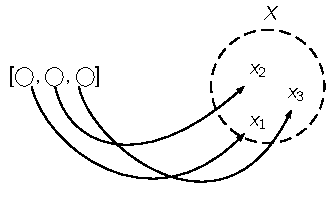
\includegraphics{img/container.pdf}
\end{center}
\caption{Llenando un container de lista}
\label{fig:List}
\end{figure}

Generalizando, llenar un container con valores de un tipo \AgdaBound{X}, es proveer una función que asigne valores de \AgdaBound{X} a cada posición, para cada forma. Llamaremos a esta función, la {\it extensión} del container.
 

\section{Definición y extensión}

A continuación expondremos formalmente esta nueva forma de representación. Para dar una instancia de un nuevo constructor de tipo proveeremos por un lado su estructura en la forma de un {\it container}. Luego, para permitir ``llenar'' al container con datos de tipo \AgdaBound{X}, calcularemos su {\it extensión}. 

%%%%%%%%%%%%%%%%%%%%%%%%%%%%%%%%%%%%%%%%%%%%%%%%
%%     DEFINICION    
%%%%%%%%%%%%%%%%%%%%%%%%%%%%%%%%%%%%%%%%%%%%%%%%

\subsection{Definición}

\begin{definition}
  Un {\it container} es un par ({\it Sh}, {\it Pos}) que notamos \agdaCont{Sh}{Pos} donde

  \begin{itemize}
  \item {\it Sh} es un conjunto de {\it formas} (o {\it shapes} en inglés).
  \item {\it Pos} es es un conjunto de posiciones, para cada forma $s$ en $Sh$. 
      Es decir, es una familia de posiciones indexada por las formas.
  \end{itemize}
\end{definition}


En Agda definimos: 

\begin{agdacode}\label{code:cont}{\it Containers}

\ExecuteMetaData[latex/Container.tex]{cont}
\end{agdacode}

Recordemos que en Agda un record es una tupla donde se le asigna nombre a cada componente y, opcionalmente, un constructor de instancias. Los nombres asignados a cada componente hacen a su vez las veces de destructores del record.
En el caso de \AgdaDatatype{Cont}, construimos sus instancias llamando a  \AgdaInductiveConstructor{$\_\tri\_$} con un \AgdaBound{S} : \AgdaDatatype{Set} y un \AgdaBound{P} : \AgdaBound{S} $\to$ \AgdaDatatype{Set}. Notar que el tipo de los componentes de un record puede depender de componentes anteriores.

Los nombres de campos \Sh y \Pos del record \AgdaDatatype{Cont} definen funciones de destrucción, con tipos:

\sangrar
\Sh : \AgdaDatatype{Cont} $\to$ \AgdaDatatype{Set}

\sangrar
\Pos : (C : \AgdaDatatype{Cont}) $\to$ \Sh C $\to$ \AgdaDatatype{Set}\\
de forma tal que para todo C : \AgdaDatatype{Cont} siempre valga la siguiente igualdad definicional: \Sh C \AgdaInductiveConstructor{$\tri$} \Pos C = C .

\begin{example}
Volviendo al ejemplo de la sección \ref{sec:containers.motivacion},
el container que representa a las listas está dado por el elemento \AgdaFunction{cList}, definido como:

 \ExecuteMetaData[latex/Examples.tex]{clist}

Aludiendo a lo expuesto anteriormente, las listas son aquél tipo cuya forma está dada por su longitud. Es decir, el conjunto de todas las formas posibles será el conjunto de los números naturales y el cero. Fijada una longitud \AgdaBound{n}, el conjunto de posiciones será el de todos los enteros entre \AgdaBound{0} y \AgdaBound{n - 1}. Es decir, es el \AgdaBound{n}-ésimo conjunto finitario.
\end{example}

%%%%%%%%%%%%%%%%%%%%%%%%%%%%%%%%%%%%%%%%%%%%%%%%
%%     EXTENSION    
%%%%%%%%%%%%%%%%%%%%%%%%%%%%%%%%%%%%%%%%%%%%%%%%
 
\subsection{Extensión}
  
Hasta ahora hemos expuesto la forma en que el universo sintáctico de
containers representa a ciertos constructores de tipos. Algunas preguntas que caben hacerse son: ¿Qué constructores son posibles de ser representados como containers? En otras palabras, ¿a qué constructores representan los containers? ¿Cómo estar seguros, más allá de la apelación a la intuición, que un container representa a un constructor determinado?

Antes de contestar esas, entre otras cuestiones, trataremos de dar respuesta a una pregunta más elemental y por lo tanto de más sutil respuesta: ¿Qué es un constructor de tipos?
Una idea intuitiva fue ofrecida al comenzar el capítulo: un constructor de tipos construye un tipo a partir de otro dado genéricamente, en forma de parámetro.
Para ejemplificar dicha aseveración, dimos el elemento \AgdaDatatype{List}, en la definición \ref{list}.
Si observamos dicha definición podemos apreciar que el constructor de tipos \AgdaDatatype{List} tiene el siguiente tipo: 

\sangrar
\AgdaDatatype{List} \AgdaSymbol{:} \AgdaDatatype{Set} \AgdaSymbol{$\to$} \AgdaDatatype{Set}

Otro constructor de tipos posible podría ser, por ejemplo, el que construye pares de elementos de dos tipos distintos:

 \ExecuteMetaData[latex/Aux.tex]{pair}
 
Un ejemplo más, es el de las funciones de un tipo arbitrario en sí mismo. Es decir, el tipo de datos \AgdaDatatype{Endo} $X$, expuesto en el siguiente código, engloba a todas las funciones con tipo $X \to X$. 
 
 \ExecuteMetaData[latex/Aux.tex]{endo}

 Tanto el constructor de tipos \AgdaDatatype{Pair}, como el constructor \AgdaDatatype{Endo} no serán posibles de ser representados como containers. Esto se debe a que restringimos el análisis a {\it ciertos} constructores de tipo.
Por simplicidad, el tipo de datos \AgdaDatatype{Pair} no será contemplado, puesto que nos limitamos a constructores de un sólo argumento. Sin embargo, toda la teoría de containers se extiende fácilmente a constructores de más argumentos. En tal caso sí incluiríamos al tipo de los pares. 
 Por otro lado, tampoco podremos representar al tipo \AgdaDatatype{Endo} puesto que nos conciernen aquellos constructores que cumplen ciertas propiedades y a los que llamaremos {\it funtores}.


\begin{definition} \label{def:funtor}
  Un constructor de tipos \AgdaDatatype{F} \AgdaSymbol{:} \AgdaDatatype{Set} \AgdaSymbol{$\to$} \AgdaDatatype{Set} es un {\it funtor}~\cite{plotkin+reynolds} si existe una función de mapeo

 \ExecuteMetaData[latex/Aux.tex]{map}\\
 tal que

 \sangrar
 $
 \left \{ \begin{array}{ll}
 \AgdaFunction{map}\ \AgdaFunction{id} = \AgdaFunction{id} &
 \\ \AgdaFunction{map}\ f \circ \AgdaFunction{map}\ g = \AgdaFunction{map}\ (f\ \AgdaFunction{$\circ$}\ g) & \quad \forall\ f :  Z \to B,\ g : A \to Z
 \end{array}
 \right. 
 $
 
Es decir, un funtor es un constructor \AgdaDatatype{F} que cumple con ciertas propiedades extra. Siempre que exista una función entre los tipos $A$ y $B$ habrá una función entre \AgdaDatatype{F} $A$ y \AgdaDatatype{F} $B$ de forma tal que las identidades y composiciones se preserven. 
 
\end{definition}

\vspace{1ex}

El constructor de pares \AgdaDatatype{Pair}
no será funtor sino hasta que fijemos el tipo de uno de los dos elementos del par. Por ejemplo, fijando el primer tipo al de los naturales se obtiene:

 \ExecuteMetaData[latex/Aux.tex]{pairNX}

En el caso de \AgdaDatatype{Endo} no es posible definir una función \AgdaFunction{map} que cumpla con los requisitos de la definición.
 
\vspace{1ex}

Retomando nuestra exposición, presentaremos a continuación
la noción de {\it extensión} de un container, que hará posible volver a interpretarlos como constructores de tipos en su forma funtorial.

Si \AgdaBound{cF} \AgdaSymbol{:} \AgdaDatatype{Cont} es un container, entonces su extensión, que notamos \agdaExt{\AgdaBound{cF}}, será un funtor:

\sangrar
\agdaExt{\AgdaBound{cF}} \AgdaSymbol{:} \AgdaDatatype{Set} \AgdaSymbol{$\to$} \AgdaDatatype{Set}

Intuitivamente, la extensión permitirá llenar un container con valores del tipo argumento.
En caso en que necesitemos precisión en la exposición, llamaremos {\it funtor container} a un funtor obtenido de calcular la extensión a un container. 

\vspace{2ex}

\begin{definition}
  La {\it extensión} del container \agdaCont{S}{P} sobre el conjunto \AgdaBound{X} es el conjunto de pares $(s, f)$ donde $s \in S$ y $f : Ps \to X$.
  Lo notamos \agdaExt{\agdaCont{S}{P}}.

Dado un caso particular de forma, tenemos un conjunto de posiciones. La extensión requiere de una función de posiciones en valores. 

\begin{agdacode}\label{code:cont:ext}{\it Extensión de containers}

\ExecuteMetaData[latex/Container.tex]{ext}
\end{agdacode}

Dicho de otra forma, \agdaExt{\agdaCont{S}{P}}
define familias de funciones $P s \to X$ de posiciones en valores por cada forma $s$ del conjunto $S$.
\end{definition}

\begin{example}
Entonces, para completar nuestro ejemplo de las listas, podemos finalmente calcular su extensión y así volver al <<mundo real>>. 

\ExecuteMetaData[latex/Examples.tex]{list}

Incluso es posible definir los constructores originales del tipo \AgdaDatatype{List} dado inductivamente:

\ExecuteMetaData[latex/Examples.tex]{listconstructors}

Dado que la forma de una lista es su longitud, el valor 
\AgdaFunction{nil} construye un elemento con forma igual a \AgdaNumber{0}. La función que asigna valores a posiciones es la función vacía, representada en Agda por $(\lambda\; ())$, ya que la forma nula no tiene posiciones.
Por su parte, la función \AgdaFunction{cons} \AgdaBound{x} construye una lista cuya forma es el sucesor de la lista argumento, puesto que \AgdaFunction{cons} aumenta su longitud en uno. Además, ahora la posición \AgdaInductiveConstructor{zero} mapea al nuevo elemento \AgdaBound{x}, desplazando al resto.
\end{example}

  A pesar de haber sostenido que los containers nos proveen una forma de construir funtores recurriendo al cálculo de su extensión, nos queda pendiente evidenciar que esto es cierto. Intuitivamente, si un container es un esqueleto donde se guardarán datos, resulta lógico que los datos almacenados puedan ser modificados sin tocar ese esqueleto que los contiene.
  A continuación definimos la función \AgdaFunction{map} de containers. Queda pendiente demostrar que dicha función cumple con los requerimientos de la definición \ref{def:funtor}

\begin{definition} Sea $f$ una función de $X$ en $Y$ y $C$ un container. Se define el mapeo de $f$ sobre el funtor container \agdaExt{$C$} como una nueva función de \agdaExt{$C$} $X$ en \agdaExt{$C$} $Y$ que preserva las formas y aplica $f$ a los elementos almacenados, como se indica a continuación:

\ExecuteMetaData[latex/Container.tex]{map}
\end{definition}

Así como vemos que la extensión de un container resulta ser un endofuntor en \AgdaDatatype{Set}, y que lógicamente dichos funtores pueden componerse y obtener así otro funtor, también podemos componer containers antes de calcular su extensión. Es decir, los containers son cerrados bajo composición, siendo la extensión de la composición equivalente a la composición de las extensiones.

\begin{definition} Definimos la composición de los containers $C$ y $D$ como el container que tiene por conjunto de formas posibles a \agdaExt{$C$} (\AgdaField{Sh} $D$). Es decir que por cada posición en una forma $c$ de $C$, tenemos una forma de $D$.

  Dada una forma $(c,d)$, siendo $c$ forma de $C$ y $d$ una función de posiciones en $C$ hacia formas en $D$, el conjunto de posiciones es el conjunto de pares dependientes $(p,q)$, donde $p$ es una posición en $C$ en la forma $c$ y $q$ una posición de $D$ en la forma $(d \, p)$.

  \ExecuteMetaData[latex/Composition.tex]{compose}
\end{definition}

Componer constructores de tipos da como resultado constructores en cierta forma {\it anidados}. Con la composición podemos formar, por ejemplo, las listas de árboles o los árboles de listas. En el siguiente código vemos la construcción del tipo \AgdaFunction{maybeSthg} $C$, que no es más que el constructor $C$ equipado de un valor extra. 

\begin{example} {\it Composición del constructor de tipos \AgdaDatatype{Maybe} con cualquier otro constructor $C$}
  
  \ExecuteMetaData[latex/Examples.tex]{maybeSthg}
\end{example}

\vspace{3ex}

En conclusión, hemos expuesto una sintaxis para representar ciertos constructores de tipo funtoriales \AgdaDatatype{F} \AgdaSymbol{:} \AgdaDatatype{Set} \AgdaSymbol{$\to$} \AgdaDatatype{Set} como un container
\AgdaFunction{cF} \AgdaSymbol{:} \AgdaDatatype{Cont}.
La función de extensión se constituye como un mecanismo para obtener nuevamente un funtor, tal que \agdaExt{\AgdaFunction{cF}} $\cong$
\AgdaDatatype{F}.

\subsection{Ejemplos}

%%%%%%%%%%%%%%%%%%%%%%%%%%%%%%%%%%%%%%%%%%%%%%%%
%%     ID
%%%%%%%%%%%%%%%%%%%%%%%%%%%%%%%%%%%%%%%%%%%%%%%%

\begin{example}
  Comencemos con uno de los ejemplos más sencillos que podamos construir: el container que define al tipo identidad.
  Recordemos la definición canónica de \AgdaDatatype{Id}, expresada en Agda:

  \ExecuteMetaData[latex/Aux.tex]{id}
  
  En este caso tenemos una única forma posible, con una única posición.

\begin{center}
\AgdaInductiveConstructor{identity}$\bigcirc$
\end{center}

  El elemento que simbolizará al tipo \AgdaDatatype{Id} en el universo de containers será el siguiente, siendo \AgdaDatatype{$\top$} el conjunto que tiene a \AgdaInductiveConstructor{tt} como único el elemento.

  \ExecuteMetaData[latex/Examples.tex]{cId}

  
  Al extender dicho container, obtenemos un constructor de tipos \AgdaDatatype{Id}. Podemos definir también el constructor de datos \AgdaFunction{identity}.

  \ExecuteMetaData[latex/Examples.tex]{Id}
\end{example}
\vspace{2ex}


%%%%%%%%%%%%%%%%%%%%%%%%%%%%%%%%%%%%%%%%%%%%%%%%
%%     K
%%%%%%%%%%%%%%%%%%%%%%%%%%%%%%%%%%%%%%%%%%%%%%%%

\begin{example} \label{cont:k}
  Otro ejemplo trivial es el del container que construye el funtor constante. Es decir, aquél que ignora totalmente el tipo argumento y retorna un tipo constante fijado previamente.

 \ExecuteMetaData[latex/Examples.tex]{cK}

 Las formas posibles serán exactamente los elementos del tipo constante, careciendo todas ellas de posiciones, puesto que pretendemos ignorar al tipo argumento. 
 El funtor container asociado resulta:

 \ExecuteMetaData[latex/Examples.tex]{K}

 Por ejemplo, el tipo \AgdaDatatype{K $\Nat\ \bot$} construye los naturales ignorando al tipo \AgdaDatatype{$\bot$}. Un habitante posible será:

 \ExecuteMetaData[latex/Examples.tex]{dos}

 %% No está de más resaltar que si no se ignorara al tipo argumento, entonces sería imposible de construir el valor \AgdaFunction{dos} o cualquier otra instancia, dado que \AgdaDatatype{$\bot$} es el tipo vacío.
  
\end{example}
\vspace{2ex}

%%%%%%%%%%%%%%%%%%%%%%%%%%%%%%%%%%%%%%%%%%%%%%%%
%%     MAYBE
%%%%%%%%%%%%%%%%%%%%%%%%%%%%%%%%%%%%%%%%%%%%%%%%

\begin{example} El constructor de datos \AgdaDatatype{Maybe} es aquél que agrega un elemento al tipo argumento.
Un valor de tipo \AgdaDatatype{Maybe} \AgdaBound{X} contiene o bien un valor \AgdaBound{x} de tipo \AgdaBound{X} (representado por el elemento \AgdaInductiveConstructor{just} \AgdaBound{x} ) o bien nada (representado por el valor \AgdaInductiveConstructor{nothing}). La utilización de \AgdaDatatype{Maybe} es una estrategia para lidiar con errores o casos excepcionales y resulta fundamental a la hora de escribir programas totales. 
  Se define inductivamente como:
  
  \ExecuteMetaData[latex/Aux.tex]{maybe}

  Queremos construir una porción de sintaxis que represente a los esqueletos de \AgdaDatatype{Maybe}, i.e., queremos construir un container. Las formas posibles que tendrán los datos son dos:

  \begin{center}
  \AgdaInductiveConstructor{nothing} $\quad$ \AgdaInductiveConstructor{just}$\bigcirc$
  \end{center}
  
  La primera forma carece de posiciones y la segunda tiene una única posición. Definimos entonces el container \AgdaDatatype{cMaybe} como:

  \ExecuteMetaData[latex/Examples.tex]{cMaybe}

  Al igual que hicimos con el tipo \AgdaDatatype{Id}, calculamos su extensión y definimos los constructores de datos.

\ExecuteMetaData[latex/Examples.tex]{maybe}
\end{example}
\vspace{2ex}


%%%%%%%%%%%%%%%%%%%%%%%%%%%%%%%%%%%%%%%%%%%%%%%%
%%     STREAM
%%%%%%%%%%%%%%%%%%%%%%%%%%%%%%%%%%%%%%%%%%%%%%%%

\begin{example} \label{example:stream}Un ejemplo muy interesante de analizar es el del tipo \AgdaDatatype{Stream}. Un stream es una secuencia infinita numerable de valores. Una posible definición de este tipo de datos es:

\ExecuteMetaData[latex/Aux.tex]{stream}

Resulta importante evidenciar que es imposible construir un elemento de este tipo en Agda, dado que el chequeo de terminación nos lo impide. Por ejemplo, si quisiéramos construir una secuencia infinita trivial de unos:

\sangrar
\AgdaTerminationProblem{\AgdaFunction{s}} : \AgdaDatatype{Stream} \AgdaDatatype{$\Nat$}

\hspace{2.5ex}
\AgdaFunction{s} = \AgdaNumber{1} \AgdaInductiveConstructor{$::$} \AgdaTerminationProblem{\AgdaFunction{s}}

El recuadro naranja es la simbología que usa Agda para indicar que no puede construir una función debido a que no puede garantizar su terminación. 
Por lo tanto, dicho tipo de datos se define de forma coinductiva:

\ExecuteMetaData[latex/Stream.tex]{stream}

Ahora sí podemos definir el stream de unos:

\ExecuteMetaData[latex/Stream.tex]{stream1s}

Para pensar en una representación con containers de los streams, tenemos que dar, por un lado, un conjunto de formas. A diferencia de las listas, que podían ser de longitudes arbitrariamente grandes pero siempre finitas, los streams tienen todos una única longitud, y por lo tanto una única forma. Las posiciones en esa única forma son tantas como naturales haya. Se define entonces el container que representa al constructor de streams como:

\ExecuteMetaData[latex/Examples.tex]{cStream}

El container funtor \AgdaDatatype{Stream} y la secuencia infinita de unos que llamamos \AgdaFunction{s}, están dados por:

\ExecuteMetaData[latex/Examples.tex]{Stream}

Advertir una ventaja que nos proveen los containers: no necesitamos apelar a toda la construcción coinductiva, de la misma forma que evitamos el uso de la inducción en los ejemplos previos. %Sin embargo, hay casos donde estos mecanismos pueden resultar de gran valor. 

\end{example}

%%%%%%%%%%%%%%%%%%%%%%%%%%%%%%%%%%%%%%%%%%%%%%%%
%%     READER
%%%%%%%%%%%%%%%%%%%%%%%%%%%%%%%%%%%%%%%%%%%%%%%%

\begin{example}
  Para representar computaciones que dependen de valores en un entorno compartido e inmutable, la programación funcional modela la dependencia como una función. El tipo de datos \AgdaDatatype{Reader} \AgdaBound{E} encapsula este tipo de valores. Notar que no contamos con valores de tipo \AgdaBound{X}. No hasta que se provea un entorno \AgdaBound{E}.

  \ExecuteMetaData[latex/Aux.tex]{reader}

  Asumiendo que ya contamos con un elemento \AgdaBound{E}, las formas posibles para los datos se limita a una sola. Las posiciones sí son más. ¿Cuántas?. Pues si estamos modelando funciones de \AgdaBound{E}\AgdaSymbol{$\to$}\AgdaBound{X}, necesitamos guardar tantos \AgdaBound{X} como elementos haya en \AgdaBound{E}.
  
  \ExecuteMetaData[latex/Examples.tex]{cReader}

Finalmente, podemos construir toda la infraestructura auxiliar, una vez que hayamos vuelto al <<mundo real>>. 

\ExecuteMetaData[latex/Examples.tex]{reader} 

Observemos que el container \AgdaFunction{cReader} resulta ser una generalización del container \AgdaFunction{cStream} presentado en el ejemplo \ref{example:stream}, siendo este último equivalente a \AgdaFunction{cReader} \AgdaDatatype{$\Nat$}.

\end{example}
\vspace{2ex}

%% %%%%%%%%%%%%%%%%%%%%%%%%%%%%%%%%%%%%%%%%%%%%%%%%
%% %%     STATE    
%% %%%%%%%%%%%%%%%%%%%%%%%%%%%%%%%%%%%%%%%%%%%%%%%%

%% \begin{example}

%%   El tipo de datos \AgdaDatatype{State} describe funciones que consumen un estado y producen un resultado, junto con el estado modificado. Es una situación similar a la de \AgdaDatatype{Reader}, pero agregando la posibilidad de modificar ese entorno antes inmutable. Encapsulamos esta sitación definiendo:
  

%%   \ExecuteMetaData[latex/Aux.tex]{state}

%% Podemos pensar a este tipo de funciones modificadoras de estado de forma diseccionada. Modelando por un lado el cambio de estado, y por otro la obtención del valor de tipo \AgdaDatatype{X}.

%%   \ExecuteMetaData[latex/Aux2.tex]{state2}

%%   Fijado el tipo del estado, las formas posibles serán todas aquellas funciones de cambio de estado. Y de la misma forma que razonamos con \AgdaDatatype{cReader}, habrá tantas posiciones como elementos en el estado, para así obtener una función de estados en posiciones.

%% \ExecuteMetaData[latex/Examples.tex]{cState}

%% Una vez logrado construir la representación con containers, calcular su extensión y definir funciones auxiliares puede resultar ilustrativo:

%%   \ExecuteMetaData[latex/Examples.tex]{state}
%% \end{example}


%%%%%%%%%%%%%%%%%%%%%%%%%%%%%%%%%%%%%%%%%%%%%%%%
%%     ÁRBOLES
%%%%%%%%%%%%%%%%%%%%%%%%%%%%%%%%%%%%%%%%%%%%%%%%

\begin{example} \label{code:tree} Veamos cómo el constructor de los árboles binarios con la información en las hojas puede ser representado como container. El tipo de datos dado inductivamente es:
  
\ExecuteMetaData[latex/Aux.tex]{tree}

Un container de árbol será simplemente un árbol donde borramos la información que se almacena.
En la figura \ref{fig:Tree} se pueden apreciar algunas esqueletos posibles de árboles. 

\begin{figure}[H]
\begin{center}
  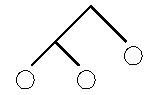
\includegraphics{img/tree1.pdf}\qquad\qquad
  \reflectbox{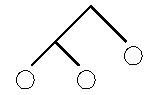
\includegraphics{img/tree1.pdf}}\quad\qquad
  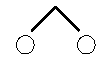
\includegraphics{img/tree2.pdf}
\end{center}
\caption{Containers de árbol}
\label{fig:Tree}
\end{figure}

La definición del conjunto de formas no difiere en mucho de la definición
inductiva del tipo \AgdaDatatype{Tree}.\footnote{Notar
  que lo mismo sucede con las listas. El conjunto de formas resulta
  ser el de los naturales, cuya definición tiene la misma estructura
  que la de las listas, sólo que ignorando los datos que se almacenan} 

\ExecuteMetaData[latex/Examples.tex]{treeSh}

Las posiciones posibles dependerán de las formas y serán tantas como
hojas haya. Por cada hoja hay una posición y para una forma \AgdaInductiveConstructor{nodeSh} $l\ r$, hay posiciones a la izquierda y a la derecha. 

\ExecuteMetaData[latex/Examples.tex]{treePos}

Finalmente, el container de los árboles binarios con datos en las hojas queda dado por:

\ExecuteMetaData[latex/Examples.tex]{ctree}


Observar que si quisiéramos representar árboles con la información almacenada en
los nodos, sólo cambiaríamos el conjunto de las posiciones, que dependerá de cuántos nodos tenga cada forma.

Otra cuestión interesante de destacar es el nivel de complejidad de notación que se alcanza al momento de representar árboles. En el capítulo \ref{chapter:construcciones} veremos que contamos con ciertos mecanismos de construcción de containers que proveen una suerte de modularidad, pudiendo componer containers de diversas maneras.
Estudiaremos allí un álgebra de containers.
\end{example}


\section{Morfismos de containers}

En esta sección presentaremos una forma de escribir funciones polimórficas entre tipos funtoriales. La estrategia a seguir es similar a la tomada en la sección anterior. Proveeremos una forma de definir conjuntos de códigos sintácticos, que habremos de llamar {\it morfismos de containers} y una función de extensión que los reinterprete.

Sean los containers
\AgdaFunction{cF}, \AgdaFunction{cG} \AgdaSymbol{:} \AgdaDatatype{Cont}
que representan a los constructores de tipos \AgdaDatatype{F}, \AgdaDatatype{G}  \AgdaSymbol{:} \AgdaDatatype{Set} \AgdaSymbol{$\to$} \AgdaDatatype{Set} respectivamente.
Es decir, \agdaExt{\AgdaFunction{cF}} $\cong$ \AgdaDatatype{F} y \agdaExt{\AgdaFunction{cG}} $\cong$ \AgdaDatatype{G}.

El objetivo es presentar una forma de representar ciertas funciones
\AgdaFunction{f} : \AgdaSymbol{$\forall$}\AgdaBound{$\{$X$\}\to$} \AgdaDatatype{F} \AgdaBound{X} \AgdaSymbol{$\to$} \AgdaDatatype{G} \AgdaBound{X}
como un morfismo de containers
\AgdaFunction{cf} : \AgdaFunction{cF} \AgdaFunction{$\Rightarrow$} \AgdaFunction{cG}.
En particular, nos interesan las \AgdaFunction{f} que 
preserven la estructura funtorial, es decir, que resulten ser {\it transformaciones naturales}.

\begin{definition} Sean los funtores \AgdaDatatype{F}, \AgdaDatatype{G}  \AgdaSymbol{:} \AgdaDatatype{Set} \AgdaSymbol{$\to$} \AgdaDatatype{Set}. Una función $f$ : \AgdaSymbol{$\forall$}\AgdaBound{$\{$X$\}\to$} \AgdaDatatype{F} \AgdaBound{X} \AgdaSymbol{$\to$} \AgdaDatatype{G} \AgdaBound{X} es una {\it transformación natural} si cumple, para toda $h : X \to Y$ y para alguna noción de igualdad.

\sangrar
\AgdaFunction{map} $h\ \circ$ $f$ = \AgdaFunction{f} $\circ$ \AgdaFunction{map} $h$

Notar que de cada lado de la igualdad, $f$ y \AgdaFunction{map} se instancian de forma diferente. Es decir, si agregamos los elementos implícitos como subíndices la ecuación de arriba nos queda: 

\sangrar
\AgdaFunction{map}$_{G}\ h\ \circ\ f_{X}$ = $f_{Y}\ \circ$ \AgdaFunction{map}$_{F}\ h$
\end{definition}

Para ello, definiremos un mecanismo de extensión que notaremos \agdaExtMorph{$\_$}\\ tal que
\agdaExtMorph{\AgdaFunction{cf}} : \AgdaSymbol{$\forall$}\AgdaBound{$\{$X$\}\to$} \agdaExt{\AgdaFunction{cF}} \AgdaBound{X} \AgdaSymbol{$\to$} \agdaExt{\AgdaFunction{cG}} \AgdaBound{X}
y así obtener
\agdaExtMorph{\AgdaFunction{cf}} $\cong$ \AgdaFunction{f}. La función \agdaExtMorph{\AgdaFunction{cf}} obtenida de extender el morfismo \AgdaFunction{cf} será una transformación natural entre los funtores container \agdaExt{\AgdaFunction{cF}} y \agdaExt{\AgdaFunction{cG}}.

\vspace{2ex}

Para comenzar la exposición analizaremos un ejemplo.
\begin{example}\label{ex:head}
Echemos un vistazo a la siguiente función, que retorna el primer elemento de una lista, si lo hay.

\ExecuteMetaData[latex/Aux.tex]{head}

Intuitivamente, un morfismo entre dos containers proveerá una forma de {\it reubicar} los elementos del primer container dentro del segundo.
¿Qué necesitamos proveer para crear una función \AgdaFunction{chead} que transforme un elemento de \AgdaFunction{cList} en uno de \AgdaFunction{cMaybe} de la forma esperada?
Por una lado necesitamos una función de \Sh \AgdaFunction{cList} en \Sh \AgdaFunction{cMaybe} para poder indicar que la lista vacía se transforma en el elemento \AgdaInductiveConstructor{nothing} y que para cualquier otra longitud de lista obtendremos la forma \AgdaInductiveConstructor{just} $\bigcirc$.  
Además necesitamos saber desde qué posiciones del container \AgdaFunction{cList} provienen los datos a guardar en el container imagen y así {\it reubicar} los valores almacenados. Para ello basta con dar una función que dada una posición de \AgdaFunction{cMaybe} nos indique una posición de \AgdaFunction{cList}, para cada forma.
En el caso de \AgdaFunction{head} habrá que indicar que el dato a guardar en la única posición de la forma \AgdaInductiveConstructor{just} $\bigcirc$ proviene de la primera posición de una lista de al menos un elemento, como muestra la figura \ref{fig:morph}.

\begin{figure}[H]
\begin{center}
  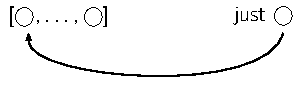
\includegraphics{img/morfismo2.pdf}
\end{center}
\caption{reubicando las posiciones según el comportamiento de \AgdaFunction{head}}
\label{fig:morph}
\end{figure}
\end{example}


\subsection{Definición y extensión de morfismos de container}

\begin{definition}
  Un {\it morfismo de containers} entre los containers $C_1$ y $C_2$ es un par de funciones $(m_{Sh}, m_{Pos})$, donde
  \begin{itemize}
    \item $m_{Sh}$ es una función que mapea las formas de $C_1$ hacia las formas de $C_2$
    \item Por cada forma $s$ de $C_1$, $m_{Pos}$ es una función que mapea cada posición de $C_2$ en la forma $m_{Sh}\ s$ hacia las posiciones de $C_1$ en la forma $s$.
  \end{itemize}
\end{definition}

Su formalización en Agda se expresa en el siguiente código:
\begin{agdacode}\label{code:morph}{\it Formalización de los morfismos de containers}

\ExecuteMetaData[latex/Container.tex]{morph}
\end{agdacode}

La componente \mSh del morfismo indica cómo transformar cada elemento del primer conjunto de formas en uno del segundo. La función \mPos es la encargada de reubicar los elementos a almacenar, indicando para cada posición del container imagen, una posición en el container origen.

\begin{definition} Sea $f$ un morfismo entre los containers $C$ y $D$. La {\it extensión} de $f$ sobre un conjunto $X$, que notamos \agdaExtMorph{$f$}, es una función entre los funtores containers \agdaExt{$C$} y \agdaExt{$D$} dada por el siguiente código:

\begin{agdacode}\label{code:morph:ext}{\it Extensión de morfismos de containers}

\ExecuteMetaData[latex/Container.tex]{morphExt}
\end{agdacode}

Al aplicar \agdaExtMorph{$f$} al elemento dado por una forma $c_s$ y una función $c_p$ de posiciones en valores, obtenemos otro container. Su forma la obtenemos gracias a la aplicación de la función de formas \mSh $f$. Dada una posición en esta nueva forma, \mPos $f$ indicará de dónde provienen los datos a guardar allí, información que completará la función $c_p$ .
\end{definition}

Un resultado muy interesante de esta construcción es que los morfismos de containers representan exactamente al conjunto de las transformaciones naturales entre los funtores \agdaExt{$C$} y \agdaExt{$D$}. Utilizando el universo de containers y morfismos nos aseguramos que las funciones definidas entre dos funtores containers serán transformaciones naturales, siendo imposible definir algo que no lo sea. Más aún, toda transformación natural $t$ entre \agdaExt{$C$} y \agdaExt{$D$} es representable en el universo de morfismos de containers por un elemento $f$, de forma tal que $\agdaExtMorph{$f$} = t$.

\begin{example} Para completar el ejemplo \ref{ex:head} expuesto en la introducción, veamos finalmente cómo queda definido el morfismo \AgdaFunction{chead}:

\ExecuteMetaData[latex/Examples.tex]{chead}

La función entre formas mapea la longitud de lista cero al elemento \AgdaInductiveConstructor{false}, representante del constructor \AgdaInductiveConstructor{nothing}. Para cualquier otra longitud de lista la forma resultante es \AgdaInductiveConstructor{true}, que indicaba la forma \AgdaInductiveConstructor{just}.

La función entre posiciones es vacía para el caso de las listas vacías puesto que allí no existen posiciones. En cualquier otra situación se mapea la posición única \AgdaInductiveConstructor{tt} a la primera de la lista. 

\ExecuteMetaData[latex/Examples.tex]{head}
\end{example}

\begin{definition}\label{code:morph:comp}Se define la {\it composición} entre dos morfismos de containers componiendo respectivamente las funciones de formas y posiciones, según se muestra en el siguiente código:
  
\ExecuteMetaData[latex/Container.tex]{morphComp}
\end{definition}

\begin{example}\label{code:morph:id}{\it Morfismos de containers identidad}

Dado cualquier container $C$, existe el morfismo identidad, que deja fija las formas y las posiciones.
  
  \ExecuteMetaData[latex/Container.tex]{morphId}
  Notar que la extensión de dicho morfismo será la función identidad.
\end{example}

\subsection{Equivalencia de morfismos}

Un lema que nos resultará muy útil para demostrar equivalencias en esta sección es aquél que prueba la igualdad de morfismos de containers. Dos morfismos de containers $f$ y $g$ son equivalentes siempre que lo sean sus componentes, las funciones de formas y posiciones.

\begin{agdacode}\label{morph:equivalence}{\it Equivalencia entre morfismos de containers}
  
\ExecuteMetaData[latex/Container.tex]{equivalence}
\end{agdacode}

Este es un claro ejemplo donde Agda no puede resolver trivialmente una equivalencia por no poder unificar los tipos de los argumentos.
Agda sólo nos permite probar por \AgdaInductiveConstructor{refl} una vez hecho pattern matching en los argumentos de \AgdaFunction{mEq}.
Esto es así puesto que sólo una vez probada la equivalencia de las funciones de formas, las funciones de posiciones tienen exactamente el mismo tipo.

Entonces, yendo paso a paso, el único habitante de \mSh $f$ \AgdaFunction{$\cong$} \mSh $g$ es \AgdaInductiveConstructor{refl}. Indicado esto, Agda unifica esta equivalencia y es posible hacer pattern matching en el segundo argumento. Al unificar la prueba de \mPos $f$ \AgdaFunction{$\cong$} \mPos $g$ la prueba final resulta trivial. 


\section{Categoría de containers}\label{cont:cat}

Dedicamos esta sección a presentar la formalización de los containers como una categoría. Los objetos de la categoría, que habremos de llamar $\Cont$ resultan ser los containers, definidos en \ref{code:cont}. El conjunto de morfismos será el de los morfismos de containers, expuesto en \ref{code:morph}. Como hemos mostrado en \ref{code:morph:comp} y \ref{code:morph:id}, los morfismos pueden componerse y siempre existe la identidad.

\begin{agdacode}\label{code:cont:cat}{\it Categoría de containers}

\ExecuteMetaData[latex/CatCont.tex]{cont}
\end{agdacode}

\chapter{Construcciones con containers}\label{chapter:construcciones}

\begin{epigraphs}
\qitem{
Se conservaron algunos adjetivos de hoy en día como bueno, fuerte, grande, negro, blando, pero en un número muy reducido. Por otra parte, su necesidad era mínima, ya que se llegaba a cualquier significado adjetival añadiendo {\it lleno} a un sustantivo-verbo. (...) Además, a cualquier palabra —y esto, como principio, se aplicaba a todas las palabras del idioma—, se le daba sentido de negación añadiendo el prefijo {\it in} o se le daba fuerza con el sufijo {\it plus}, o para aumentar el énfasis, {\it dobleplus}.}{1984\\ George Orwell}
\end{epigraphs}

En este capítulo presentaremos una serie de construcciones
que no solo aportarán a la modularidad de uso del universo de containers, apuntando a la programación genérica, sino que también clasificarán a la categoría de containers dentro de ciertas colecciones de categorías con propiedades interesantes, las categorías cartesianas cerradas.

Hemos visto en el capítulo \ref{cont} que los containers resultan ser una codificación válida de ciertos constructores de tipos. Desde este punto de vista propondremos formas genéricas de construir, por ejemplo, a partir de un par de constructores, el constructor de pares.
Pensando lo antedicho en términos algebraicos, podemos intuir que hablamos de un operador producto sobre containers y su clausura. Es decir, que los containers son cerrados bajo alguna definición de producto. Si bien en términos particulares eso es cierto, nos interesa asimismo tomar un punto de vista aún más general, retomando las nociones de teoría de categorías expuestas en las preliminares y continuadas en el capítulo \ref{cont}. De esta forma, veremos lo que significa que una categoría {\it cuente con productos}. Hecho esto, mostraremos que la categoría $\Cont$ de containers y sus morfismos, efectivamente cuenta con ellos.
Además del producto, presentaremos las construcciones de coproducto, exponencial, objetos inicial y terminal y veremos brevemente porqué se las denomina {\it construcciones universales}.

Debido a que no asumimos conocimientos previos de teoría de categorías, para cada construcción abstracta comenzaremos introduciendo brevemente su dimensión categórica. Para ello, se impulsará al lector a pensar desde lo particular --la teoría de conjuntos-- hacia lo general --la teoría de categorías-- y así motivar la introducción de cada nuevo concepto categórico a partir de la abstracción de un caso particular, siguiendo un camino similar al transitado por algunos libros de referencia~\cite{Awodey,BarrWells}.   
Con esta base expondremos una formalización genérica en código Agda, extendiendo lo presentado en la sección \ref{cat}. 
Finalmente, exhibiremos la forma que tienen dichas construcciones sobre containers. Cuando sea posible daremos también una interpretación menos abstracta, en teoría de la programación, siguiendo la línea de presentación del capítulo \ref{cont}, con ejemplos y análisis particulares al caso.


\section{Coproducto}\label{cons:coprod}

\subsection{Motivación: (De)construyendo el coproducto}

Muchas de las construcciones de teoría de categorías pueden pensarse a partir de la teoría de conjuntos, con vistas a la generalización. En efecto, muchas de estas nociones categóricas han surgido de esta manera. 
Nuestra meta en esta sección de motivación es tratar de seguir ese proceso que va desde lo particular a lo general para así comprender más profundamente la construcción de {\it coproducto} que nos concierne analizar en esta parte del trabajo.

La unión disjunta de conjuntos, que notamos $\uplus$, es la modificación de la unión clásica de conjuntos donde se {\it etiquetan} los elementos según el conjunto desde el que provienen. Para mayor claridad, observemos el siguiente ejemplo, donde las {\it etiquetas} se muestran como subíndices:
\begin{center}
\begin{tabular}{c c c c}
  $A$ & $B$ & $A \cup B$ & $A \uplus B$ \\
  $\{ x , y \}$ & $\{ x, z, w \}$ &  $\{ x, y, z , w \}$ & $\{ x_{A} , y_{A}, x_{B}, z_{B}, w_{B} \}$
\end{tabular}
\end{center}


Notar que con esta modificación la operación deja de ser idempotente: unir disjuntamente un conjunto consigo mismo traerá como resultado la duplicación de sus elementos.

Un habitante de la unión disjunta de dos conjuntos será o bien un elemento del primer conjunto o bien uno del segundo. En el caso de los conjuntos, el coproducto nos permite codificar una opción, una disyunción.
En programación suele utilizarse esta construcción para expresar que un elemento es {\it o bien} de tipo $A$ {\it o bien} de tipo $B$.
 En Agda suele definirse como:

\begin{agdacode}{\it Unión disjunta de conjuntos}\label{code:uplus}
  
\ExecuteMetaData[latex/Aux.tex]{uplus}
\end{agdacode}

En resumidas cuentas, un elemento del conjunto $A$ \AgdaFunction{$\uplus$} $B$ es {\it o bien} un valor de la forma \AgdaInductiveConstructor{inj$_1$} $a$ (con $a\, :\, A$) {\it o bien} un valor de la forma \AgdaInductiveConstructor{inj$_2$} $b$ (con $b\, :\, B$). 
A las funciones de etiquetado suele designárseles los nombres de {\it inyecciones}, el nombre \AgdaInductiveConstructor{inj} proviene del vocablo inglés {\it injection}. Se las denomina de esa manera porque se considera que inyectan en el objeto coproducto la información de los sumandos.

Volviendo a teoría de categorías, hemos mencionado en la sección \ref{cat} que dicha teoría hace hincapié en las relaciones entre los objetos más que en los objetos en sí mismos. Dicho de otra forma, son los morfismos los que capturan la esencia de cada idea. Trataremos entonces de expresar cada concepto que nos interesa de la teoría de conjuntos centrándonos en las funciones que acompañan a cada construcción, es decir, en las relaciones entre los conjuntos involucrados.
Sin embargo, la definición recientemente expuesta hace justamente lo que queremos evitar: referirse a los habitantes de los conjuntos. Para comenzar a independizarnos de ellos podemos preguntarnos cómo definir un objeto coproducto a partir de las relaciones que podemos percibir entre los objetos.

En términos particulares, dados dos conjuntos $A$ y $B$, ¿qué relación tienen con su unión disjunta? ¿qué función involucra a $A$ y a $B$ con $A \uplus B$? 
Por empezar, siempre podremos construir funciones que vayan desde cada conjunto hacia su unión disjunta, las funciones de inyección.  
Con esto en mente, podríamos pensar entonces al coproducto como un objeto equipado con dos morfismos desde cada objeto factor hacia él.

Pero no cualquier objeto de estas características es el objeto coproducto, ya que claramente no cualquier conjunto $C$ y par de funciones que vayan de $A$ y $B$ hacia $C$ resulta ser la unión disjunta. Entonces, para indicar porqué otro objeto {\it no} es el coproducto, habrá que involucrar también a las relaciones entre el verdadero objeto coproducto que estamos definiendo y {\it cualquier otro} objeto de la categoría que se postule como tal. Siendo $C$ un conjunto cualquiera y $f: A \to C,\ g: B \to C $ funciones, ¿qué hace que $C$ no sea un buen candidato a ser el objeto coproducto? ¿qué relación encontramos entre $C$ y $A\uplus B$? Pues desde la unión disjunta {\it siempre} podremos construir una función hacia  este objeto $C$ simplemente eligiendo qué función aplicar, si $f$ o $g$. Aún más, dicha función es la única entre $A\uplus B$ y $C$ con estas características. La definimos como:


\begin{agdacode}\hspace{3ex}\label{code:choice}
  
\ExecuteMetaData[latex/Aux.tex]{choice}
\end{agdacode}

Luego de haber desmenuzado a la unión disjunta de conjuntos en aras de la generalidad categórica, continuaremos la exposición con la definición formal de coproductos en una categoría.

\subsection{Definición y formalización}
\begin{definition}\label{cat:coprod}
  Sean $A,B$ objetos de una categoría \C.
El {\it coproducto} de $A$ y $B$ es un objeto $A + B$, junto con dos morfismos
\flecha{A}{\iota_1}{A + B} y
\flecha{B}{\iota_2}{A + B} 
tal que para todo otro objeto $C$ y par de morfismos $\flecha{A}{f}{C},\ \flecha{B}{g}{C}$ de la categoría, exista un único morfismo $[ f,g ]$ que haga conmutar al siguiente diagrama
:
\begin{center}
  \xymatrixcolsep{3pc} \xymatrixrowsep{3pc}
  \centerline{\xymatrix{ 
      & C   & \\
      A \ar[ur]^{f} \ar[r]_{\iota_1} & A + B \ar@{-->}[u]_{[f,g]} & B \ar[l]^{\iota_2} \ar[ul]_{g}}}
\end{center}
\end{definition}

Los morfismos como $[f,g]$ suelen denominarse {\it mediales} por ser los que atraviesan el diagrama conmutativo. En el caso particular del coproducto, lo llamaremos morfismo de {\it coreunión}. La representación del morfismo como una flecha con línea de puntos en el diagrama conmutativo es un recurso para expresar unicidad. Es decir, para que el objeto $A + B$ cumpla con la definición, debe existir un único morfismo $\flecha{A+B}{}{C}$ que haga conmutar al diagrama.

Cuando para cada par de objetos de una categoría existe su objeto coproducto, decimos que la categoría {\it cuenta con coproductos}.

Habiendo definido al objeto coproducto podemos mencionar de qué se tratan las {\it construcciones universales}, al menos sin referirnos a los pormenores del asunto. En general, cuando hablamos del ``mejor objeto'' que cumpla con ciertas propiedades, como lo hicimos con el coproducto, nos estamos refiriendo a una construcción universal. Muchas veces con ``mejor'' nos referimos a menor, mayor, con menos restricciones, etc.

Las propiedades universales son ubicuas en la matemática. La teoría de categorías apunta a analizarlas desde un punto de vista abstracto y así comprenderlas en su totalidad, evitando repetir el estudio de cada instancia en particular. Por ejemplo, sabemos que las propiedades universales definen objetos que resultan ser únicos, salvo isomorfismos únicos. Particularmente, puede demostrarse que todo objeto coproducto de otros dos es único hasta isomorfismos. Esto significa que es posible que exista más de un objeto coproducto dados otros dos, pero todos ellos serán isomorfos. 

\vspace{3ex}

Como nota de color resulta interesante mencionar que otra denominación para los coproductos que suele encontrarse en la bibliografía es la de {\it suma}, siendo un nombre más intuitivo, sobre todo cuando pensamos en ciertas categorías. El apelativo {\it coproducto} se origina en el hábito de denominar co-{\it concepto} al dual de un {\it concepto}. Recordemos que la categoría dual $\C^{op}$ de una categoría $\C$ es aquella que se obtiene al revertir el sentido de los morfismos. De este modo, un co-{\it concepto} en una categoría $\C$ es un {\it concepto} en $\C^{op}$. Veremos en la sección \ref{cons:prod} que la idea de {\it producto} puede pensarse en los mismos términos que el coproducto, pero revirtiendo el sentido de las flechas del diagrama conmutativo. Dicho esto cabe preguntarse: ¿porqué entonces no se llama {\it cosuma} al producto? Pues porque en teoría de categorías, el producto fue concebido primero. En 1950, Saunders Mac Lane~\cite{maclane1950} presenta lo que sería muy probablemente el ejemplo más remoto de uso de la teoría de categorías para definir una noción matemática fundamental\footnote{Ver~\cite{Awodey}}. 

\vspace{3ex}

A continuación formalizaremos en Agda lo presentado hasta aquí. Seguiremos los pasos de la sección \ref{cat} y extenderemos dicho modelo para permitir expresar cuándo una categoría tiene coproductos.

Como expusimos anteriormente, Agda nos permite definir estructuras algebraicas que incluyan no sólo al portador con sus operaciones sino también las propiedades que se deben cumplir.
El código \ref{code:hasCoproducts} formaliza lo presentado, definiendo una estructura de record indexado por una categoría \AgdaBound{\C}. Dar una instancia de \AgdaFunction{HasCoproducts} \AgdaBound{\C} implica probar que la categoría \AgdaBound{\C} cuenta con coproductos.

\begin{agdacode}{\it Formalización de categoría con coproductos}\hspace{3ex}\label{code:hasCoproducts}
  
\ExecuteMetaData[latex/Cat.tex]{hasCoproducts}
\end{agdacode}

El elemento \AgdaField{Coprod} es el que construye cada objeto coproducto, dados otros dos. Los elementos \AgdaField{inl} e \AgdaField{inr} son morfismos en la categoría \AgdaBound{\C}, definidos para todo par de objetos \AgdaBound{X, Y} como las respectivas inyecciones. De forma similar se expresa la signatura del morfismo medial \AgdaField{copair}. 
Los campos dedicados a las pruebas garantizarán que las construcciones proporcionadas son las correctas, dado que hacen conmutar al diagrama de la definición \ref{cat:coprod}.



 Veamos a continuación cómo se manifiesta esta construcción en la categoría de containers.

\subsection{Coproducto de Containers}

Para formalizar el coproducto en la categoría de containers necesitamos contar con un elemento \AgdaField{Coprod} que arme un container a partir de otros dos. Será obligatorio definir también funciones \AgdaField{inl}, \AgdaField{inr} y \AgdaField{copair} que proyecten cada uno de los containers involucrados en un coproducto. Finalmente, habrá que suministrar las pruebas requeridas y así garantizar que estamos presentando la construcción correcta.  
En resumen, buscamos construir un elemento \AgdaFunction{ContHasCoproducts}, llenando los huecos del código \ref{cont:coprod:huecos} indicados con signos de interrogación y así formalizar la noción de que la categoría \AgdaFunction{$\Cont$} presentada en la sección \ref{cont:cat} tiene coproductos.
\begin{agdacode}\hspace{1ex}\label{cont:coprod:huecos}
  
\ExecuteMetaData[tex/AuxCatCont.tex]{hasCoproducts}
\end{agdacode}

A continuación se muestra el código del constructor \AgdaFunction{Either} que arma un coproducto a partir de dos containers $C$ y $D$. Por un lado, las formas de un container coproducto serán o bien formas de $C$ o bien formas de $D$. Por otro lado, hecha esa elección y determinada una forma $s$, las posiciones posibles dentro de ella dependerán del conjunto del que $s$ proviene. Si $s$ es una forma de $C$, entonces las posiciones posibles serán las posiciones de $C$ en $s$ y de forma similar en el caso en que $s$ sea forma de $D$.

\ExecuteMetaData[latex/Sum.tex]{either}

Renombramos como \AgdaFunction{$[\_,\_]_{\Set}$} al operador \AgdaFunction{[\_,\_]} presentado en el código \ref{code:choice} para dejar en claro que se trata del correspondiente a la categoría $\Set$ y no al que presentaremos próximamente, perteneciente a la categoría $\Cont$.

Lógicamente, las inyecciones serán morfismos en la categoría de containers. La primera componente del morfismo es la función sobre formas, que simplemente inyecta una forma de $C$ en el conjunto \Sh $C$ $\uplus$ \Sh $D$. Dada una forma $c$ de $C$, las posiciones en \AgdaFunction{Either} $C$ $D$ se reducen a posiciones de $C$ en $c$. La función de formas será simplemente la función identidad.

\ExecuteMetaData[latex/Sum.tex]{inj1}

La segunda inyección es análoga.

El morfismo de coreunión construye un morfismo a partir de otros dos, eligiendo aplicar uno u otro dependiendo del caso. La función de formas elegirá cuál de las respectivas funciones de formas aplicar. La nueva función de posiciones hará lo mismo con las respectivas funciones de posiciones originales. 

\ExecuteMetaData[latex/Sum.tex]{coreunion}

Para terminar, se requiere dar pruebas de haber construido el coproducto correctamente. Probaremos por un lado que
inyectar elementos al lado izquierdo de un coproducto para luego aplicar la coreunión es igual a sólo hacer lo que decide la coreunión sobre la parte izquierda. Igualmente sobre la parte derecha.
Es decir, queremos construir elementos de \AgdaFunction{$[$} $f , g$ \AgdaFunction{$]\ \circ\ \iota_{1} \cong$} $f$ y de \AgdaFunction{$[$} $f , g$ \AgdaFunction{$]\ \circ\ \iota_{2} \cong$} $g$ dados los morfismos $f$ y $g$. A continuación se expone la definición para el primer caso, la prueba para la segunda proyección es análoga.

\ExecuteMetaData[latex/Sum.tex]{copairIdl}



Recordemos que el único habitante expreso de la equivalencia proposicional es \AgdaInductiveConstructor{refl}. En el caso de esta primera prueba, Agda computa cada lado de la equivalencia y obtiene el mismo resultado, pudiendo entonces probar la regla trivialmente.

Pero hay casos donde de cada lado de la igualdad hay elementos de distinto tipo. Habrá que proveer primero una prueba de la equivalencia de esos tipos para poder continuar. Este es un caso muy común cuando tratamos con tipos indexados, como lo son el tipo de los containers y de los morfismos de containers. Para sortear este obstáculo se definen lemas que ayuden con la prueba, como ser el lema de equivalencia de morfismos expuesto en el código \ref{morph:equivalence}. Otro recurso al que habrá que apelar es al axioma de extensionalidad definido en \ref{code:ext}, en la situación en que queramos probar la equivalencia de funciones.

Apelando a los recursos recientemente mencionados, podremos demostrar que la coreunión es única. Homólogamente, probaremos que cualquier otro morfismo $h$ entre los elementos indicados que haga conmutar al diagrama de la definición \ref{cat:coprod} es equivalente a él. Es decir, dadas pruebas de que $h$ {\it se comporta} como una función de coreunión, veremos que en efecto lo es. Construiremos un elemento de $h$ \AgdaFunction{$\cong\ [$} $f\, ,\, g$ \AgdaFunction{$]$} a partir de elementos de
$h$ \AgdaFunction{$\circ \iota_1$}  \AgdaFunction{$\cong$} $f$ y de $h$ \AgdaFunction{$\circ\ \iota_2$}  \AgdaFunction{$\cong$} $g$. 

\ExecuteMetaData[latex/Sum.tex]{copairUnique}

Finalmente, habiendo presentado cada construcción y probado cada lema, podemos completar los huecos del código \ref{cont:coprod:huecos}, simbolizados con signos interrogatorios:

\begin{agdacode}{\it Formalización $\Cont$ como categoría con coproductos} 

\ExecuteMetaData[latex/CatCont.tex]{hasCoproducts}

\end{agdacode}

\subsubsection{Ejemplo con coproductos de containers}

Como ya hemos mencionado, el tipo de datos de coproducto se utiliza en programación para expresar que un elemento puede ser, o bien de un tipo, o bien de otro. En particular, suele utilizarse en los casos donde una función retorna o bien un valor, el valor esperado, o bien un mensaje de error en el caso en que un error haya ocurrido. Desde esta perspectiva, el constructor \AgdaFunction{Either} resulta una buena generalización de \AgdaDatatype{Maybe}, donde en lugar de retornar un valor único \AgdaInductiveConstructor{nothing} en el caso de error, se retorna una descripción más útil de lo ocurrido. 

En el código a continuación vemos un ejemplo sencillo de cómo con containers podemos crear un mecanismo para equipar a un elemento de tipo \AgdaDatatype{Maybe} $C$ en un valor de la forma \AgdaDatatype{Either} $C$ {\it Str}.
  
\ExecuteMetaData[latex/Examples.tex]{errorMes}

La función \AgdaFunction{errorMes} toma como argumentos un container $C$, un tipo {\it Str} y un valor de dicho tipo que será el elemento que se retorne en caso de error. El tipo {\it Str} también será determinado por el usuario. A pesar de que el nombre elegido evoca al tipo {\it String} de cadenas de caracteres, podría ser cualquier tipo que se considere apto para representar el error. Con esa información se construye un morfismo de containers que tiene por origen al container \AgdaDatatype{Compose} \AgdaFunction{cMaybe} $C$.

Recordemos que el container \AgdaFunction{cMaybe} tenía por conjunto de formas a los booleanos, siendo \AgdaInductiveConstructor{false} el representante del elemento canónico \AgdaInductiveConstructor{nothing} y el valor \AgdaInductiveConstructor{true} el representante de constructor \AgdaInductiveConstructor{just}.
De esta forma, el morfismo transforma el elemento \AgdaInductiveConstructor{false} en el nuevo valor $s$, dejándolo del lado derecho de la unión disjunta con el constructor \AgdaInductiveConstructor{inj$_2$}; del elemento \AgdaInductiveConstructor{true} se extrae la información de tipo $C$ almacenada y se la ubica del lado izquierdo de la unión disjunta. 

\section{Producto}\label{cons:prod}

\subsection{Motivación: (De)construyendo el producto}
\label{cons:prod:motivacion}
Para continuar con la línea seguida en la sección \ref{cons:coprod} de coproductos, trataremos de definir la construcción de producto en una categoría con la intención de abstraernos del caso particular de la ya conocida categoría de conjuntos.

Recordemos que el producto cartesiano de dos conjuntos $X$, $Y$ se define como el conjunto de los pares $(x,y)$ donde $x \in X$, $y \in Y$. Es posible definir dos funciones que dado un par, proyecten cada uno de los elementos. El producto en Agda está dado por un record equipado con dos funciones (ver código \ref{code:record:producto}, pág \pageref{code:record:producto}).

Es nuestro objetivo pensar en las relaciones en lugar de pensar en los elementos, para así abstraernos y concluir en la definición categórica, determinando restricciones sobre los morfismos. Con esto en mente, podríamos decir que un objeto producto es uno para el cual existan morfismos de proyección que vayan del objeto en cuestión hacia cada uno de los factores.

De la misma forma que concluimos en la sección de coproductos, no cualquier objeto que cuente con dicho par de morfismos resulta ser el objeto producto. Esto resulta aún más evidente cuando pensamos en los conjuntos, ya que no cualquier conjunto que cuente con un par de funciones hacia los factores $X$ e $Y$ resulta ser el producto cartesiano $X \times Y$. Es necesario entonces establecer relaciones entre el objeto producto y cualquier otro objeto de la categoría.
Si pensamos en cualquier otro conjunto $C$ que se postule como producto cartesiano, con un par de funciones $f$, $g$ hacia $X$ e $Y$ respectivamente, ¿qué relación se puede establecer con $X\times Y$?
Notemos que una característica del producto cartesiano es que mantiene la información de los objetos factores {\it a la vez}, siendo posible volver a cada uno de ellos a través de las proyecciones. Pero otra cualidad del producto cartesiano es que no contiene más ni menos información que esa. 
En este sentido, el objeto producto es el mínimo objeto que contiene la información de los factores.\\
Cualquier otro conjunto $C$ tendrá o más o menos información de la necesaria, pero siempre existirá una única función hacia $X \times Y$ simplemente aplicando $f$ y $g$ y reuniendo el resultado en un par, como se define en el siguiente código:
\begin{agdacode}{\it Función de reunión de conjuntos}

  \ExecuteMetaData[latex/CartesianProduct.tex]{reunion}
\end{agdacode}

Cabe aclarar que a pesar que en el caso de la categoría $\Set$ estos elementos existan siempre, esto no tiene que impulsarnos a pensar que será así en cualquier categoría. Definiremos a continuación cuándo una categoría cuenta con productos. 


\subsection{Definición y formalización}

\begin{definition}\label{cat:prod}
Sean $A,B$ objetos de una categoría \C. Decimos que el objeto $A\times B$ es el {\it producto} de $A$ y $B$ si existen los morfismos 
\flecha{A\times B}{\pi_1}{A} y
\flecha{A \times B}{\pi_2}{B} 
tal que para todo otro objeto $C$ y par de morfismos $\flecha{C}{f}{A},\ \flecha{C}{g}{B}$ de la categoría, exista un único morfismo $\langle f,g \rangle$ que haga conmutar al siguiente diagrama:
\begin{center}
  \xymatrixcolsep{3pc} \xymatrixrowsep{3pc}
  \centerline{\xymatrix{ 
      & C \ar[dl]_{f} \ar[dr]^{g} \ar@{-->}[d]_{\langle f,g\rangle}& \\
      A & A \times B \ar[l]^{\pi_1} \ar[r]_{\pi_2} & B }}
\end{center}

En otras palabras, se requiere que el siguiente conjunto de ecuaciones se cumpla, para todas $f$ y $g$: 
$$
 \left \{ \begin{array}{lclr}
  \pi_1 \circ \langle f, g\rangle & \cong & f &\\ 
  \pi_2 \circ \langle f, g\rangle & \cong & g &\\
  \langle f, g\rangle & \cong & h & \quad \mbox{para toda $h$ tal que } \quad \pi_1 \circ h \cong f \quad \mbox{y}\quad \pi_2 \circ h \cong g\\
 \end{array}
 \right. 
$$
\end{definition}
\vspace{3ex}


De la misma forma que con los coproductos, cuando para todo par de objetos de una categoría existe su producto, decimos que la misma {\it cuenta con productos}.

Para completar la abstracción definiremos un morfismo auxiliar que 
mapea otros dos sobre un producto. Notar que este morfismo no forma parte de la estructura algebraica de los productos, sino que se define derivada de ella:

\begin{definition}\label{cat:mprod}
Sean $A, B, C$ y $D$ objetos de una categoría $\C$ con productos y sea el par de morfismos $\flecha{A}{f}{B}$ y $\flecha{C}{g}{D}$. Se define el morfismo producto de $f$ y $g$ como
    $$f\times g = \langle f\cdot\pi_1, g\cdot \pi_2 \rangle$$
Notar que decimos que el morfismo $f \times g$ {\it mapea} $f$ y $g$ sobre $A \times C$ puesto que:
$\flecha{A\times C}{f \times g}{B\times D}$
\end{definition}

Para formalizar esta construcción en Agda, diremos que una categoría tiene productos cuando sea posible proveer un elemento \AgdaField{Prod} que construya un objeto a partir de otros dos, junto con los morfismos de proyección que llamaremos \AgdaField{projl} y \AgdaField{projr}.
El morfismo medial de reunión \AgdaField{pair} puede pensarse como un constructor de un morfismo a partir de otros dos.

A continuación se provee una función extra, debido a su amplio uso: la función \AgdaFunction{pmap}, ya expuesta en la definición \ref{cat:mprod}. Su implementación se provee dentro del record, haciendo uso de los campos declarados.

Finalmente, el record incluye tres ecuaciones, \AgdaField{pairIdl}, \AgdaField{pairIdr} y \AgdaField{pairUnique}, cuyas pruebas también deberán proveerse a la hora de definirse instancias. Dichas ecuaciones se corresponden con las presentadas en la definición \ref{cat:prod}. Presentamos esta formalización en el código \ref{cod:hasProducts}.

\begin{agdacode}{\it Formalización de categoría con productos} \label{cod:hasProducts}

\ExecuteMetaData[latex/Cat.tex]{hasProducts}
\end{agdacode}

Dada un categoría cualquiera $\C$, proveer un elemento de tipo \AgdaRecord{HasProducts} $\C$ garantizará que dicha categoría cuente con productos, asegurando por un lado una forma de construirlos y por otro las pruebas requeridas por la definición. 

Como hemos visto en la sección de \ref{cons:prod:motivacion}, la categoría $\Set$ cuenta con productos. 
A modo de ejemplo, vemos formalizada esta aseveración en el código \ref{cod:setHasProducts}. La prueba de la unicidad de la función de reunión no se expone para no ahondar en detalles que no aportan, pero resulta trivial una vez unificadas las pruebas que toma como supuesto.

\begin{agdacode}\hspace{3ex}\label{cod:setHasProducts}
  
  \ExecuteMetaData[latex/CatSet.tex]{setHasProducts}
\end{agdacode}


\subsection{Producto de Containers}
De la misma forma que hemos procedido con los coproductos de containers, tenemos el objetivo de proveer un habitante del record \AgdaRecord{HasProducts} \AgdaFunction{$\Cont$}.

Retomando el análisis general de la construcción de productos en una categoría, hemos observado que un objeto producto incluye las informaciones de los objetos factores al mismo tiempo, siendo posible proyectar cada una de ellas. 

Dados dos containers, ¿qué container podemos construir para poder guardar los datos que guardan ambos, a la vez?
Denominaremos \AgdaFunction{Both} $C$ $D$ al container producto de $C$ y $D$.
\AgdaFunction{Both} $C$ $D$ tendrá por conjunto de formas a los pares $(c,d)$, siendo $c$ forma de $C$ y $d$, de $D$. Es decir, el conjunto de formas de \AgdaFunction{Both} $C$ $D$ no es más ni menos que el producto cartesiano entre \Sh $C$ y \Sh $D$.
Las posiciones posibles dentro de una forma $(c,d)$ serán, o bien posiciones en $c$, o bien posiciones en $d$. Es decir, las posiciones serán el resultado de la unión disjunta (definida en \ref{code:uplus}, pág \pageref{code:dext}) de las respectivas posiciones originales. 

Queda entonces definido el constructor de productos \AgdaFunction{Both} como:

\ExecuteMetaData[latex/Product.tex]{Producto}

Para proyectar la información contenida en un producto de containers, construiremos dos morfismos de containers \AgdaFunction{$\Pi_1$} y \AgdaFunction{$\Pi_2$} que para todo par de containers  vaya desde su producto hasta cada uno de ellos. Sus tipos serán entonces los siguientes:

\ExecuteMetaData[latex/Product.tex]{proj1t}
\ExecuteMetaData[latex/Product.tex]{proj2t}

Para el caso del primer morfismo proyección, la función de formas retornará el primer valor del par. Es decir, \mSh $\Pi_1$ será el morfismo \AgdaField{proj$_1$} de conjuntos.
La función de posiciones indicará de qué posición en una forma dada $(c,d)$ proviene el dato a almacenar en una posición $p$ de $c$. En este caso, indicaremos que queremos buscar dentro de las posiciones del primer conjunto. Esto es, \mPos (\AgdaFunction{Both} $C\ D \Rightarrow C$) $\{(c,d)\}\ p$  será \AgdaInductiveConstructor{inj$_1$} $p$.

\ExecuteMetaData[latex/Product.tex]{proj1d}

Análogamente podemos concluir que el segundo morfismo proyección es:

\ExecuteMetaData[latex/Product.tex]{proj2d}

El morfismo de reunión construye un producto a partir de dos morfismos de mismo origen y tendrá la siguiente signatura:
  
\ExecuteMetaData[latex/Product.tex]{pairt}

En cuanto a su funcionamiento, por un lado, la función de formas aplicará las respectivas funciones de formas de los morfismos $f$ y $g$, armando un par con los resultados. La función de posiciones decide si aplicar \mPos $f$ o \mPos $g$, según a qué posición en \AgdaFunction{Both} $C\ D$ se aplique. Esto lo logramos con la función de coreunión de conjuntos \AgdaFunction{$[\_,\_]$} dada en el código \ref{code:choice}.
Finalmente,

\ExecuteMetaData[latex/Product.tex]{paird}

La prueba de la conmutatividad de cada triángulo del diagrama de la definición la obtenemos trivialmente. El siguiente código muestra la demostración de la conmutatividad izquierda. La derecha no se expone puesto que resulta análoga.

\ExecuteMetaData[latex/Product.tex]{pairidl}

Para proveer la prueba de la unicidad del morfismo de reunión tendremos que apelar al lema de equivalencia de morfismos de containers expresado en el código \ref{morph:equivalence} (pág, \pageref{morph:equivalence}) y a los postulados de extensionalidad provistos en \ref{code:ext} (pág. \pageref{code:ext}).

\ExecuteMetaData[latex/Product.tex]{pairuni}

Finalmente, podemos proveer un habitante de \AgdaRecord{HasProducts} \AgdaFunction{$\Cont$}:

\begin{agdacode}{\it Formalización de $\Cont$ como categoría con productos} 
  
\ExecuteMetaData[latex/CatCont.tex]{hasProducts}
\end{agdacode}


\subsubsection{Ejemplos con productos de containers}

\begin{example} {\it Par de listas}\label{ex:parlistas}

  Veamos primero un caso muy sencillo de producto de containers donde los dos containers originales son listas. Los pares de listas del mismo tipo se pueden constituir como un container \AgdaDatatype{Both cList cList}. Se define a continuación un ejemplo de par de listas de naturales que llamamos \AgdaFunction{ceroAdos,tresAsiete}.

\ExecuteMetaData[latex/Examples.tex]{ll}

La primera lista del par tiene longitud \AgdaNumber{3} y la segunda, \AgdaNumber{5}. En cuanto al contenido, la primera lista alberga los naturales asociados a cada posición en la lista. Es decir, es la lista del cero al dos. La segunda le suma \AgdaNumber{3} al índice en la lista, por lo que resulta ser la lista del tres al siete.

\end{example}

\begin{example}{\it Concatenación de listas}\label{example:append}

  El producto de containers resultará útil para los casos donde queramos definir morfismos que tomen como argumento más de un container, siempre que los elementos almacenados en cada uno de ellos sea el mismo. Por ejemplo, la función de concatenación toma dos listas del mismo tipo y construye otra con los elementos de las dos primeras dispuestas de forma contigua. Podemos construir un morfismo:

  \ExecuteMetaData[latex/Examples.tex]{appendt}

  La longitud de la nueva lista será la suma de las longitudes de las listas originales. 

  \ExecuteMetaData[latex/Examples.tex]{appendd}

  Dadas dos listas de longitudes $n_1$ y $n_2$, un índice $i$ en la nueva lista de longitud $(n_1 + n_2)$ se corresponderá con una posición de la primera si $i$ es menor a su longitud $n_1$, en otro caso habrá que buscar el contenido en la segunda lista. Este trabajo lo realiza la función \AgdaFunction{splitFin}, que convierte un elemento de \AgdaDatatype{Fin} $(n_1 + n_2)$ en, o bien uno de tipo \AgdaDatatype{Fin} $n_1$, o bien uno de tipo \AgdaDatatype{Fin} $n_2$.

  \ExecuteMetaData[latex/Examples.tex]{splitFin}

  La figura \ref{fig:append} expone cómo se realiza la concatenación de los containers de listas de longitud uno y tres. En la parte superior vemos los containers de listas originales y en la parte inferior, el container resultante. 

\begin{figure}[H]
    \begin{center}
  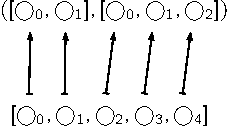
\includegraphics{img/append.pdf}
    \end{center}
    \label{fig:append}
    \caption{Concatenación de containers de listas}
\end{figure}

La reubicación de posiciones se representa en la figura con la flechas. De esta forma, para el caso particular del ejemplo, la función \AgdaFunction{splitFin} reubicará las posiciones de la siguiente manera:  
  \begin{align*}
\AgdaFunction{splitFin}\ 0 &= \AgdaInductiveConstructor{inj$_1$}\ {0}\\
\AgdaFunction{splitFin}\ 1 &= \AgdaInductiveConstructor{inj$_1$}\ {1}\\
\AgdaFunction{splitFin}\ 2 &= \AgdaInductiveConstructor{inj$_2$}\ {0}\\      
\AgdaFunction{splitFin}\ 3 &= \AgdaInductiveConstructor{inj$_2$}\ {1}\\
\AgdaFunction{splitFin}\ 4 &= \AgdaInductiveConstructor{inj$_2$}\ {2}
  \end{align*}
  
  Si extendemos el morfismo \AgdaFunction{append} sobre los naturales, obtendremos una función de pares de listas de naturales en listas de naturales. Podemos aplicar esta función al par de listas del ejemplo \ref{ex:parlistas} y obtener una lista del cero al siete.
  
\ExecuteMetaData[latex/Examples.tex]{l}

Para convertir una lista de tipo \AgdaDatatype{List} en una definida inductivamente para así poder observar y analizar los resultados más simplemente, contamos con la siguiente función:

\ExecuteMetaData[latex/Examples.tex]{tolist}

Al evaluar \AgdaFunction{ListTo[] ceroAsiete} obtenemos efectivamente una lista de naturales del cero al siete:

\AgdaNumber{0} \cons (\AgdaNumber{1} \cons (\AgdaNumber{2} \cons (\AgdaNumber{3} \cons (\AgdaNumber{4} \cons (\AgdaNumber{5} \cons (\AgdaNumber{6} \cons (\AgdaNumber{7} \cons \AgdaInductiveConstructor{[]})))))))

\end{example}

\section{Inicial y terminal}
\subsection{Motivación: (De)construyendo los objetos inicial y terminal}
\label{mot:initterm}
En las diversas secciones de motivación de cada construcción universal teníamos como objetivo el introducir la noción categórica a partir de pensar en teoría de conjuntos, yendo de lo particular a lo general. 

¿Cómo hablar del conjunto vacío sin referirnos a sus elementos, o mejor dicho, a la ausencia de ellos? La estrategia es siempre pensar en los morfismos, o en este caso, en las funciones; podemos entonces reformular la pregunta: ¿Qué relaciones se pueden establecer entre el conjunto vacío y el resto de los conjuntos?, ¿qué funciones podemos construir desde o hacia el conjunto vacío?

Hacia el conjunto vacío resulta imposible construir cualquier función.
Si pensamos por un momento e intentamos construir dicha función, nos resultará imposible, puesto que el conjunto vacío carece de elementos que oficien de recorrido de la función.

Por otro lado, es muy simple construir una función {\it desde} el conjunto vacío hacia cualquier otro objeto, simplemente por el hecho de no necesitar proveer ningún valor. La función vacía será la única función que podamos construir. Hemos encontrado una característica del conjunto vacío: siempre existe una única función desde él hacia cualquier otro conjunto. Es este atributo el que le da el nombre de {\it objeto inicial}
a su generalización en teoría de categorías. En la definición \ref{cat:initial} se expone formalmente.

Como ya hemos comentado en reiteradas ocasiones, si revertimos el sentido de los morfismos en una categoría $\C$ obtenemos una nueva categoría, la categoría dual $\C^{op}$. Allí encontramos los duales de cada construcción, en particular, de la construcción de objeto inicial: el objeto {\it terminal}. Si dijimos que un objeto es inicial cuando siempre exista un morfismo único hacia cualquier otro objeto, uno terminal será aquél con morfismos únicos {\it desde} cualquier otro objeto. En la categoría $\Set$ contamos con muchos objetos terminales. Cualquier conjunto con un único elemento posee la propiedad de aceptar una única función desde cualquier otro conjunto hacia él: la función constante.


\subsection{Definición y formalización}
\begin{definition}\label{cat:initial}

 Un objeto $\bot$ en una categoría $\C$ se dice {\it inicial} si por cada objeto $A$ de $\C$ hay exactamente un morfismo $\flecha{\bot}{}{A}$ desde él.
\begin{center}
  \xymatrixcolsep{3pc}
  \centerline{\xymatrix{ 
      \bot \ar@{-->}[r]^{!}  & A  }}
\end{center}

\end{definition}

\begin{definition}\label{cat:term}

 Un objeto $\top$ en una categoría $\C$ se dice {\it terminal} si por cada objeto $A$ de $\C$ hay exactamente un morfismo $\flecha{A}{}{\top}$ hacia él.
\begin{center}
  \xymatrixcolsep{3pc}
  \centerline{\xymatrix{ 
      A \ar@{-->}[r]^{!} & \top}}
\end{center}

\end{definition}


Damos a continuación la implementación en Agda de estos conceptos. Una categoría $\C$ : \AgdaDatatype{Category} tendrá objeto inicial si podemos proveer una instancia del record definido en el código \ref{code:cat:initial}.  Para ello habrá que individualizar un objeto \AgdaField{Initial}. Además, para poder proclamar la existencia de un morfismo único desde el objeto inicial hacia todo otro objeto, se requiere una forma de construir un habitante de \AgdaField{Hom} $\C$ \AgdaField{Initial} $X$, para todo $X$ y una prueba de su unicidad.

\begin{agdacode}{\it Formalización de categoría con objeto inicial}\hspace{3ex}\label{code:cat:initial}
  
\ExecuteMetaData[latex/Cat.tex]{hasInitial}
\end{agdacode}

Asimismo, proveer una instancia de \AgdaRecord{HasTerminal} $\C$, record definido en el código \ref{code:cat:terminal}, es prueba formal de la existencia de objeto terminal en la categoría $\C$.

\begin{agdacode}{\it Formalización de categoría con objeto terminal}\hspace{3ex}\label{code:cat:terminal}
  
\ExecuteMetaData[latex/Cat.tex]{hasTerminal}
\end{agdacode}

Para ver formalizado lo analizado al comenzar la sección, se expone a continuación los objetos inicial y terminal de la categoría de conjuntos.


\begin{agdacode}{\it Formalización de $\Set$ como categoría con objeto inicial}\hspace{3ex}\label{code:set:initial}
  
\ExecuteMetaData[latex/CatSet.tex]{setHasInitial}
\end{agdacode}

\begin{agdacode}{\it Formalización de $\Set$ como categoría con objeto terminal}\hspace{3ex}\label{code:set:terminal}
  
\ExecuteMetaData[latex/CatSet.tex]{setHasTerminal}
\end{agdacode}

Observemos que para el caso del objeto terminal, expuesto en el código \ref{code:set:terminal}, podríamos haber elegido cualquier conjunto de un elemento. La función \AgdaField{toTermMor} será simplemente la función que retorne el único elemento del conjunto. La garantía de que dicha función es única la provee el campo \AgdaField{isUniqueToTermMor}.


\subsection{Containers vacío y unitario}


%%%%%INICIAL

En esta sección proveeremos instancias de las formulaciones recientemente expuestas, para el caso de la categoría $\Cont$ de containers.

Si pensamos en que tenemos como objetivo proveer un container inicial tal que siempre exista un morfismo único desde él hacia cualquier otro objeto, entonces podemos empezar pensando en los morfismos. Un morfismo de containers se compone, por un lado, de una función entre formas y por otro de una función en posiciones. Quisiéramos que la construcción a proveer posea inherentemente una única función en formas y, elegida una forma, una única en posiciones. De lo analizado en la sección \ref{mot:initterm} de motivación, podemos intuir que el conjunto de las formas deberá ser el vacío. Llamamos \AgdaFunction{Zero} al container inicial:

\ExecuteMetaData[latex/Empty.tex]{Zero}

Como hemos expresado, el morfismo único constará de dos funciones únicas, las funciones vacías. Lo llamamos \AgdaFunction{Zero$_{m}$}.

\ExecuteMetaData[latex/Empty.tex]{Zerom}

Proveemos también la demostración de la unicidad del morfismo \AgdaFunction{Zero$_{m}$}, apelando al lema \AgdaFunction{mEq} y a los postulados de extensionalidad, utilizados de forma trivial con las funciones vacías. 

\ExecuteMetaData[latex/Empty.tex]{ZeromUnique}


En el código \ref{hasInitial} se presenta la instancia completa, garantizando que la categoría $\Cont$ cuenta con objeto inicial. 

\begin{agdacode}{\it Formalización de $\Cont$ como categoría con objeto inicial} \label{hasInitial}

  \ExecuteMetaData[latex/CatCont.tex]{hasInitial}
\end{agdacode}


Notar que así como hemos pensado en construir el objeto inicial de la categoría de containers a partir de la definición e intuición expresadas previamente, podríamos también haberlo motivado como la introducción de aquél container que representa al tipo vacío. Pensado de esa forma, observemos que ya contamos con una forma de construirlo, puesto que el container vacío no es más que el container constante presentado en el ejemplo \ref{cont:k}, instanciado en el conjunto vacío:

\sangrar
\AgdaFunction{Zero} $=$ \AgdaFunction{cK} $\bot$

%%%%%TERMINAL

De la misma forma, el container unitario es aquél que construye el tipo que alberga a un único elemento. Podemos pensarlo como un container constante instanciado en el tipo $\top$ con un único elemento, \AgdaInductiveConstructor{tt}.

\sangrar
\AgdaFunction{One} $=$ \AgdaFunction{cK} $\top$

Sin embargo, es posible demostrar que cualquier conjunto con un único elemento funciona igual de bien, con lo que podemos concluir que el objeto terminal no es único en la categoría de containers, como no lo era en $\Set$.
En teoría de categorías, las restricciones sobre los objetos siempre se dan a través de restricciones sobre los morfismos.
Esto es así porque el nivel de abstracción no nos permite analizar cada objeto en particular más que a partir de observar su relación con otros objetos. Esta es la razón por la que no hablaremos de igualdad entre los objetos. Serán los isomorfismos, i.e. ciertos morfismos particulares, los que otorgarán una forma de referirnos a objetos que comparten propiedades equivalentes.   
Es posible demostrar que el objeto terminal, tanto como el inicial, siempre que existan serán únicos salvo isomorfismos únicos.

Retomando la exposición en la categoría de containers, si desplegamos la definición de \AgdaFunction{cK}, vemos que \AgdaFunction{One} es el container con forma única, sin posiciones.

\ExecuteMetaData[latex/Unit.tex]{One}


El morfismo único hacia el container terminal resulta del morfismo único hacia el conjunto unitario por el lado de las formas y la función vacía por el lado de las posiciones.

\ExecuteMetaData[latex/Unit.tex]{Onem}

A continuación, la prueba de la unicidad de esta construcción. 

\ExecuteMetaData[latex/Unit.tex]{OnemUnique}


Finalmente, en el código \ref{hasTerminal} proveemos una instancia de \AgdaFunction{HasTerminal} $\Cont$:

\begin{agdacode}{\it Formalización de $\Cont$ como categoría con objeto inicial} \label{hasTerminal}

\ExecuteMetaData[latex/CatCont.tex]{hasTerminal}
\end{agdacode}

\section{Exponencial}\label{cons:exp}

\subsection{Motivación: (De)construyendo el exponencial}

Nos interesa comenzar esta sección evocando una problemática simple de la combinatoria de la matemática discreta y preguntarnos: ¿cuántas funciones existen entre dos conjuntos cualesquiera $A$ y $B$?

En la figura \ref{fig:funciones} vemos un ejemplo muy sencillo de dos conjuntos $A$ y $B$ y tres funciones posibles de un conjunto al otro. Se muestran las posibilidades dada una elección determinada de asignación al elemento $a_1$. Tenemos tantas opciones de mapeo para $a_2$ como elementos hay en $B$. La misma cantidad de alternativas existen para asignar a $a_1$.


\begin{figure}[H] 
\begin{center}
  \xymatrixcolsep{0.5pc} \xymatrixrowsep{2pc}
  \centerline{
  \xymatrix{ 
      A \ = & \{ a_{1}, \ar@{|->}[d]  & a_{2} \ar@{|->}[dl]   \} \\
      B \ = & \{ b_{1}, & b_{2}, & b_{3} \} }
  \quad
  \xymatrix{ 
       \{ a_{1},  \ar@{|->}[d] & a_{2}, \ar@{|->}[d] \} \\
       \{ b_{1}, & b_{2} , & b_{3}\} }
    \quad
  \xymatrix{ 
       \{ a_{1},  \ar@{|->}[d] & a_{2}, \ar@{|->}[dr]  \} \\
       \{ b_{1}, & b_{2}, & b_{3} \} }}
  %% \vspace{2ex}
  %% \centerline{
  %% \xymatrix{ 
  %%     \hspace{4ex}& \{ a_{1}, \ar[dr]  & a_{2} \ar[dl]   \} \\
  %%     \hspace{4ex}& \{ b_{1}, & b_{2}, & b_{3} \} }
  %% \quad
  %% \xymatrix{ 
  %%      \{ a_{1},  \ar[dr] & a_{2}, \ar[d] \} \\
  %%      \{ b_{1}, & b_{2} , & b_{3}\} }
  %%   \quad
  %% \xymatrix{ 
  %%      \{ a_{1},  \ar[dr] & a_{2}, \ar[dr]  \} \\
  %%      \{ b_{1}, & b_{2}, & b_{3} \} }}
  %% \vspace{2ex}
  %% \centerline{
  %% \xymatrix{ 
  %%     \hspace{4ex}& \{ a_{1}, \ar[drr]  & a_{2} \ar[dl]   \} \\
  %%     \hspace{4ex}& \{ b_{1}, & b_{2}, & b_{3} \} }
  %% \quad
  %% \xymatrix{ 
  %%      \{ a_{1},  \ar[drr] & a_{2}, \ar[d] \} \\
  %%      \{ b_{1}, & b_{2} , & b_{3}\} }
  %%   \quad
  %% \xymatrix{ 
  %%      \{ a_{1},  \ar[drr] & a_{2}, \ar[dr]  \} \\
  %%      \{ b_{1}, & b_{2}, & b_{3} \} }}
\label{fig:funciones}
\end{center}
\caption{Algunas funciones entre los conjuntos $A$ y $B$ }
\end{figure}

Observemos que si los conjuntos $A$ y $B$ tienen respectivamente $a$ y $b$ cantidad de elementos, tenemos, por cada elemento de $A$, $b$ opciones de mapeos; entonces existen $$\underbrace{b \times b \times  \cdots  b}_{a \text{ veces}} = b^{a}$$
funciones posibles. Por dicha razón, al conjunto de las funciones de $A$ hacia $B$ le asignamos el nombre de exponencial de $B$ a la $A$, y lo simbolizamos $B^{A}$.

En resumen, en la categoría $\Set$ de conjuntos y funciones, el objeto exponencial entre dos objetos $A$ y $B$ que denominamos $B^{A}$, es el conjunto de las funciones de $A$ en $B$. 

Para empezar a pensar en las funciones hacia cada conjunto exponencial, consideremos las funciones $f(\_,\_) : A \times B \to C$.
Al fijar un elemento $a \in A$ obtenemos una nueva función $f(a,\_) : B \to C$; en otras palabras, $f(a,\_) \in C^{B}$. Si hacemos nuevamente variar $a$ entre los elementos de $A$, obtenemos una nueva función que llamamos $\floor{f}$ tal que $$\floor{f} : A \to C^{B}$$ $$\floor{f} (a) = f(a, \_)$$
La función $\floor{f}$ suele llamarse {\it currificación} de $f$ en honor al matemático Haskell B. Curry. Definimos la currificación de una función $f$ como $\floor{f} (a)(b) = f(a,b)$. 

En resumidas cuentas, cualquier función que reciba dos argumentos puede ser currificada y obtener así una nueva función que recibe un solo argumento, retornando una función. Sin embargo, seguir el camino inverso también es posible; para toda función $g : A \to C^{B}$ existe una única $\ceil{g} : A \times B \to C$ tal que $g = \floor{\ceil{g}}$. Podemos definirla como: $$\ceil{g}(a,b) = g(a)(b)$$  

Es simple de probar que nos encontramos --para cada conjunto $C^B$-- frente a una serie de isomorfismos en $\Set$, uno por cada conjunto $A$. Si tenemos las funciones $f : A \times B\to C$ y $g : A\to C^{B}$ entonces vemos que se cumple que las dos posibles composiciones de las funciones $\floor{\_}$ y $\ceil{\_}$ dan como resultado las respectivas identidades.

$\ceil{\floor{f}}(a,b) = \floor{f}(a)(b) = f(a,b) $

$\floor{\ceil{g}}(a)(b) = \ceil{g}(a,b) = g(a)(b) $

\subsection{Definición y formalización}
Antes de continuar con la presentación categórica del objeto exponencial, veamos otro ejemplo de funtor que puede encontrarse en las categorías que cuentan con productos, y que nos será necesario para continuar con la exposición.

\begin{definition}\label{homprod}
Sea $\C$ una categoría con productos. Dados dos objetos $B$ y $C$ de $\C$, el funtor $Hom_{\C}(\_\times B, C)$ desde la categoría $\C^{op}$ hacia la categoría $\Set$ mapea:

  \begin{itemize}
  \item cada objeto $A$ de $\C$ hacia el conjunto de morfismos $Hom_{\C}(A\times B, C)$
  \item cada morfismo $\flecha{A'}{f}{A}$ hacia la función de post-composición $$\_ \circ (f \times \id{B}) : Hom_{\C}(A\times B,C) \to Hom_{\C}(A'\times B,C)$$
  \end{itemize}
  El siguiente diagrama muestra cómo transformamos un morfismo del primer conjunto en uno del segundo a partir de la post-composición, vemos cómo en la categoría $\C$, de componer un morfismo $\flecha{A\times B}{h}{C}$ con el morfismo $\flecha{A'\times B}{f \times \id{B}}{A\times B}$ obtenemos un morfismo de $A'\times B$ hacia $C$. 

\begin{center}
  \xymatrixcolsep{4pc} \xymatrixrowsep{4pc}
  \centerline{\xymatrix{
          A \times B \ar[r]^{h} & C  \\
      A ' \times B \ar[u]^{f \times \id{B}} \ar[ur]_{h \circ (f \times \id{B})} & } \qquad
}
\end{center}
  
\end{definition}

En el código asociado a la tesina se puede encontrar la formalización y prueba de este funtor,  
%% A continuación, la formalización y parte de la prueba de que dicha construcción es en efecto un funtor,
que habremos de llamar \AgdaFunction{HomProd}.
%% \begin{agdacode}{\it Formalización del funtor Hom$_{\C}(\_\times Y , Z)$} \label{code:homProd}
    
%% \ExecuteMetaData[latex/HomFunctor.tex]{homProd}  
%% \end{agdacode}

\begin{definition}\label{cat:exp}
  Sea $\C$ una categoría que cuenta con productos y sean $B$ y $C$ dos de sus objetos. Un objeto $C^{B}$ es el {\it exponencial} de $C$ a la $B$ siempre que exista un isomorfismo natural entre los funtores {\it Hom}$(\_\times B, C)$ y {\it Hom}$(\_, C^{B})$.

  Al igual que con el coproducto y el producto, diremos que una categoría {\it cuenta con exponenciales} cuando para todo par de objetos existe el exponencial entre ellos.
\end{definition}

Del análisis de la definición observamos que para que un objeto $C^B$ sea exponencial deberá existir una transformación natural $\floor{\_}: \mathit{Hom}(\_\times B, C) \Rightarrow \mathit{Hom}(\_,C^B)$ tal que para cada $A$, cada una de sus componentes $\floor{\_}_{A}$ es un isomorfismo. Llamaremos $\ceil{\_}_{A}$ a cada una de las inversas. El siguiente diagrama lo expresa de una forma alternativa. La doble línea indica la presencia de un isomorfismo.

\begin{center}
\xymatrixcolsep{1pc}
  \begin{minipage}{0.1\linewidth}
    \begin{center}
      \centerline{ \xymatrix{ {} \\ {}  \ar@/^/^{\ceil{\_}_{A}}[u] }}
    \end{center}
  \end{minipage}
  \begin{minipage}{0.2\linewidth}
    \vspace{2ex}
    \begin{center}
      \centerline{ \infer={A \to C^B}{A\times B\to C} }
    \end{center}
  \end{minipage}
  \begin{minipage}{0.1\linewidth}
    \begin{center}
      \centerline{ \xymatrix{ {} \ar@/^/^{\floor{\_}_{A}}[d] \\ {} }}
    \end{center}
  \end{minipage}
\end{center}

Para apreciar mejor las consecuencias de la ley de naturalidad que obtenemos de la transformación natural $\floor{\_}$, observemos el siguiente diagrama conmutativo. Para todo par de objetos $A$ y $A'$ y morfismo $f : A' \to A$ de la categoría $\C^{op}$, el siguiente diagrama deberá conmutar.

\begin{center}
  \xymatrixcolsep{4pc} \xymatrixrowsep{3pc}
  \centerline{\xymatrix{ 
      \mathit{Hom}(A\times B,C) \ar[r]^{\_\circ(f\times \id{B})} \ar@/_/[d]_{\floor{\_}_{A}} & \mathit{Hom}(A'\times B,C) \ar@/_/[d]_{\floor{\_}_{A'}}\\
      \mathit{Hom}(A,C^B) \ar[r]_{\_ \,\circ\, f} \ar@/_/[u]_{\ceil{\_}_{A}}& \mathit{Hom}(A',C^B)  \ar@/_/[u]_{\ceil{\_}_{A'}}
}}
\end{center}
Además de los isomorfismos ya mencionados, se deberá pedir que se cumpla la ley de naturalidad dada por: $$\floor{g \circ (f \times \id{B})}_{A'} \cong \floor{g}_{A} \circ f \qquad \mbox{ para todo } g : A\times B \to C$$

Finalmente formalizamos el hecho de que una categoría $\C$ cuente con exponenciales con la estructura presentada en el código \ref{code:hasExponentials}. El campo \AgdaField{Exp} construye el objeto exponencial a partir de otros dos cualesquiera. El elemento \AgdaField{floor} es la transformación natural entre los funtores mencionados anteriormente, siendo el campo \AgdaField{nat} la formalización de la ley de naturalidad. Finalmente, el campo \AgdaField{ceil} construye cada uno de los isomorfismos requeridos, y la garantía de serlo está dada por los elementos \AgdaField{iso$_1$} e \AgdaField{iso$_2$}. 

\begin{agdacode}{\it Formalización de categoría con exponenciales}\label{code:hasExponentials}
 
\ExecuteMetaData[latex/Cat.tex]{hasExponentials}
\end{agdacode}

\begin{remark} Teniendo formalizados el concepto de isomorfismo natural (código \ref{code:natiso}) y los funtores \AgdaFunction{Hom$_1$} y \AgdaFunction{HomProd} (código \ref{code:hom1} y definición \ref{homprod}), podríamos haber formalizado \AgdaRecord{HasExponentials} como un record que contuviera simplemente al constructor \AgdaField{Exp} y un isomorfismo natural entre los funtores mencionados. Para mayor claridad, evitamos en este caso la construcción de records anidados.   
\end{remark}

\subsection{Exponencial de Containers}
En esta sección veremos que la categoría $\Cont$ de containers cuenta con exponenciales~\cite{alti:2010} y expondremos su formalización.

Con el objetivo presentar el exponencial de containers de la forma más comprensible posible, lo introduciremos a partir del análisis de un ejemplo, para luego presentarlo de forma general.

\begin{example} {\it Currificando} \AgdaFunction{append} 

  Para comenzar, recordemos que tenemos como objetivo construir, dados dos containers $B$ y $C$, su container exponencial, al que llamaremos $C$ \AgdaFunction{$\hat{\ }$} $B$. Dicho container deberá satisfacer las reglas de la definición, esto es, deberá existir un isomorfismo natural entre los siguientes morfismos de containers:

  $$
 \infer={A\ \AgdaFunction{$\Rightarrow$}\ C\ \AgdaFunction{$\hat{\ }$}\ B}{\AgdaDatatype{Both}\ A\ B\ \AgdaFunction{$\Rightarrow$}\ C} 
$$

 El morfismo \AgdaFunction{append} es un caso particular de morfismo de la parte superior del isomorfismo, instanciando $A$, $B$ y $C$ con el container \AgdaFunction{cList}.

   \ExecuteMetaData[latex/Examples.tex]{appendt}

   Buscamos construir un morfismo \AgdaFunction{curryappend} de tipo \AgdaDatatype{cList $\Rightarrow$ cList $\hat{\ }$ cList} isomorfo a \AgdaFunction{append}, es decir, sin pérdida de información, manteniendo la posibilidad de reconstruir \AgdaFunction{append} a partir de \AgdaFunction{curryappend}. Para ello, recordemos (ver ejemplo \ref{example:append}, pág. \pageref{example:append}) que el morfismo de concatenación arma un container de lista de longitud igual a la suma de las longitudes de las listas argumento; por otro lado, reubica las posiciones según la función \AgdaFunction{splitFin}, como se puede apreciar en la figura \ref{fig:append2}, donde la reubicación se indica con flechas.

\begin{figure}[H]
\begin{minipage}{0.3\textwidth}
\begin{center}
  \xymatrixrowsep{4pc} 
  \centerline{\xymatrix{ 
      \hspace{1ex}\ar@{=>}@/_1pc/[d]_{\mbox{\AgdaFunction{append}}} \\
      \hspace{1ex}
}}
\end{center}
\end{minipage}
     \begin{minipage}{0.7\textwidth}
  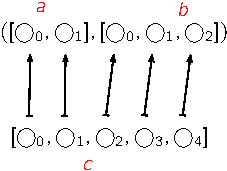
\includegraphics{img/append1.pdf}
     \end{minipage}
     \caption{Concatenación de containers de listas}
     \label{fig:append2}
\end{figure}

Podemos apreciar en la figura \ref{fig:curryappend} un panorama de general de comportamiento de la función \AgdaFunction{curryappend} y un esquema del objeto exponencial. Para referirnos con más exactitud a cada una de los containers de lista, los llamaremos \rojo{$a$}, \rojo{$b$} y \rojo{$c$}, de longitudes 2, 3 y 5 respectivamente. Así como en la figura \ref{fig:append2} representábamos al container producto $(\rojo{a},\rojo{b})$ entre paréntesis, ahora representamos al exponencial dentro del óvalo de la figura \ref{fig:curryappend}.

Las formas posibles del exponencial de dos listas incluirán no sólo una forma de construir la longitud de \rojo{$c$} a partir de las longitudes de las listas \rojo{$a$} y \rojo{$b$}, sino también la información de la reubicación de las posiciones de \rojo{$b$} en las posiciones de \rojo{$c$}. Más aún, se marcarán con un elemento distinguible \AgdaInductiveConstructor{tt} de tipo \AgdaDatatype{$\top$} a aquellas posiciones que se solían asignar a posiciones en \rojo{$a$}. Esto se ve representado en la figura \ref{fig:curryappend} con flechas rectas.

De esta forma, de las únicas posiciones que queda por determinar la procedencia son de aquellas marcadas con el valor \AgdaInductiveConstructor{tt}. Esas posiciones conformarán entonces el conjunto de posiciones del container exponencial. En el ejemplo de la figura \ref{fig:curryappend} encontramos dos de estas posiciones, representadas como aquellas de donde parten las flechas curvas.

\begin{figure}[H] 
\begin{minipage}{0.3\textwidth}
\begin{center}
  \xymatrixrowsep{5pc} 
  \centerline{\xymatrix{ 
      \hspace{1ex}\ar@{=>}@/_1pc/[d]_{\mbox{\AgdaFunction{curryappend}}} \\
      \hspace{1ex}
}}
\end{center}
\vspace{13ex}
\end{minipage}
\begin{minipage}{0.7\textwidth}
  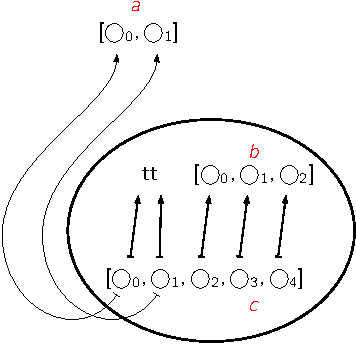
\includegraphics{img/curryappend1.pdf}
\end{minipage}
\caption{Currificación de la función de concatenación}
\label{fig:curryappend}
\end{figure}

Continuaremos con la presentación de este morfismo una vez presentada la construcción del exponencial de containers.
\end{example}


\begin{definition}\label{def:cont:exp}
Definimos al constructor de cada objeto exponencial, el elemento \AgdaFunction{$\_\hat{\ \ }\_$}, como una función que toma dos containers $C$ y $B$ y retorna otro container. 

\ExecuteMetaData[latex/Exponential.tex]{exp}
\end{definition}

Recapitulando, una forma de un container exponencial es, por un lado, una función desde las formas de $B$ hacia las formas de $C$. Además, determinada una forma de $C$, una función que reubique posiciones, mapeando hacia un elemento distintivo \AgdaInductiveConstructor{tt} las posiciones que solían mapearse hacia $A$. Por otra parte, habrá tantas posiciones en un container exponencial como elementos marcados con el valor  \AgdaInductiveConstructor{tt}.

\addtocounter{definition}{-2}
\begin{example}[Continuación] \label{ex:curryappend}

  Para retomar con el ejemplo introductorio, veamos cómo se implementa la función \AgdaFunction{curryappend} ahora que contamos con la definición del exponencial de containers. 

  \ExecuteMetaData[latex/Examples.tex]{curryappend}

  Por un lado, la función de mapeo de formas, de tipo $\AgdaField{Sh}\ \AgdaFunction{cList}  \to (\AgdaField{Sh}\ \AgdaFunction{cList}\ \AgdaFunction{$\hat{}$}\ \AgdaFunction{cList})$, asigna a cada forma $n_1$ de la primera lista una forma del exponencial de las otras dos listas. Esta forma asignada no es ni más ni menos que la función suma, igual que para el caso de \AgdaFunction{append}. Además, incluye una función de posiciones, la misma función \AgdaFunction{splitFin} utilizada en \AgdaFunction{append}, sólo que con los elementos izquierdos del coproducto {\it borrados}, i.e. reemplazados por el elemento \AgdaInductiveConstructor{tt}.
 
La función \AgdaFunction{eraseLeft} transforma un elemento de tipo $A$ \AgdaFunction{$\uplus$} $B$ en uno de tipo \AgdaFunction{$\top$} \AgdaFunction{$\uplus$} $B$, convirtiendo todo elemento de la forma \AgdaInductiveConstructor{inj$_1$}$\, a$ en \AgdaInductiveConstructor{inj$_1$ tt}, dejando igual al resto.

\ExecuteMetaData[latex/Exponential.tex]{eraseLeft}

En cuanto al mapeo de posiciones, obtenemos una posición del primer container a partir de una posición del exponencial haciendo uso de la función \AgdaFunction{fromInj$_1$}, a la que se la provee de una posición $q$ y una prueba de que $q$ era de la forma \AgdaInductiveConstructor{inj$_1$ tt}.

La función \AgdaFunction{fromInj$_1$} toma un valor de tipo $A$ \AgdaFunction{$\uplus$} $B$ y extrae el valor de tipo $A$, provista prueba de que realmente nos encontramos en dicho caso. Cuando no sea así, será absurda la existencia de un habitante de la prueba.  

\ExecuteMetaData[latex/Exponential.tex]{fromInj1}

\end{example}
\addtocounter{definition}{1}

De observar las funciones \AgdaFunction{curryappend} y \AgdaFunction{append}, presentadas en los ejemplos  \ref{ex:curryappend} y \ref{example:append} podemos vislumbrar la forma de construir una función \AgdaFunction{$\curry{\_}$}, que crea un morfismo de tipo $A \ \AgdaFunction{$\Rightarrow$}\  C\ \AgdaFunction{$\hat{\ \ }$}\ B$ a partir de un morfismo $f : \AgdaDatatype{Both}\ A\ B \ \AgdaFunction{$\Rightarrow$}\  C$. El siguiente código muestra su implementación, que hace uso de las funciones auxiliares \AgdaFunction{eraseLeft} y  \AgdaFunction{fromInj$_1$}.

\ExecuteMetaData[latex/Exponential.tex]{floor}


La inversa de la función \AgdaFunction{$\curry{\_}$} es una función \AgdaFunction{$\uncurry{\_}$} dada por:

\ExecuteMetaData[latex/Exponential.tex]{ceil}

donde la función \AgdaFunction{insLeft} se comporta de forma contraria a \AgdaFunction{eraseLeft}, convirtiendo todo elemento de la forma \AgdaInductiveConstructor{inj$_1$ tt} en \AgdaInductiveConstructor{inj$_1$} $x$, y dejando sin modificar los elementos de la forma \AgdaInductiveConstructor{inj$_2$} $y$.

\ExecuteMetaData[latex/Exponential.tex]{insLeft}

Los elementos restantes que componen el record \AgdaRecord{ContHasExponentials} son las pruebas de la naturalidad e isomorfismos. Antes veremos algunas pruebas auxiliares.
La siguiente función prueba que insertar la componente izquierda de un valor, dentro del mismo valor luego de haber borrado a la izquierda, es igual a la identidad:

\ExecuteMetaData[latex/Exponential.tex]{aux1}
La función \AgdaFunction{lema$_2$} afirma que borrar a izquierda luego de insertar a izquierda es lo mismo que no hacer nada:

\ExecuteMetaData[latex/Exponential.tex]{aux2}
Extraer el valor izquierdo luego de haberlo insertado retorna como resultado el mismo valor: 

\ExecuteMetaData[latex/Exponential.tex]{aux3}

Hasta ahora hemos expuesto funciones auxiliares que usarán en las demostraciones de los respectivos isomorfismos, hecho que resulta evidente al observar que en todos los casos probamos que la composición de dos funciones nos da como resultado la identidad. A continuación probaremos dos lemas necesarios para la prueba de la naturalidad. Esta situación también puede vislumbrarse si se observa con atención. 

Borrar a izquierda un coproducto al que se le modificó su componente izquierda es equivalente a borrar el coproducto original:

\ExecuteMetaData[latex/Exponential.tex]{aux4}
Similarmente, extraer de la izquierda luego de haber modificado dicha componente de un coproducto es lo mismo que extraer y luego aplicar la función.

\ExecuteMetaData[latex/Exponential.tex]{aux5}
En los casos donde tengamos que probar la equivalencia de funciones que toman como argumento pares dependientes, será más cómodo probar la equivalencia de las versiones currificadas de dichas funciones. Para ello, utilizamos el siguiente lema.

\ExecuteMetaData[latex/Exponential.tex]{uncurryEq}

Finalmente, las pruebas del isomorfismo y la naturalidad se exponen en los códigos \ref{code:iso1}, \ref{code:iso2} y \ref{code:natural}. Se utilizan los lemas \AgdaFunction{dcong} (código \ref{code:dcong}, pág \pageref{code:dcong}), \AgdaFunction{dext} (código \ref{code:dext}, pág. \pageref{code:dext}) y \AgdaFunction{dSumEq} (código \ref{code:dSumEq}, pág. \pageref{code:dSumEq})

\begin{agdacode}{\it Prueba de un lado del isomorfismo entre \AgdaFunction{$\curry{\_}$} y \AgdaFunction{$\uncurry{\_}$} } \label{code:iso1}

\ExecuteMetaData[latex/Exponential.tex]{iso1}
\end{agdacode}

\begin{agdacode}{\it Prueba del otro lado del isomorfismo entre \AgdaFunction{$\curry{\_}$} y \AgdaFunction{$\uncurry{\_}$}} \label{code:iso2}

  \ExecuteMetaData[latex/Exponential.tex]{iso2}
\end{agdacode}
  
\begin{agdacode}{\it Prueba de la naturalidad de \AgdaFunction{$\curry{\_}$}}\label{code:natural}
      
\ExecuteMetaData[latex/Exponential.tex]{natural}
\end{agdacode}

Presentadas ya cada una de las funciones necesarias para la construcción de una instancia de \AgdaRecord{HasExponential} para el caso de la categoría de containers, el siguiente código las reúne, quedando formalmente demostrado que la categoría $\Cont$ cuenta con exponenciales.

\begin{agdacode}{\it Formalización de $\Cont$ como categoría con exponenciales}\label{code:setHasExponentials}

\ExecuteMetaData[latex/CatCont.tex]{hasExponentials}
\end{agdacode}


\subsection{Categorías Cartesianas Cerradas}\label{cons:ccc}

Un resultado interesante de haber formalizado estas construcciones es el haber demostrado que la categoría $\Cont$ pertenece a un subconjunto de categorías denominadas {\it cartesianas cerradas}.

\begin{definition}
Una categoría $\C$ se denomina {\it cartesiana cerrada} si cuenta con objeto terminal, productos y exponenciales.
\end{definition}

La formalización de dicho concepto en Agda se presenta en el código \ref{code:IsCartesianClosed} y la instancia para la categoría $\Cont$, en el código \ref{code:ContIsCartesianClosed}.
\begin{agdacode}{\it Formalización de categoría cartesiana cerrada}\label{code:IsCartesianClosed}
  
\ExecuteMetaData[latex/Cat.tex]{IsCartesianClosed}
\end{agdacode}
\begin{agdacode}{\it Formalización de $\Cont$ como categoría cartesiana cerrada}\label{code:ContIsCartesianClosed}
  
\ExecuteMetaData[latex/CatCont.tex]{ContIsCartesianClosed}
\end{agdacode}

Como hemos mencionado brevemente en la introducción, la principal relevancia de las categorías cartesianas cerradas se resumen en el hecho de poder ponerlas en correspondencia con el lambda cálculo con tipos simples y la lógica proposicional intuicionista.


\bookmarksetup{startatroot}

\chapter*{Conclusiones}
\addcontentsline{toc}{chapter}{Conclusiones}

La programación genérica tiene como objetivo primordial el reuso de código. Para lograrlo, apela a la construcción de programas cuyos argumentos puedan pertenecer no solo a un tipo de datos particular, sino a un conjunto más amplio.   
Una de las problemáticas principales a la que la programación genérica debe enfrentarse es la de poder definir adecuadamente su ámbito de abstracción. Es decir, para cumplir la meta de construir programas cuyo alcance sea mayor a un único tipo de dato y, en su lugar, funcione para un subconjunto de todos los tipos posibles, es imperativo poder definir con precisión este subconjunto e incluso poder inspeccionar cada habitante de forma individual.

En los lenguajes de tipos dependientes podemos obtener ese subconjunto de forma precisa a partir de definir universos. Estos consisten simplemente en códigos sintácticos, uno por cada tipo a incluir, equipados con una función de extensión que dado un código asigna el tipo de datos que éste representa.

En este trabajo se ha analizado un universo de constructores de tipos en particular, el universo de containers. Se comenzó con un análisis más bien intuitivo, introduciendo múltiples ejemplos. Se expuso la forma de reinterpretar cada container --a partir del cálculo de su extensión-- como un constructor de tipos funtorial, es decir, como un endofuntor en $\Set$. Vistos como universo, los containers resultan ser, entonces, un tipo de códigos sintácticos, siendo su extensión la función de interpretación de dichos códigos hacia los constructores de tipos que representan.  

Se ha mostrado la forma en que los morfismos de containers se erigen como un universo para representar a las funciones paramétricas entre los tipos de datos generados por containers. Estos resultan ser ni más ni menos que las transformaciones naturales entre los mencionados endofuntores que los containers representan. Se probó que es posible componerlos y siempre existe el morfismo identidad.

Debido a la fuerte relación existente entre la teoría de tipos, la lógica y la programación, dar un salto de abstracción y tomar un punto de vista más general, dejando de lado los detalles de la construcción, otorga sin lugar a dudas una garantía de legitimidad siempre apreciada. Este salto se realiza en el momento en que pasamos a analizar las construcciones en el marco de la teoría de categorías.

La generalización es la esencia de las matemáticas. Muchas veces existen similitudes entre objetos de estudio a priori muy distantes, donde las analogías no se encuentran a simple vista. Abstraer, exponer las definiciones en términos categóricos puede implicar también que demostrar teoremas o encontrar propiedades sobre el objeto de estudio resulte más sencillo. En efecto, de no haber sido tomado este punto de vista categórico, no se hubiera llegado al resultado de que los containers cuentan con exponenciales y son aptos para modelar sistemas de alto orden. 

Consecuentemente, se ha expuesto al universo de containers como una categoría denominada $\Cont$, cuyos objetos son containers y sus morfismos, los morfismos de containers. Además, se ha provisto una formalización completa en Agda de esta construcción.

Como punto central del trabajo, se han presentado pruebas formales de que la categoría $\Cont$ cuenta con coproductos, productos, exponenciales, objetos inicial y terminal. 
Particularmente, es una categoría cartesiana cerrada, hecho que la pone en correspondencia con sistemas como el lambda cálculo simplemente tipado o la lógica proposicional intuicionista.

Como se ha expuesto en las preliminares, gracias al isomorfismo de Curry-Howard y al requerimiento de que los programas sean totales, programar en Agda y demostrar teoremas son dos tareas en consonancia. Por lo tanto, haber provisto las pruebas formales de que cada uno de los objetos (producto, coproducto, etc) realmente lo son, según parámetros categóricos, implica haber extendido las librerías de containers existentes al día de hoy.


\subsection*{Trabajos futuros}

En esta tesina se ha presentado el universo de containers {\it de único argumento}. Es decir que se ha trabajado a partir de una definición de container donde, al momento de calcular su extensión, se obtienen endofuntores en $\Set$ de solamente un argumento. Un evidente posible camino a seguir es extender la formalización para incluir containers a más de un argumento.  

Una vez realizado este avance, será posible también formalizar el hecho de que la categoría de containers es cerrada bajo álgebras iniciales y coálgebras finales.

Otras extensiones que son posibles de realizarse a partir de las contribuciones de este trabajo son las referidas a la función de extensión, que lleva a cualquier habitante del universo de containers hacia un endofuntor en la categoría de conjuntos. Es posible generalizar dicha función para que resulte en un endofuntor en cualquier categoría extensa y localmente cartesiana cerrada. Además, propiedades como que dicho funtor es totalmente fiel pueden ser formalizadas y así garantizar que los morfismos de containers resulten ser, en efecto, todas y solo todas las transformaciones naturales entre los definidos endofuntores. 

En lo que se refiere al uso de las contribuciones realizadas, se espera que la biblioteca provista sirva como universo para programar genéricamente sobre un subconjunto acotado de tipos de datos, provistas las garantías de que dicho universo es cerrado bajo una serie interesante de construcciones. Por otro lado, se espera que sea un buen aporte como punto de partida para futuras formalizaciones. 









\begin{appendices}
\chapter{Hoja de ruta del código fuente}\label{guia}

La contribución principal del presente trabajo es una librería de containers extendida con las formalizaciones de la clausura de la categoría con respecto al producto, coproducto, exponencial y la existencia de objetos terminal e inicial. Actualmente está alojada en un repositorio {\it Git} situado en el siguiente enlace: \gitcode. Allí se puede encontrar todo el código Agda analizado en este trabajo, así como también porciones de código menos relevantes que no fueron expuestas, e incluso este documento. A continuación se expondrá un pantallazo general del contenido del mencionado repositorio. Para visualizar más claramente su estructura, observar la figura \ref{fig:map} (pág. \pageref{fig:map}).

En la carpeta \texttt{doc} se puede encontrar el texto completo de esta tesina, cuyo archivo \LaTeX\ principal es \texttt{main.tex}, compilable realizando \texttt{make}. En la subcarpeta \texttt{simplecode} se encuentra el código, simplificado para su exposición y anotado para la compilación del documento.

El resto de los archivos corresponden a la formalización en sí. Los archivos relacionados a la formalización de la teoría de categorías se encuentran en el archivo \texttt{Category.agda} y en la carpeta \texttt{Category}. El archivo \texttt{Extras.agda} contiene definiciones auxiliares utilizadas en muchas de las demostraciones. La formalización de containers se encuentra distribuida en los archivos almacenados en la carpeta \texttt{Container} y los archivos \texttt{Container.agda}.  
Cada una de las construcciones sobre containers se encuentra en un archivo distinto.

\begin{figure}[h]
\dirtree{%
.1 /.
  .2 \textcolor{blue}{doc}.
    .3 main.tex.
    .3 \textcolor{blue}{simplecode}.
  .2 Extras.agda.
  .2 Category.agda.
  .2 \textcolor{blue}{Category}.
    .3 Coproduct.agda.
    .3 \textcolor{blue}{Examples}.
      .4 Fun.agda.
      .4 Sets.agda.
    .3 Exponential.agda.
    .3 Funtor.agda.
    .3 HomFunctors.agda.
    .3 Initial.agda.
    .3 Isomorphism.agda.
    .3 Natural.agda.
    .3 Product.agda.
    .3 Representables.agda.
    .3 Terminal.agda.
  .2 Container.agda.
  .2 \textcolor{blue}{Container}.
    .3 Composition.agda.
    .3 Coproduct.agda.
    .3 Examples.agda.
    .3 Exponential.agda.
    .3 Initial.agda.
    .3 Product.agda.
    .3 Terminal.agda.
}
\caption{Organización de los directorios del proyecto}\label{fig:map}
\end{figure}

\end{appendices}

\backmatter

\chapter{Bibliograf\'{i}a}

\bibliographystyleIntro{babalpha}
\bibliographyIntro{bib/bibintro}
\addcontentsline{toc}{section}{Referencias históricas}

\newcommand{\nombredelabiblio}{Bibliograf\'{i}a general}
\renewcommand\bibname{\nombredelabiblio}

\bibliographystyle{babalpha}
\bibliography{bib/biblio}
\addcontentsline{toc}{section}{\nombredelabiblio}


\end{document}




